\documentclass[a4paper,11pt]{book}
\usepackage[utf8]{inputenc}
\usepackage[T1]{fontenc}
\usepackage[danish]{babel}
\usepackage{graphicx}
\usepackage{amsmath}
\usepackage{listings}
\usepackage{xcolor}
\usepackage[hidelinks]{hyperref}
\usepackage{fancyhdr}
\usepackage{titlesec}

% Definer farver
\definecolor{codegreen}{rgb}{0,0.6,0}
\definecolor{codegray}{rgb}{0.5,0.5,0.5}
\definecolor{codepurple}{rgb}{0.58,0,0.82}
\definecolor{backcolour}{rgb}{0.95,0.95,0.92}

% Kode listning stil
\lstdefinestyle{mystyle}{
	backgroundcolor=\color{backcolour},   
	commentstyle=\color{codegreen},
	keywordstyle=\color{magenta},
	numberstyle=\tiny\color{codegray},
	stringstyle=\color{codepurple},
	basicstyle=\ttfamily\footnotesize,
	breakatwhitespace=false,         
	breaklines=true,                 
	captionpos=b,                    
	keepspaces=true,                 
	numbers=left,                    
	numbersep=5pt,                  
	showspaces=false,                
	showstringspaces=false,
	showtabs=false,                  
	tabsize=2
}

\lstset{style=mystyle}

% Forbedret titelside format
\title{\Huge\textbf{Industriel Netværksteknologi:}\\[0.5cm]\Huge\textbf{Fra Teori til Praksis}}
\author{\vspace{2cm}\LARGE Anders S. Østergaard}
\date{\vfill\today}

% Fjern header og tilpas footer
\pagestyle{plain} % Standard sidetal i footeren, men ingen header

% Undertrykke sidetal på forsiden, indholdsfortegnelse, partsider og blanke sider
\usepackage{fancyhdr}
\fancypagestyle{plain}{
	\fancyhf{} % Fjern header og footer
	\renewcommand{\headrulewidth}{0pt} % Fjern header-linjen
	\renewcommand{\footrulewidth}{0pt} % Fjern footer-linjen
	\fancyfoot[C]{\thepage} % Tilføj sidetal i footeren (kun sidetal)
}

% Fjern sidetal på forsiden, indholdsfortegnelse og blanke sider
\let\cleardoublepage\clearpage
\makeatletter
\renewcommand{\maketitle}{%
	\begin{titlepage}
		\centering
		\vspace*{5cm}
		{\Huge\bfseries \@title \par}
		\vspace{2cm}
		{\Large \@author \par}
		\vfill
		{\large \@date \par}
	\end{titlepage}
	\thispagestyle{empty} % Ingen sidetal på forsiden
}
\renewcommand{\tableofcontents}{\@starttoc{toc}\thispagestyle{empty}} % Ingen sidetal på indholdsfortegnelsen
\makeatother

% Undertrykke sidetal på \part sider
\titleformat{\part}[display]
{\normalfont\huge\bfseries\centering} % Format for part
{\partname\ \thepart}                  % Label
{20pt}                                 % Spacing
{\Huge}                                % Before-code
\titlespacing*{\part}{0pt}{0pt}{40pt}

\begin{document}
	
	\maketitle
	\clearpage
	\tableofcontents
	\thispagestyle{empty}
	\newpage
	
	% Introduktion
	\part{Intro}
\chapter{Introduktion}
\label{chapter:introduktion}
Dette dokument er en samlet ressource til dokumentation af de netværksopgaver, der er udført med henblik på konfiguration og styring af automatiseringssystemer ved hjælp af TIA Portal, Studio 5000, Universal Robots og ABB's robotteknologi. Målet med dokumentet er at skabe en overskuelig guide, som kan assistere teknikere, studerende og undervisere indenfor automatiseringsteknologi med at forstå og udføre netværksrelaterede opgaver på tværs af forskellige automatiseringssystemer.
\newline\newline
\noindent Rapporten er opdelt i to hoveddele: Ethernet-baserede netværk og bus-baserede netværk. I TIA Portal-sektionen vil vi gennemgå opsætningen af kommunikationsnetværk for Siemens automatiseringshardware, hvilket inkluderer konfiguration af PROFINET. I Studio 5000-afsnittet vil fokus være på integrationen af Allen-Bradley udstyr og hvordan man opsætter Ethernet/IP netværk til industriel automatisering. For Universal Robots vil dokumentationen dække opsætningen af netværksforbindelser til UR-robotter, herunder fjernstyring og scriptkommunikation. Endelig vil ABB-robotafsnittet give vejledning i konfiguration af netværksparametre for ABB's robotter, med særlig opmærksomhed på RobotStudio.
\newline\newline
\noindent Hver sektion vil indeholde skridt-for-skridt vejledning, eksempler på konfigurationsfiler og fejlfindingstips for at sikre, at læseren kan navigere i opgaverne med tillid. Dokumentet er tænkt som en levende ressource, der kan opdateres og udvides, efterhånden som teknologierne udvikler sig og flere erfaringer bliver indarbejdet.

\section{Historie}
\label{section:historie}
For at forstå den nuværende tilstand og fremtidige retning for industrielle netværk, er det nyttigt at se på deres historiske udvikling. Her er nogle nøglepunkter i denne udvikling:

\subsection{Tidlige Systemer}
Før udbredelsen af digitale netværk blev industrielle systemer typisk styret af enkeltstående kontrolenheder og analog kommunikation. Dette resulterede i begrænset funktionalitet og fleksibilitet.

\subsection{Fremkomsten af PLC'er}
Programmable Logic Controllers (PLC'er) blev introduceret i 1960'erne og 1970'erne som en måde at automatisere og styre industrielle processer mere effektivt. PLC'er banede vejen for mere komplekse og fleksible automatiseringsløsninger.

\subsection{Serielle Protokoller}
I 1980'erne begyndte brugen af serielle kommunikationsprotokoller som RS232, RS422 og RS485 at blive almindelig i industrielle netværk, hvilket muliggør mere pålidelig dataoverførsel mellem enheder.
\newline\newline\noindent\textbf{RS232, RS422, RS485:} Disse er blandt de tidligste standarder for seriel kommunikation, introduceret i henholdsvis 1960'erne og 1970'erne. RS232 var en af de første bredt anvendte kommunikationsstandarder, der tillod forbindelse mellem computere og modemmer. RS422 og RS485 blev udviklet som forbedringer til RS232, hvor de tilbyder længere kabellængder og understøtter flere enheder på samme netværk. Disse standarder blev grundlaget for mange tidlige automatiseringssystemer.

\subsection{Fieldbus Teknologier}
I 1990'erne blev Fieldbus-protokoller som Profibus og DeviceNet udviklet, hvilket gjorde det muligt at forbinde mange enheder på et enkelt netværk med mere komplekse kommunikationsbehov.
\newline\newline\noindent\textbf{PROFIBUS (Process Field Bus):} Introduceret i 1980'erne, er PROFIBUS en af de tidligste standarder for feltbus kommunikation i industriel automatisering. Den blev udviklet for at standardisere kommunikationen mellem kontrolsystemer og feltudstyr, som f.eks. sensorer og aktuatorer. PROFIBUS understøtter både diskret og procesautomatisering og har været en af de mest udbredte industrielle netværksstandarder.
\newline\newline\noindent\textbf{DeviceNet:} DeviceNet, udviklet i 1990'erne, er baseret på CAN (Controller Area Network) og tilbyder en netværksløsning, der især fokuserer på lav-niveau enhedsforbindelser, såsom sensorer og aktuatorer. Den understreger enkelthed og omkostningseffektivitet i automatiseringssystemer.
\newline\newline\noindent\textbf{AS-I Bus (Actuator Sensor Interface):} AS-I Bus, introduceret i begyndelsen af 1990'erne, er designet som en simpel og omkostningseffektiv løsning til forbindelse af binære sensorer og aktuatorer. Det giver en nem måde at implementere en sensor/aktuator-niveau netværksinfrastruktur.

\section{Ethernet-baserede Netværk}
I slutningen af 1990'erne og begyndelsen af 2000'erne blev Ethernet-baserede netværk som Ethernet/IP og Profinet introduceret. Disse teknologier udnyttede de høje hastigheder og standardiserede kommunikationsprotokoller fra IT-verdenen og tilpassede dem til industrielle behov.
\newline\newline\noindent
\textbf{PROFINET:} Som opfølgeren til PROFIBUS, introduceret i begyndelsen af 2000'erne, er PROFINET en industriel Ethernet-standard designet til at imødekomme behovet for højere datahastigheder og realtid kommunikation. PROFINET udnytter standard Ethernet-teknologi og er optimeret til industrielle applikationer, hvilket giver større fleksibilitet og ydeevne.
\newline\newline\noindent
\textbf{Ethernet/IP:} Ethernet/IP, indført i slutningen af 1990'erne, er en industriel netværksstandard, der kombinerer traditionel Ethernet-teknologi med industriel protokol (CIP - Common Industrial Protocol). Den tilbyder en omfattende kommunikationsløsning, der understøtter både diskret og procesautomatisering.
\newline\newline\noindent
\textbf{Modbus RTU og TCP:} Modbus, udviklet i slutningen af 1970'erne af Modicon (nu Schneider Electric), er en af de ældste og mest udbredte kommunikationsprotokoller i industrien. Modbus RTU (Remote Terminal Unit) er en seriel kommunikationsprotokol, der anvender RS485 standarden, mens Modbus TCP/IP er en version af Modbus, der bruger Ethernet til kommunikation, hvilket gør det muligt at anvende standard netværksinfrastruktur til industriel kommunikation.
\begin{figure}[!h]
	\centering
	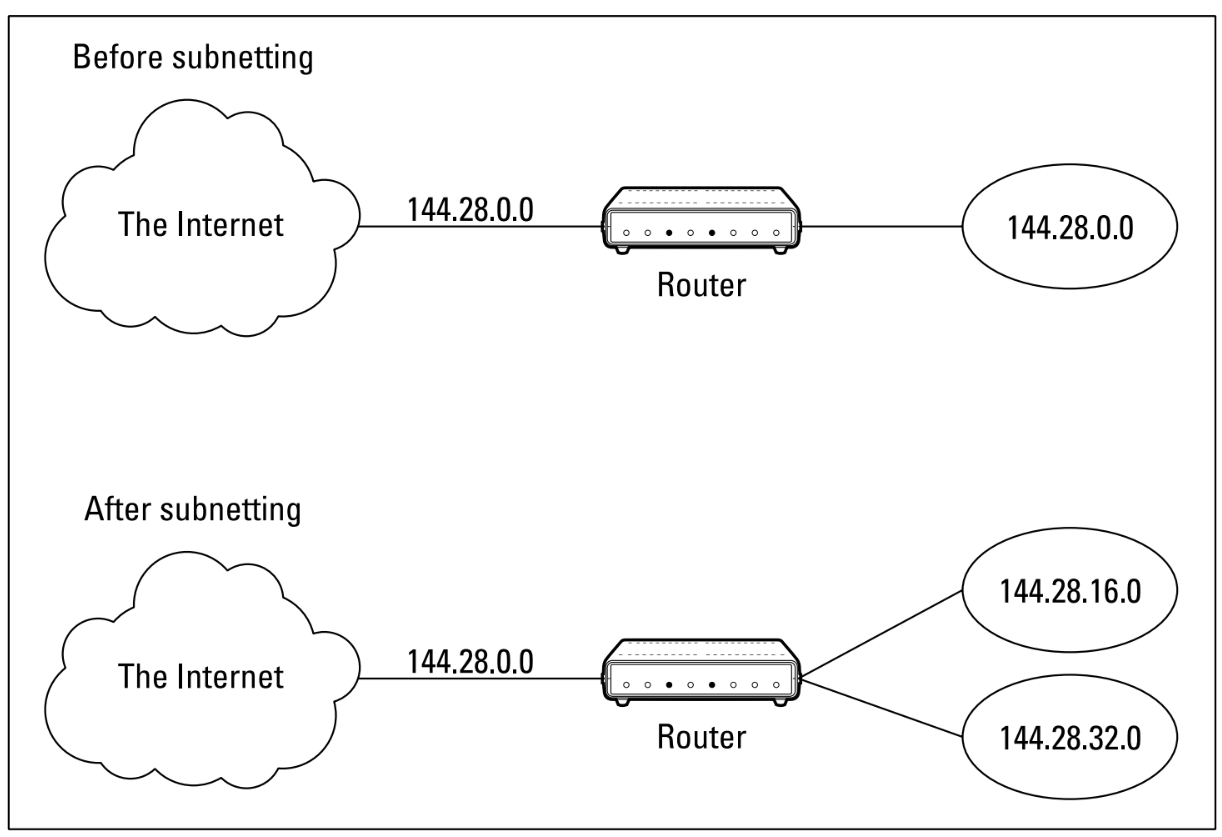
\includegraphics[width=\textwidth]{fig/fig32}
	\caption{Historisk visning af protokoller og standarder}
\end{figure}

\section{Industri 4.0 og IoT}
I det sidste årti har fremkomsten af Industri 4.0 og Internet of Things (IoT) revolutioneret industrielle netværk ved at integrere avancerede sensorer, cloud computing og big data-analyse, hvilket fører til mere intelligente og forbundne produktionssystemer.
\newline\newline\noindent
\textbf{IO-Link:} IO-Link, som blev standardiseret i 2006, er en punkt-til-punkt kommunikationsteknologi, der anvendes til at forbinde intelligente sensorer og aktuatorer til et automatiseringssystem. IO-Link er designet til at overføre både procesdata og diagnostiske data og giver mulighed for detaljeret sensor- og aktuatorstyring.
\clearpage
	% Fundamentale IT-Netværksteknologier
	\part{Fundamentale IT-Netværksteknologier}
\chapter{Introduktion til IT-Netværk}
\label{chapter:Grundlæggende_Netværksteori}
\section{Grundlæggende Netværksbegreber}
Netværk er systemer, der forbinder computere og andre enheder for at dele ressourcer og information. Der findes flere typer netværk, hver med specifikke egenskaber og anvendelser.

\section{Hvad er et netværk?}
Et netværk består af flere enheder (f.eks. computere, printere, servere) forbundet sammen for at dele data og ressourcer. Netværk muliggør kommunikation, samarbejde og adgang til information på tværs af geografiske afstande. De anvender forskellige teknologier og protokoller for at sikre effektiv og sikker dataoverførsel.

\section{Netværkstyper}
\begin{itemize}
	\item \textbf{LAN (Local Area Network):} Et LAN er et lokalt netværk, der dækker et lille geografisk område som et kontor, en skole eller en bygning. Det giver højhastighedsforbindelse mellem enheder inden for et begrænset område og bruges til at dele ressourcer som printere og filer.
	\item \textbf{WAN (Wide Area Network):} Et WAN dækker et større geografisk område, som en by, et land eller endda flere lande. Internettet er det mest kendte eksempel på et WAN. WAN'er forbinder flere LAN'er og andre netværk for at muliggøre kommunikation og dataudveksling over lange afstande.
	\item \textbf{MAN (Metropolitan Area Network):} Et MAN dækker et byområde eller en stor campus og forbinder flere LAN'er inden for denne region. Det giver højhastighedsforbindelser og bruges ofte af store organisationer eller kommunale myndigheder.
\end{itemize}

\section{Netværkets betydning}
Netværk spiller en afgørende rolle i den moderne verden ved at muliggøre:
\begin{itemize}
	\item \textbf{Deling af ressourcer:} Netværk tillader flere enheder at dele hardware (f.eks. printere) og software (f.eks. applikationer), hvilket reducerer omkostninger og øger effektiviteten.
	\item \textbf{Kommunikation:} Netværk muliggør hurtig og pålidelig kommunikation gennem e-mails, chat, videokonferencer og andre kommunikationsværktøjer.
	\item \textbf{Dataadgang:} Brugere kan få adgang til og dele data og filer på tværs af enheder og geografiske placeringer, hvilket fremmer samarbejde og informationsdeling.
	\item \textbf{Sikkerhed og administration:} Netværk gør det muligt at centralisere sikkerhed og administration, hvilket gør det lettere at implementere og håndhæve sikkerhedspolitikker og administrere ressourcer.
\end{itemize}

\section{Netværkshardware}
For at opbygge og vedligeholde netværk er det nødvendigt at bruge specifikke hardwarekomponenter. Her er en forklaring af de mest essentielle netværkshardwareenheder.

\subsection{Repeaters og Hubs}
En \textbf{repeater} er en enhed på lag 1 i OSI-modellen, designet til at omgå den maksimale længdebegrænsning af twisted-pair netværkskabler. En repeater har to RJ45-porte, som er internt forbundet via en forstærker. Elektriske signaler, der modtages på en af portene, forstærkes og sendes gennem den anden port. Dermed kan kabler på begge sider af repeateren være op til 100 meter lange, hvilket effektivt fordobler rækkevidden af kablet.
\newline
\newline
\noindent En \textbf{hub} er en repeater med flere porte. For eksempel kan en hub have fire eller otte porte. Disse porte kan forbinde til andre enheder på netværket såsom en klientcomputer, en server eller en printer. En port på en hub kan også forbindes til en anden hub, hvilket gør det muligt at forbinde flere enheder sammen. For eksempel kan en otte-ports hub forbinde syv computere og en anden otte-ports hub, hvilket kan forbinde til yderligere syv computere. På denne måde kan to otte-ports hubs forbinde 14 computere til hinanden.
\newline
\newline
\noindent Der er to vigtige ting at vide om hubs:
\newline
\newline
\noindent Den første og vigtigste ting at vide om hubs er, at de næsten aldrig bruges længere. Det skyldes, at switches, som opererer på lag 2 i OSI-modellen, er mere effektive og almindeligt anvendt i moderne netværk.
\newline
\newline
\noindent Den anden vigtige ting at vide om hubs er, at et elektrisk signal modtaget på en af hubbens porte forstærkes og gentages på alle de andre porte i hubben. Således vil en enhed tilsluttet en af portene kunne se signalerne fra alle andre enheder tilsluttet de andre porte. For eksempel, i en otte-ports hub, vil et signal modtaget på port 1 blive forstærket og sendt ud til portene 2 til 8. På samme måde vil signaler modtaget på port 4 blive forstærket og sendt ud til portene 1 til 3 samt 5 til 8.

\begin{figure}[h!]
	\centering
	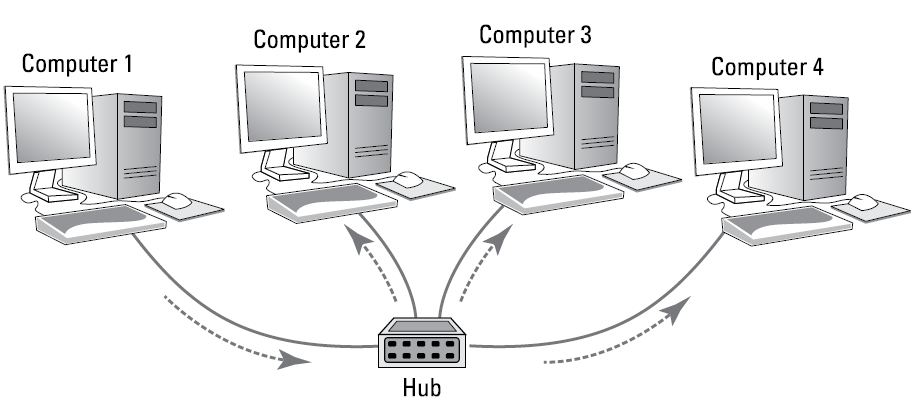
\includegraphics[width=0.7\textwidth]{fig/fig39}
	\caption{Diagram over en repeater og hub forbindelser}
	\label{fig:repeater_hub}
\end{figure}
\noindent En hub er en simpel netværksenhed, der forbinder flere enheder i et LAN (Local Area Network). Den sender data, den modtager, til alle de enheder, der er forbundet til den, uden at tage hensyn til hvilken enhed dataene er beregnet til. Dette medfører ineffektiv dataoverførsel, da unødvendige data sendes til alle tilsluttede enheder. Hubs opererer på det fysiske lag (Layer 1) i OSI-modellen og har begrænset effektivitet sammenlignet med switches, som kun sender data til den specifikke modtager enhed.

\subsection{Switches}
En \textbf{switch} er en mere avanceret netværksenhed, der opererer på lag 2 i OSI-modellen (datalinklaget). I modsætning til hubs, der sender data til alle tilsluttede enheder, sender en switch data kun til den specifikke enhed, som dataene er beregnet til. Dette gøres ved at opretholde en MAC-adressetabel, som kortlægger hver port til en specifik MAC-adresse.
\newline
\newline
\noindent Switches har flere fordele sammenlignet med hubs:
\begin{itemize}
	\item \textbf{Effektivitet:} Fordi switches kun sender data til den specifikke modtager, reduceres unødvendig netværkstrafik, hvilket forbedrer den samlede netværkseffektivitet.
	\item \textbf{Sikkerhed:} Data sendes kun til den tilsigtede modtager, hvilket reducerer risikoen for, at data fanges op af andre enheder på netværket.
	\item \textbf{Ydeevne:} Switches kan håndtere flere samtidige forbindelser uden at forårsage kollisioner, hvilket er et almindeligt problem med hubs.
\end{itemize}
\begin{figure}[!h]
	\centering
	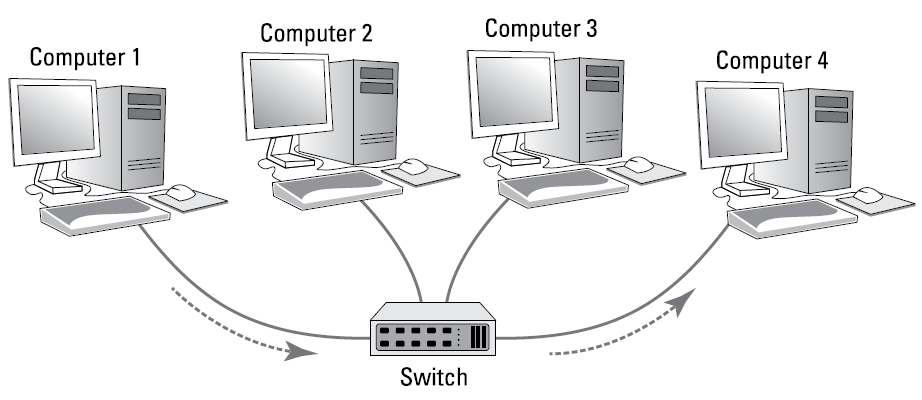
\includegraphics[width=.7\textwidth]{fig/fig40}
	\caption{Switch}
\end{figure}

\subsection{Routere}
En \textbf{router} er en lag 3-enhed, hvilket betyder, at den arbejder på netværkslaget i OSI-modellen. I praksis betyder det, at routere arbejder med IP-adresser. Routere er afgørende for at forbinde forskellige netværk og styre netværkstrafikken mellem dem. En router adskiller sig fra en switch på flere måder:
\begin{itemize}
	\item \textbf{IP-adresser:} Switches arbejder med MAC-adresser og ved ingenting om IP-adresser. I kontrast arbejder routere med IP-adresser.
	\item \textbf{Kommunikation mellem subnetværk:} Routere kan facilitere kommunikation mellem IP-netværk med forskellige subnet. For eksempel, hvis din organisation har et 10.0.100.x netværk og et 192.168.0.x netværk, kan en router muliggøre, at pakker kan rejse fra 10.0.100.x netværket til 192.168.0.x netværket og omvendt.
	\item \textbf{Internetforbindelse:} Routere muliggør også, at et privat netværk kan kommunikere med internettet. For eksempel, hvis du vil forbinde dit netværk til internettet via en bredbåndsudbyder, skal du bruge en router til at udveksle pakker mellem dit private netværk og internettet via den offentlige IP-adresse.
\end{itemize}

\begin{figure}[h!]
	\centering
	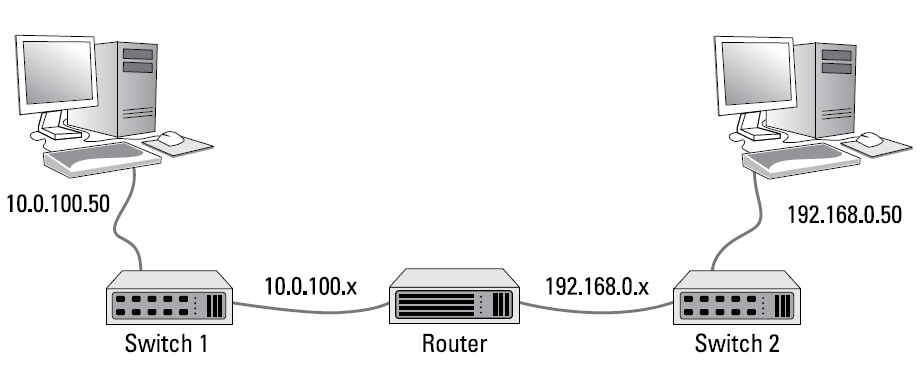
\includegraphics[width=0.8\textwidth]{fig/fig41}
	\caption{To IP-netværk forbundet via en router}
	\label{fig:router}
\end{figure}
\noindent Den grundlæggende funktion af en router er ganske simpel. Overvej det simple netværk afbilledet i figur \ref{fig:router}. Her har en organisation to separate IP-netværk, et med 10.0.100.x subnet og et andet med 192.168.0.x subnet. En router bruges til at forbinde disse to netværk. På begge sider af routeren er der en switch, og hver switch har kun en computer forbundet.
\newline
\newline
\noindent Routeren bruger IP-adresser til at bestemme den bedste vej for data at rejse fra kilden til destinationen. Når en computer på det ene netværk ønsker at sende data til en computer på det andet netværk, sender den først dataene til switchen. Switch 1 videresender dataene til routeren, som derefter bestemmer den bedste vej og sender dataene videre til Switch 2, som til sidst sender dataene til den rigtige destination.

\subsection{Modems}
Et modem (modulator-demodulator) er en enhed, der konverterer digitale data fra en computer til analoge signaler, der kan overføres over telefonlinjer eller kabelnetværk og omvendt. Modemer bruges til at forbinde computere til internettet, især på steder hvor der ikke er tilgængelige bredbåndsforbindelser.

\section{Sammenhæng mellem Netværkshardware}
For at opbygge et effektivt og pålideligt netværk er det vigtigt at forstå, hvordan disse hardwarekomponenter arbejder sammen:
\begin{itemize}
	\item \textbf{Interaktion mellem routere og switches:} Routere forbinder forskellige netværk, mens switches forbinder enheder inden for samme netværk. I et typisk netværk vil en switch forbinde computere og andre enheder i et LAN, og en router vil forbinde dette LAN til internettet.
	\item \textbf{Brug af hubs i små netværk:} Hubs kan anvendes i små netværk med få enheder, hvor effektiviteten ikke er et stort problem. I større netværk vil switches være mere effektive på grund af deres evne til at videresende data specifikt til den tiltænkte modtager.
	\item \textbf{Modemer til internetadgang:} Modemer bruges til at oprette forbindelse til internettet ved at konvertere digitale signaler til analoge og omvendt. De kan arbejde sammen med routere for at distribuere internetadgang til flere enheder i et netværk.
\end{itemize}

\section{Circuit Switching og Packet Switching}
I netværkskommunikation findes der to grundlæggende metoder til dataoverførsel: circuit switching og packet switching. 

\subsection{Circuit Switching}
Circuit switching indebærer oprettelsen af en dedikeret kommunikationskanal mellem to enheder for hele varigheden af en kommunikationssession. Dette er ligesom det traditionelle telefonsystem, hvor en linje er reserveret til en samtale fra start til slut. Fordelen ved circuit switching er, at det sikrer en kontinuerlig og stabil forbindelse, hvilket er ideelt til overførsel af data, der kræver konstant båndbredde. Ulempen er, at denne metode kan være ineffektiv og dyr, da ressourcerne forbliver allokeret, selv når der ikke sendes data.

\subsection{Packet Switching}
Packet switching, derimod, bryder dataene op i mindre pakker, som sendes individuelt gennem netværket. Hver pakke kan tage forskellige ruter til sin destination, afhængigt af netværksforholdene. Ved ankomsten samles pakkerne i den korrekte rækkefølge af modtagerens system. Denne metode er mere effektiv, da netværksressourcerne deles mellem flere brugere, hvilket muliggør optimal udnyttelse af båndbredden. Packet switching anvendes i de fleste moderne datanetværk, såsom internettet, hvor det sikrer fleksibel og pålidelig dataoverførsel.

\subsection{Forbindelsesorienteret og Forbindelsesløs Kommunikation}
Packet-switched netværk kan tilbyde både forbindelsesorienterede og forbindelsesløse kommunikationer. Forbindelsesorienteret kommunikation, som f.eks. TCP (Transmission Control Protocol), etablerer en virtuel forbindelse, hvor dataoverførslerne er struktureret og pålidelige. Forbindelsesløs kommunikation, som f.eks. UDP (User Datagram Protocol), sender data uden at etablere en vedvarende forbindelse, hvilket er hurtigere men mindre pålideligt.

\subsection{Praktisk Anvendelse}
I moderne industrielle netværk anvendes packet switching bredt på grund af dets evne til at håndtere store datamængder effektivt. Denne teknologi gør det muligt at sende data fra mange forskellige kilder samtidigt, hvilket er afgørende for komplekse automationssystemer, hvor forskellige sensorer og enheder konstant kommunikerer.
\newline
\newline
\noindent Sammenfattende er forståelsen af både circuit switching og packet switching vigtig for at kunne designe og implementere effektive netværksløsninger, der opfylder specifikke behov for stabilitet, hastighed og effektivitet.

\section{Media Access Control (MAC) mechanisms}
Medieadgangskontrolmekanismer er essentielle for at regulere, hvordan data sendes og modtages i netværk. Der er tre primære metoder, der anvendes til at styre adgangen til mediet: Master-slave, Token-passing og CSMA/CD.

\subsection{Master-slave (eller forespørgsel-svar) metode}
Master-slave metoden, også kendt som forespørgsel-svar metoden, anvendes ofte i netværk, hvor en central node (master) skal kommunikere med flere underordnede noder (slaver). I denne opsætning styrer masternoden kommunikationen ved at sende forespørgsler til slavenoderne og vente på svar. Processen fungerer således:
\begin{itemize}
	\item Masternoden sender en besked til den første slave i rækken, der enten anmoder om data eller sender data til slaven.
	\item Alle slavenoder modtager beskeden, men kun den node, hvis adresse matcher beskedens destination, reagerer. De andre noder ignorerer beskeden.
	\item Den adresserede slavenode læser beskeden og kontrollerer for eventuelle fejl. Hvis der opdages fejl, såsom uoverensstemmelser i checksummen, afvises beskeden.
	\item Hvis en slave ikke reagerer, forsøger masternoden at kontakte den op til tre gange, før den går videre til den næste slave i rækken.
	\item Denne cyklus fortsætter, indtil alle slavenoder er blevet kontaktet, hvilket udgør en fuld forespørgselscyklus.
\end{itemize}
Fordelen ved denne metode er enkelheden i opsætningen og den fulde kontrol, masternoden har over kommunikationen. Dette gør det nemt at administrere dataflowet, især når hver slave har en forudsigelig mængde data. Ulempen er dog, at systemet kan være ineffektivt, hvis en slave har behov for at sende uforudsete mængder data, eller hvis der opstår behov for hurtig overførsel af kritiske data.

\subsection{Token-passing}
Token-passing er en metode, hvor kontrollen over netværket overføres mellem noder via en særlig besked kaldet en token. Denne metode bruges ofte i netværk, der kræver pålidelig og garanteret dataoverførsel, såsom industrielle kontrolsystemer. Token-passing fungerer på følgende måde:
\begin{itemize}
	\item En node modtager token-beskeden fra en nærliggende node og får dermed kontrol over netværket.
	\item Noden beholder token i en bestemt tidsperiode eller indtil den har sendt sine beskeder.
	\item Noden sender derefter data til andre noder og overfører token til den næste node i rækken.
	\item Denne proces gentages, hvilket sikrer, at alle noder får en chance for at sende data inden for et givet tidsrum.
\end{itemize}
Fordelen ved token-passing er, at det sikrer deterministisk adgang til mediet, hvilket betyder, at alle noder får lige mulighed for at sende data. Dette er især vigtigt i systemer, hvor tidssensitive dataoverførsler er afgørende. Eksempler på netværk, der anvender token-passing, inkluderer Arcnet (stjernetopologi), Modbus (bustopologi) og IBM token ring (ringtopologi).

\subsection{CSMA/CD (Carrier Sense Multiple Access/Collision Detection)}
CSMA/CD er en enkel og effektiv metode til at regulere datatrafik i et netværk. Denne metode anvendes ofte i netværk som Ethernet og fungerer ved, at noder lytter efter ledig båndbredde, før de sender data. CSMA/CD processen er som følger:
\begin{itemize}
	\item En node, der ønsker at sende data, lytter først efter aktivitet på netværket. Hvis netværket er ledigt, begynder noden at sende data.
	\item Under transmissionen sammenligner noden de sendte data med de data, der er til stede på netværket. Hvis der opdages en kollision (dvs. to noder sender samtidig), stopper transmissionen øjeblikkeligt.
	\item De kolliderende noder venter en tilfældig periode, før de forsøger at sende igen, hvilket reducerer risikoen for yderligere kollisioner.
\end{itemize}
CSMA/CD er enkel og effektiv, især i netværk med let trafik. Dog kan metoden blive ineffektiv ved høj trafikbelastning, da kollisioner kan blive hyppige og forsinke dataoverførsler. Det mest almindelige eksempel på CSMA/CD er Ethernet.

\section{Transmissionsteknikker}
Transmissionsteknikker beskriver, hvordan data overføres over et netværk. De to mest anvendte teknikker er baseband og broadband.

\subsection{Baseband}
Baseband transmission er en metode, hvor hele båndbredden af mediet anvendes af en enkelt kommunikationskanal ad gangen. Denne teknik er karakteriseret ved, at signalet sendes direkte uden modulation, hvilket betyder, at den elektriske signalspænding varierer direkte med dataene.
\begin{itemize}
	\item \textbf{Tidssignalering (TDM):} Baseband transmission bruger ofte tidsdeling multiplexing (Time Division Multiplexing, TDM), hvor hver enhed tildeles en bestemt tidslomme til at transmittere data. Dette sikrer, at kun én enhed sender data ad gangen, hvilket eliminerer risikoen for kollisioner.
	\item \textbf{Anvendelse:} Denne metode er almindeligt anvendt i Ethernet-netværk, specielt i det oprindelige 10BASE-T Ethernet, hvor data sendes over twisted pair-kabler uden behov for yderligere modulation.
	\item \textbf{Fordele:}
	\begin{itemize}
		\item Simpel og nem at implementere.
		\item Lav omkostning på grund af enkelheden i udstyr og kabling.
	\end{itemize}
	\item \textbf{Ulemper:}
	\begin{itemize}
		\item Begrænset rækkevidde og båndbredde sammenlignet med broadband.
		\item Ikke velegnet til lange afstande uden brug af repeatere.
	\end{itemize}
\end{itemize}

\subsection{Broadband}
Broadband transmission er en metode, hvor mediets båndbredde opdeles i flere kanaler, som hver især kan transmittere data samtidigt. Dette gøres ved at modulere dataene på forskellige frekvensbærere, hvilket tillader flere signaler at dele samme fysiske medie uden at interferere med hinanden.
\begin{itemize}
	\item \textbf{Frekvensdeling (FDM):} Broadband bruger frekvensdeling multiplexing (Frequency Division Multiplexing, FDM), hvor hver kanal tildeles en specifik frekvensbånd. Dette muliggør parallel transmission af data fra flere enheder.
	\item \textbf{Anvendelse:} Broadband transmission anvendes typisk i kabelnetværk og fiberoptiske netværk, hvor høj båndbredde og lange afstande er nødvendige. Eksempler inkluderer kabel-tv og bredbåndsinternetforbindelser.
	\item \textbf{Fordele:}
	\begin{itemize}
		\item Høj båndbredde, hvilket muliggør hurtigere dataoverførsel.
		\item Kan transmittere over længere afstande uden behov for repeatere.
	\end{itemize}
	\item \textbf{Ulemper:}
	\begin{itemize}
		\item Mere komplekst og dyrere at implementere.
		\item Kræver specialiseret udstyr til modulation og demodulation.
	\end{itemize}
\end{itemize}
Data transmitteres ved at modulere en bærebølge med informationen, hvilket gør det muligt at udnytte større båndbredder og tillade højere dataoverførselshastigheder. Koaksialkabler og optiske fibre er typisk foretrukne medier for FDM på grund af deres høje båndbreddekapacitet.
\newline
\newline
\noindent Disse transmissionsteknikker og medieadgangskontrolmekanismer spiller en afgørende rolle i design og implementering af effektive og pålidelige netværk, både i kommercielle og industrielle applikationer. 
\newline
\newline
\noindent\textbf{Eksempel:} Profinet bruger både Ethernet-standarder (CSMA/CD) og har specifikationer for det fysiske lag, hvilket gør det til en robust løsning for industrielle netværk.

\section{OSI-modellen og dens anvendelse i industrielle netværk}
Open Systems Interconnection (OSI) modellen er en konceptuel ramme, der bruges til at forstå og implementere standarder for netværkskommunikation. Modellen opdeler netværkskommunikation i syv forskellige lag, hvor hvert lag har specifikke funktioner og tjenester. Disse lag er designet til at interagere med hinanden på en standardiseret måde, hvilket muliggør kommunikation mellem forskellige netværksudstyr og protokoller.

\subsection{Lag 1: Fysisk Lag}
Det fysiske lag er det nederste lag i OSI-modellen. Det håndterer den fysiske forbindelse mellem enheder og den faktiske transmission og modtagelse af data i form af elektriske signaler, lys eller radiobølger. Dette lag omfatter hardwarekomponenter som kabler, switches og netværkskort. I industrielle netværk inkluderer dette lag også miljømæssige faktorer som elektromagnetisk interferens og temperaturvariationer, hvilket kan påvirke dataoverførslen.

\subsection{Lag 2: Datalink Lag}
Datalink laget er ansvarligt for pålidelig dataoverførsel mellem to enheder på samme netværk. Det opdeler data i frames og håndterer fejlkorrektion fra det fysiske lag. Datalink laget består af to underlag: Media Access Control (MAC) og Logical Link Control (LLC). I industrielle netværk bruges protokoller som EtherCAT og PROFINET på dette lag for at sikre hurtig og pålidelig dataoverførsel mellem kontroller og feltudstyr.

\subsection{Lag 3: Netværks Lag}
Netværks laget styrer routing af data mellem forskellige netværk. Dette lag opdeler data i pakker og bestemmer den bedste vej til destinationen ved hjælp af routingprotokoller som IP (Internet Protocol). Netværks laget håndterer også logiske adressering. I industrielle netværk bruges ofte avancerede routingteknikker til at sikre, at data når deres destination hurtigt og effektivt, selv i komplekse netværksstrukturer.

\subsection{Lag 4: Transport Lag}
Transport laget er ansvarligt for pålidelig dataoverførsel mellem to endepunkter. Det opdeler data i segmenter og sikrer, at dataene når frem uden fejl og i den rigtige rækkefølge. Protokoller som TCP (Transmission Control Protocol) og UDP (User Datagram Protocol) opererer på dette lag. I industrielle netværk er transportlaget afgørende for at sikre, at kontrolsignaler og dataoverførsler er præcise og pålidelige.

\subsection{Lag 5: Session Lag}
Session laget styrer etablering, vedligeholdelse og afslutning af kommunikationssessioner mellem applikationer. Det sikrer, at sessioner forbliver adskilte og organiserer dataudveksling i sessioner. I industrielle applikationer bruges dette lag til at administrere vedvarende forbindelser mellem kontrolsystemer og deres tilhørende enheder, hvilket sikrer kontinuerlig drift og overvågning.

\subsection{Lag 6: Præsentations Lag}
Præsentations laget er ansvarligt for datatranslation, datakomprimering og datakryptering. Det sørger for, at data, der sendes fra applikationslaget, er i et format, der kan forstås af modtagerens applikationslag. I industrielle netværk kan dette lag være involveret i konvertering af dataformater mellem forskellige systemer og sikring af, at data er korrekt krypteret for sikkerhedsmæssige formål.

\subsection{Lag 7: Applikations Lag}
Applikations laget er det øverste lag i OSI-modellen og fungerer som grænseflade mellem netværkstjenester og applikationssoftware. Det tilbyder tjenester som e-mail, filoverførsel og webbrowseradgang. Protokoller som HTTP, FTP og SMTP opererer på dette lag. I industrielle netværk omfatter dette lag også specialiserede applikationer til processtyring, overvågning og dataindsamling, hvilket gør det muligt for operatører at interagere med og styre industrielle systemer.
\begin{figure}[!h]
	\centering
	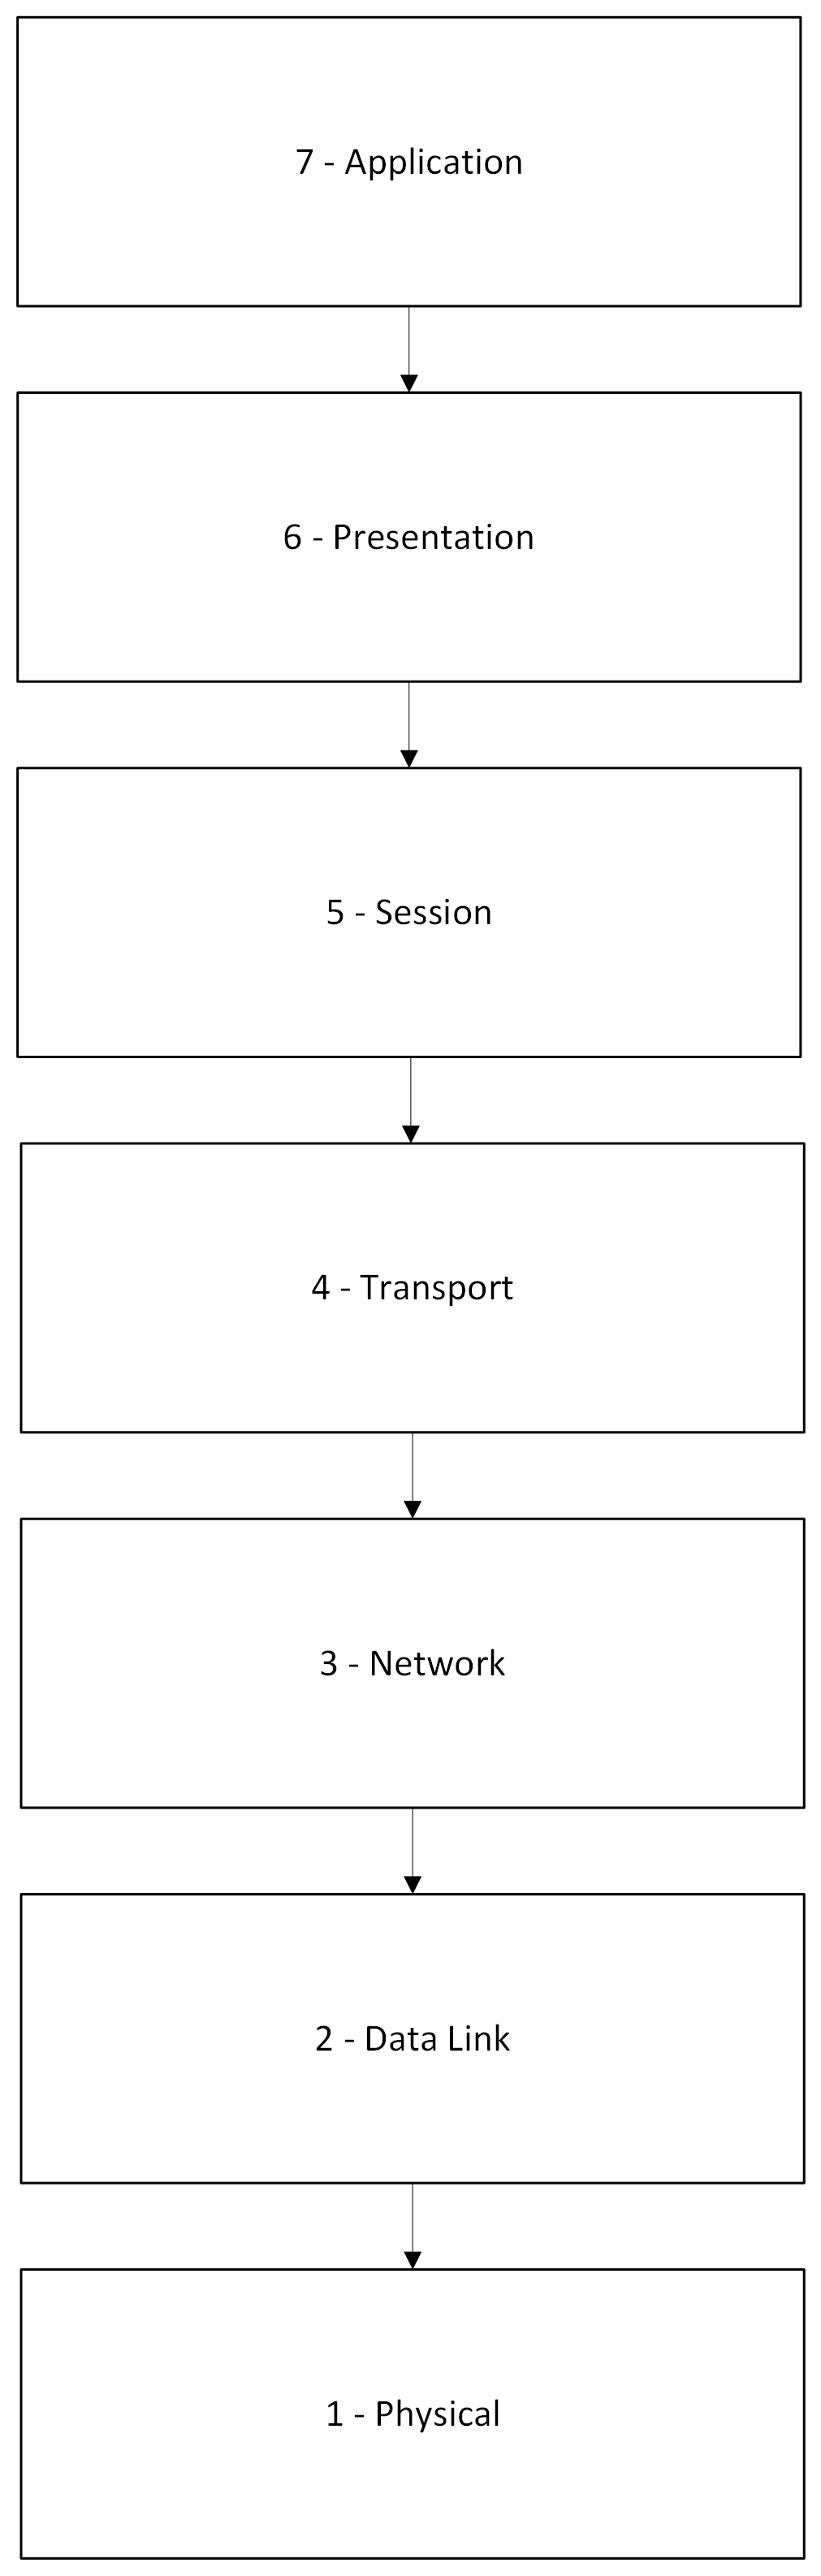
\includegraphics[width=0.3\textwidth]{fig/fig1.png} % Inkluder billedet af OSI-modellen her
	\caption{Illustration af OSI-modellens syv lag}
	\label{fig:osi_model}
\end{figure}

\subsection{Sammenhæng mellem lagene}
Hvert lag i OSI-modellen kommunikerer direkte med de lag, der er umiddelbart over og under det. Data, der sendes fra en applikation, bevæger sig ned gennem lagene, hvor hver lag tilføjer sine egne specifikke oplysninger (f.eks. headers og trailers), inden de transmitteres over netværket. Ved modtagelse bevæger dataene sig op gennem lagene, hvor hver lag fjerner sine tilsvarende oplysninger og videresender de relevante data til det næste lag.
\begin{itemize}
	\item \textbf{Fordele ved OSI-modellen:}
	\begin{itemize}
		\item Standardisering: Tilbyder en standardiseret ramme for netværkskommunikation.
		\item Interoperabilitet: Muliggør interoperabilitet mellem forskellige netværksprodukter og -teknologier.
		\item Modularitet: Tillader udvikling og fejlfinding af individuelle lag uden at påvirke de andre lag.
	\end{itemize}
\end{itemize}
For en visuel forståelse, se Figur \ref{fig:osi_model}, som illustrerer OSI-modellens syv lag og deres funktioner.

\subsection{Anvendelse af OSI-modellen i industrielle netværk}
I industrielle netværk anvendes OSI-modellen til at designe og implementere netværksinfrastrukturer, der opfylder specifikke krav til pålidelighed, sikkerhed og effektivitet. Hvert lag i OSI-modellen bidrager til den samlede funktionalitet og ydeevne af netværket.
\newline
\newline
\noindent\textbf{Eksempel på Anvendelse: PROFINET}
PROFINET er en industriel Ethernet-standard, der bruger OSI-modellen som grundlag. PROFINET opererer primært på datalinklaget (Lag 2) og netværkslaget (Lag 3), hvor det leverer realtidskommunikation og understøtter komplekse industrielle applikationer.
\newline
\newline
\noindent\textbf{Fordele ved at Bruge OSI-modellen}
Anvendelse af OSI-modellen i industrielle netværk har flere fordele:
\begin{itemize}
	\item \textbf{Standardisering:} OSI-modellen fremmer brugen af standardprotokoller, hvilket gør det lettere at integrere forskellige enheder og systemer fra forskellige producenter.
	\item \textbf{Fejlfinding:} Ved at opdele netværksfunktioner i adskilte lag bliver det lettere at identificere og isolere problemer.
	\item \textbf{Fleksibilitet:} OSI-modellen tillader udskiftning og opgradering af individuelle lag uden at påvirke hele netværket.
	\item \textbf{Pålidelighed:} Ved at implementere specifikke funktioner på hvert lag kan netværket opnå højere pålidelighed og ydeevne.
\end{itemize}
\textbf{Implementeringsstrategier}
Ved implementering af industrielle netværk skal ingeniører og teknikere:
\begin{itemize}
	\item Vælge passende protokoller og teknologier for hvert lag baseret på specifikke behov.
	\item Sikre, at alle lag i OSI-modellen er korrekt konfigureret og integreret.
	\item Udføre grundig testning og validering for at sikre, at netværket fungerer som forventet.
\end{itemize}
\noindent OSI-modellen er et uvurderligt værktøj i planlægning, design og implementering af industrielle netværk. Ved at forstå og anvende denne model kan netværksingeniører skabe robuste, sikre og effektive netværk, der opfylder moderne industrikrav.

\section{TCP/IP-modellen}
TCP/IP-modellen (Transmission Control Protocol/Internet Protocol) er en konceptuel model og et sæt af kommunikationsprotokoller, der bruges til at forbinde enheder på internettet. Modellen opdeler netværkskommunikation i fire forskellige lag, som tilsammen muliggør dataudveksling mellem netværk.

\paragraph{Lag 1: Netværksadgangslaget}
Dette lag omfatter de protokoller og teknologier, der anvendes til fysisk at forbinde og overføre data mellem enheder på samme netværk. Det svarer til OSI-modellens fysiske og datalink-lag. Protokoller og teknologier i dette lag inkluderer Ethernet, Wi-Fi, og ARP (Address Resolution Protocol).

\paragraph{Lag 2: Internetlaget}
Internetlaget er ansvarligt for routing af data mellem forskellige netværk. Dette lag tilsvarer OSI-modellens netværkslag og bruger IP (Internet Protocol) til at bestemme, hvordan pakker skal dirigeres fra afsender til modtager. Andre vigtige protokoller i dette lag inkluderer ICMP (Internet Control Message Protocol) og IGMP (Internet Group Management Protocol).

\paragraph{Lag 3: Transportlaget}
Transportlaget sørger for pålidelig dataoverførsel mellem to endepunkter. Dette lag svarer til OSI-modellens transportlag og omfatter to primære protokoller: TCP (Transmission Control Protocol) og UDP (User Datagram Protocol). TCP er ansvarlig for at sikre, at data leveres uden fejl og i den rigtige rækkefølge, mens UDP giver en hurtigere, men mindre pålidelig overførsel.

\paragraph{Lag 4: Applikationslaget}
Applikationslaget er det øverste lag i TCP/IP-modellen og omfatter alle de protokoller, der anvendes af applikationer til at kommunikere over netværket. Dette lag tilsvarer de tre øverste lag i OSI-modellen (session, præsentation, og applikation). Eksempler på protokoller i dette lag inkluderer HTTP (HyperText Transfer Protocol), FTP (File Transfer Protocol), SMTP (Simple Mail Transfer Protocol), og DNS (Domain Name System).

\paragraph{Sammenligning med OSI-modellen}
TCP/IP-modellen og OSI-modellen er begge designet til at hjælpe med forståelsen af netværkskommunikation. Mens OSI-modellen har syv lag, har TCP/IP-modellen kun fire. OSI-modellen bruges ofte som en teoretisk ramme, mens TCP/IP-modellen er praktisk og implementeret i de fleste netværk i dag.

\paragraph{Fordele ved TCP/IP-modellen}
Robusthed: TCP/IP er designet til at være robust og pålidelig, selv i tilfælde af fejl og tab af data.
Skalerbarhed: Modellen er meget skalerbar og kan håndtere et stort antal enheder og netværk.
Interoperabilitet: TCP/IP tillader kommunikation mellem enheder fra forskellige producenter og operativsystemer.
Standardisering: TCP/IP er en de facto standard for netværkskommunikation, hvilket gør det universelt accepteret og brugt.

\paragraph{Anvendelser af TCP/IP-modellen}
TCP/IP-modellen anvendes bredt i moderne netværk, herunder internettet, lokale netværk (LAN), og virksomhedsintranets. Den understøtter et bredt udvalg af applikationer, fra web browsing og e-mail til filoverførsel og streamingtjenester.

\section{Forskellen mellem OSI- og TCP/IP-modellen}
\section*{Introduktion}
I netværkskommunikation er OSI- og TCP/IP-modellerne to fundamentale rammer, der hjælper med at forstå, hvordan data overføres mellem enheder. OSI-modellen er en konceptuel model, der primært bruges til undervisning og standardisering, mens TCP/IP-modellen er den praktisk anvendte model på internettet i dag.

\section{OSI-modellen}
\subsection{Struktur}
OSI-modellen (Open Systems Interconnection) består af syv lag, der hver især har specifikke funktioner:
\begin{enumerate}
	\item \textbf{Fysisk Lag:} Transmission af rå bitstrømme over et fysisk medium.
	\item \textbf{Datalink Lag:} Sikrer pålidelig dataoverførsel over et fysisk link.
	\item \textbf{Netværks Lag:} Routing af data mellem forskellige netværk.
	\item \textbf{Transport Lag:} Sikrer pålidelig dataoverførsel mellem to endepunkter.
	\item \textbf{Session Lag:} Styrer etablering, vedligeholdelse og afslutning af kommunikationssessioner.
	\item \textbf{Præsentations Lag:} Datatranslation, datakomprimering og datakryptering.
	\item \textbf{Applikations Lag:} Grænseflade mellem netværkstjenester og applikationssoftware.
\end{enumerate}

\subsection{Formål og Anvendelse}
OSI-modellen blev udviklet af ISO (International Organization for Standardization) som en teoretisk ramme for standardisering af netværkskommunikation. Den bruges hovedsageligt i uddannelsesmiljøer til at forstå og designe netværksprotokoller og -systemer.

\section{TCP/IP-modellen}
\subsection{Struktur}
TCP/IP-modellen (Transmission Control Protocol/Internet Protocol) har fire lag, der er designet til praktisk brug i netværkskommunikation:
\begin{enumerate}
	\item \textbf{Netværksadgangslaget:} Håndterer fysisk forbindelse og datalink, herunder hardwarekomponenter som kabler og switches.
	\item \textbf{Internetlaget:} Ansvarlig for routing af data mellem forskellige netværk ved hjælp af IP (Internet Protocol).
	\item \textbf{Transportlaget:} Pålidelig dataoverførsel mellem to endepunkter med protokoller som TCP og UDP.
	\item \textbf{Applikationslaget:} Protokoller, der anvendes af applikationer til netværkskommunikation, som HTTP, FTP, SMTP.
\end{enumerate}

\subsection{Formål og Anvendelse}
TCP/IP-modellen blev udviklet af det amerikanske forsvarsministerium (DoD) for at understøtte netværkskommunikation i ARPANET, som var forløberen til internettet. Denne model er praktisk anvendt og designet til at lette kommunikation over forskellige typer netværk, og den er grundlaget for moderne internetinfrastruktur.

\section{Sammenligning mellem OSI og TCP/IP}
\subsection{Lagstruktur}
\begin{itemize}
	\item \textbf{OSI-modellen:} Består af syv detaljerede lag, der opdeler netværkskommunikation i specifikke funktioner.
	\item \textbf{TCP/IP-modellen:} Har fire lag, hvor flere funktioner fra OSI-modellen kombineres. For eksempel dækker Netværksadgangslaget i TCP/IP både det fysiske lag og datalinklaget i OSI-modellen.
\end{itemize}

\subsection{Abstraktionsniveau og Brug}
\begin{itemize}
	\item \textbf{OSI-modellen:} Tilbyder en detaljeret og lagdelt tilgang, der primært anvendes som en teoretisk reference for netværkskommunikation.
	\item \textbf{TCP/IP-modellen:} Er mere praktisk og bruges i reel netværkskommunikation og internetprotokoller.
\end{itemize}

\subsection{Udvikling og Anvendelse}
\begin{itemize}
	\item \textbf{OSI-modellen:} Udviklet af en international standardiseringsorganisation og anvendes mest til pædagogiske formål.
	\item \textbf{TCP/IP-modellen:} Udviklet af det amerikanske forsvar og er den mest anvendte model i moderne netværkskommunikation, især på internettet.
\end{itemize}

\section{Opsummering: OSI vs TCP/IP}
OSI-modellen giver en teoretisk og detaljeret ramme, der er nyttig for undervisning og standardisering, mens TCP/IP-modellen er praktisk anvendt i moderne netværksinfrastruktur, især på internettet. Sammen supplerer disse modeller hinanden og giver en omfattende forståelse af netværkskommunikation.

\chapter{ Ethernet-teknologier og Protokoller}
\section{Internet Protocol version 4 (IPv4)}
Internetprotokollen (IP) er kernen i TCP/IP-protokolsuiten. IP er primært ansvarlig for routing af pakker mod deres destination, fra router til router. Denne routing udføres på basis af IP-adresser, som er indlejret i headeren, der er knyttet til hver pakke, der videresendes af IP.
\newline\newline\noindent 
Den mest udbredte version af IP i dag er version 4 (IPv4), som bruger en 32-bit adresse. En IPv4-adresse består af fire oktetter (8-bit segmenter), adskilt af punktummer. For eksempel er \texttt{192.168.1.1} en gyldig IPv4-adresse.
\newline\newline\noindent 
IPv4 er ved at nå slutningen af sin levetid, hovedsageligt på grund af det begrænsede antal tilgængelige adresser. For at imødegå dette problem er version 6 (IPv6 eller IPng) blevet udviklet, som bruger en 128-bit adresse. Selvom denne vejledning primært fokuserer på IPv4 for at forklare de grundlæggende processer, vil den også give en introduktion til IPv6.

\subsection{Kilde til IP-adresser}
En IP-adresse er en unik numerisk identifikator, der tildeles hver enhed, der er forbundet til et computernetværk, der bruger internetprotokollen til kommunikation. Disse adresser stammer fra Internet Assigned Numbers Authority (IANA), som er ansvarlig for at fordele dem globalt. IANA har delegeret denne opgave til tre regionale internetregistre (RIRs):
\begin{itemize}
	\item \textbf{APNIC:} Asien og Stillehavsområdet (\url{http://www.apnic.net})
	\item \textbf{ARIN:} Nordamerika og dele af Caribien (\url{http://www.arin.net})
	\item \textbf{RIPE NCC:} Europa, Mellemøsten og dele af Centralasien (\url{http://www.ripe.net})
\end{itemize}
RIR'erne tildeler blokke af IP-adresser til internetudbydere (ISPs), som derefter tildeler dem til deres kunder. For at kunne oprette forbindelse til internettet skal en enhed have en gyldig IP-adresse. Enheder, der ikke er forbundet til internettet, kan bruge private IP-adresser. Disse adresser er ikke unikke globalt og kan derfor ikke bruges til at kommunikere direkte med enheder på internettet.

\subsection{IP-adressens rolle i netværkskommunikation}
En IP-adresse fungerer som en digital postadresse for enheder, der er forbundet til et netværk. Den gør det muligt at identificere hver enkelt enhed og dirigere data mellem dem pålideligt. Uden IP-adresser ville internettet og andre netværk ikke kunne fungere.

\paragraph{IP-adressens hovedfunktioner}
\begin{itemize}
	\item \textbf{Unik identifikation:} Hver enhed på et netværk får tildelt en unik IP-adresse, der adskiller den fra alle andre enheder. Det er lidt ligesom et CPR-nummer for mennesker.
	\item \textbf{Routing af data:} Når du sender data over et netværk, f.eks. en e-mail eller besøger en hjemmeside, bruges IP-adressen til at bestemme den bedste rute for dataene at følge fra din enhed til destinationen.
	\item \textbf{Internetkommunikation:} For at din computer, smartphone eller anden enhed kan kommunikere med andre enheder på internettet, skal den have en gyldig og unik IP-adresse.
\end{itemize}

\subsection{IP-adresser vs. MAC-adresser}
Du har måske hørt om MAC-adresser (også kaldet hardware-adresser). De er også unikke identifikatorer for netværksenheder, men de er mere som et serienummer, der er indbygget i enheden fra fabrikken. MAC-adresser bruges primært til kommunikation inden for et lokalt netværk (LAN), hvor alle enheder er direkte forbundet.
\newline
\newline
\noindent IP-adresser er derimod nødvendige for kommunikation på tværs af forskellige netværk, som f.eks. internettet. De er mere fleksible end MAC-adresser, da de kan ændres, hvis enhed flyttes til et andet netværk eller skifter internetudbyder.

\paragraph{Hvordan IP-adresser og MAC-adresser arbejder sammen}
Når du sender data til en anden enhed på internettet, sker der en oversættelse mellem IP-adressen og MAC-adressen. Din enhed bruger IP-adressen til at finde den rigtige destination på internettet. Når dataene når det lokale netværk, hvor destinationen befinder sig, bruges MAC-adressen til at levere dataene til den specifikke enhed.
\newline\newline\noindent 
Denne oversættelse mellem IP- og MAC-adresser sker automatisk ved hjælp af en protokol kaldet ARP (Address Resolution Protocol).

\subsection{Netværks-ID og Host-ID}
En IPv4-adresse kan opdeles i to dele: Netværks-ID og Host-ID. Netværks-ID identificerer det overordnede netværk, mens Host-ID identificerer en specifik enhed inden for det netværk. Subnetmasken bruges til at bestemme, hvilken del af adressen der er netværks-ID, og hvilken der er Host-ID.
\newline\newline\noindent 
\textbf{Eksempel:}
\newline\noindent For IP-adressen \texttt{192.168.1.10} med subnetmasken \texttt{255.255.255.0}:
\begin{itemize}
	\item Netværks-ID: \texttt{192.168.1.0}
	\item Host-ID: \texttt{10}
\end{itemize}

\subsection{Adresseklasser}
IPv4-adresser er opdelt i fem klasser (A, B, C, D, og E) baseret på de første bits af adressen:

\begin{itemize}
	\item \textbf{Klasse A:} 0.0.0.0 til 127.255.255.255 (stor mængde hosts pr. netværk)
	\item \textbf{Klasse B:} 128.0.0.0 til 191.255.255.255 (medium mængde hosts pr. netværk)
	\item \textbf{Klasse C:} 192.0.0.0 til 223.255.255.255 (lille mængde hosts pr. netværk)
	\item \textbf{Klasse D:} 224.0.0.0 til 239.255.255.255 (multicast-adresser)
	\item \textbf{Klasse E:} 240.0.0.0 til 255.255.255.255 (eksperimentelle adresser)
\end{itemize}

\subsection{Bestemmelse af adresseklasse ved inspektion}
Adresseklassen kan bestemmes ved at inspicere de første bits i en IPv4-adresse:
\begin{itemize}
	\item Klasse A: Første bit er 0 (f.eks. \texttt{1.0.0.0} til \texttt{127.255.255.255})
	\item Klasse B: Første to bits er 10 (f.eks. \texttt{128.0.0.0} til \texttt{191.255.255.255})
	\item Klasse C: Første tre bits er 110 (f.eks. \texttt{192.0.0.0} til \texttt{223.255.255.255})
	\item Klasse D: Første fire bits er 1110 (f.eks. \texttt{224.0.0.0} til \texttt{239.255.255.255})
	\item Klasse E: Første fire bits er 1111 (f.eks. \texttt{240.0.0.0} til \texttt{255.255.255.255})
\end{itemize}

\subsection{Antal netværk og værter pr. adresseklasse}
Antallet af netværk og værter i hver adresseklasse varierer:

\begin{itemize}
	\item \textbf{Klasse A:} 128 netværk, 16.777.214 værter pr. netværk
	\item \textbf{Klasse B:} 16.384 netværk, 65.534 værter pr. netværk
	\item \textbf{Klasse C:} 2.097.152 netværk, 254 værter pr. netværk
\end{itemize}

\section{Subnetmasker}
En subnetmaske er en 32-bit adresse, der opdeler en IP-adresse i netværks- og hostdele. Eksempler:

\begin{itemize}
	\item \texttt{255.255.255.0} (CIDR notation: /24) - 24 bits til netværksdelen og 8 bits til hostdelen.
	\item \texttt{255.255.0.0} (CIDR notation: /16) - 16 bits til netværksdelen og 16 bits til hostdelen.
\end{itemize}

\noindent \textbf{Eksempel:}
\newline\noindent For IP-adressen \texttt{192.168.1.10} med subnetmasken \texttt{255.255.255.0}:
\begin{itemize}
	\item Netværks-ID: \texttt{192.168.1.0}
	\item Host-ID: \texttt{10}
\end{itemize}

\subsection{Subnetting}
Subnetting er processen med at opdele et større netværk i mindre subnets for at forbedre effektiviteten og sikkerheden. Subnetting bruger subnetmasker til at opdele IP-adressen i mindre, håndterbare segmenter.

\subsection{Hvorfor subnetting?}
Subnetting bruges til at:
\begin{itemize}
	\item Reducere netværkstrafik ved at mindske antallet af broadcasts.
	\item Forbedre sikkerheden ved at isolere segmenter af netværket.
	\item Effektivisere IP-adressebrug ved at opdele store netværk i mindre, lettere håndterbare subnets.
\end{itemize}

\subsection{Matematisk proces for subnetting}
For at opdele et netværk i subnets, følg disse trin:
\begin{enumerate}
	\item Bestem antallet af nødvendige subnets eller hosts pr. subnet.
	\item Beregn subnetmasken:
	\begin{itemize}
		\item Antallet af bits, der skal lånes fra host-delen, bestemmes af antallet af nødvendige subnets.
		\item Brug formelen \(2^n \geq antal\) \textit{subnets}, hvor \(n\) er antallet af lånte bits.
		\item Subnetmasken kan derefter beregnes ved at tilføje de lånte bits til netværks-delen af den oprindelige subnetmaske.
	\end{itemize}
	\item Beregn antallet af hosts pr. subnet:
	\begin{itemize}
		\item Brug formelen \(2^h - 2\), hvor \(h\) er antallet af bits i host-delen.
	\end{itemize}
	\item Identificer subnet-ID'er:
	\begin{itemize}
		\item Subnet-ID'er kan identificeres ved at øge subnet-bitsene trinvis.
	\end{itemize}
\end{enumerate}

\subsubsection{Eksempel 1: Subnetting et Class C-netværk}
\textbf{Scenarie:} En virksomhed har et Class C-netværk \texttt{192.168.1.0/24} og ønsker at opdele dette netværk i 4 mindre subnets for at adskille forskellige afdelinger.

\textbf{Beregninger:}
\begin{enumerate}
	\item Bestem antallet af nødvendige subnets: Virksomheden ønsker 4 subnets.
	\item Beregn subnetmasken:
	\begin{itemize}
		\item Antallet af nødvendige bits for subnetting kan beregnes med \(2^n \geq 4\), hvor \(n\) er antallet af lånte bits. Så \(n = 2\).
		\item Den oprindelige subnetmaske er \texttt{255.255.255.0} (/24). Ved at låne 2 bits fra host-delen, bliver den nye subnetmaske \texttt{255.255.255.192} (/26).
	\end{itemize}
	\item Beregn antallet af hosts pr. subnet:
	\begin{itemize}
		\item Antallet af hosts pr. subnet kan beregnes med \(2^h - 2\), hvor \(h\) er antallet af bits i host-delen. For /26 subnetmasken har vi 6 bits til hosts, så \(2^6 - 2 = 62\) hosts pr. subnet.
	\end{itemize}
	\item Identificer subnet-ID'er:
	\begin{itemize}
		\item Første subnet: \texttt{192.168.1.0/26} (hosts: \texttt{192.168.1.1} til \texttt{192.168.1.62})
		\item Andet subnet: \texttt{192.168.1.64/26} (hosts: \texttt{192.168.1.65} til \texttt{192.168.1.126})
		\item Tredje subnet: \texttt{192.168.1.128/26} (hosts: \texttt{192.168.1.129} til \texttt{192.168.1.190})
		\item Fjerde subnet: \texttt{192.168.1.192/26} (hosts: \texttt{192.168.1.193} til \texttt{192.168.1.254})
	\end{itemize}
\end{enumerate}

\subsubsection{Eksempel 2: Subnetting et Class B-netværk}
\textbf{Scenarie:} En skole har et Class B-netværk \texttt{172.16.0.0/16} og ønsker at opdele dette netværk i 16 subnets for at adskille forskellige bygninger.

\textbf{Beregninger:}
\begin{enumerate}
	\item Bestem antallet af nødvendige subnets: Skolen ønsker 16 subnets.
	\item Beregn subnetmasken:
	\begin{itemize}
		\item Antallet af nødvendige bits for subnetting kan beregnes med \(2^n \geq 16\), hvor \(n\) er antallet af lånte bits. Så \(n = 4\).
		\item Den oprindelige subnetmaske er \texttt{255.255.0.0} (/16). Ved at låne 4 bits fra host-delen, bliver den nye subnetmaske \texttt{255.255.240.0} (/20).
	\end{itemize}
	\item Beregn antallet af hosts pr. subnet:
	\begin{itemize}
		\item Antallet af hosts pr. subnet kan beregnes med \(2^h - 2\), hvor \(h\) er antallet af bits i host-delen. For /20 subnetmasken har vi 12 bits til hosts, så \(2^{12} - 2 = 4094\) hosts pr. subnet.
	\end{itemize}
	\item Identificer subnet-ID'er:
	\begin{itemize}
		\item Første subnet: \texttt{172.16.0.0/20} (hosts: \texttt{172.16.0.1} til \texttt{172.16.15.254})
		\item Andet subnet: \texttt{172.16.16.0/20} (hosts: \texttt{172.16.16.1} til \texttt{172.16.31.254})
		\item Tredje subnet: \texttt{172.16.32.0/20} (hosts: \texttt{172.16.32.1} til \texttt{172.16.47.254})
		\item Fortsæt for de resterende subnets: \texttt{172.16.48.0/20}, \texttt{172.16.64.0/20}, osv.
	\end{itemize}
\end{enumerate}

\subsubsection{Eksempel 3: Subnetting et Class A-netværk}
\textbf{Scenarie:} En stor virksomhed har et Class A-netværk \texttt{10.0.0.0/8} og ønsker at opdele dette netværk i 256 subnets for at adskille forskellige afdelinger og lokationer.
\newline\newline\noindent
\textbf{Beregninger:}
\begin{enumerate}
	\item Bestem antallet af nødvendige subnets: Virksomheden ønsker 256 subnets.
	\item Beregn subnetmasken:
	\begin{itemize}
		\item Antallet af nødvendige bits for subnetting kan beregnes med \(2^n \geq 256\), hvor \(n\) er antallet af lånte bits. Så \(n = 8\).
		\item Den oprindelige subnetmaske er \texttt{255.0.0.0} (/8). Ved at låne 8 bits fra host-delen, bliver den nye subnetmaske \texttt{255.255.0.0} (/16).
	\end{itemize}
	\item Beregn antallet af hosts pr. subnet:
	\begin{itemize}
		\item Antallet af hosts pr. subnet kan beregnes med \(2^h - 2\), hvor \(h\) er antallet af bits i host-delen. For /16 subnetmasken har vi 16 bits til hosts, så \(2^{16} - 2 = 65534\) hosts pr. subnet.
	\end{itemize}
	\item Identificer subnet-ID'er:
	\begin{itemize}
		\item Første subnet: \texttt{10.0.0.0/16} (hosts: \texttt{10.0.0.1} til \texttt{10.0.255.254})
		\item Andet subnet: \texttt{10.0.1.0/16} (hosts: \texttt{10.0.1.1} til \texttt{10.0.1.254})
		\item Tredje subnet: \texttt{10.0.2.0/16} (hosts: \texttt{10.0.2.1} til \texttt{10.0.2.254})
		\item Fortsæt for de resterende subnets: \texttt{10.0.3.0/16}, \texttt{10.0.4.0/16}, osv.
	\end{itemize}
\end{enumerate}

\subsubsection{Eksempel 4: Subnetting et Class B-netværk til små undernet}
\textbf{Scenarie:} En IT-afdeling har et Class B-netværk \texttt{172.16.0.0/16} og ønsker at opdele dette netværk i mindre subnets, hver med plads til 30 hosts.
\newline\newline\noindent
\textbf{Beregninger:}
\begin{enumerate}
	\item Bestem antallet af nødvendige subnets: For at have subnets med 30 hosts skal vi bruge en subnetmaske, der giver mindst 30 hosts pr. subnet.
	\item Beregn subnetmasken:
	\begin{itemize}
		\item Antallet af nødvendige bits for hosts kan beregnes med \(2^h - 2 \geq 30\), hvor \(h\) er antallet af bits i host-delen. Så \(h = 5\).
		\item Den oprindelige subnetmaske er \texttt{255.255.0.0} (/16). Ved at låne 11 bits fra host-delen (fordi vi har 16 bits til hosts i et Class B-netværk, og vi skal efterlade 5 bits til hosts), bliver den nye subnetmaske \texttt{255.255.255.224} (/27).
	\end{itemize}
	\item Beregn antallet af subnets:
	\begin{itemize}
		\item Antallet af subnets kan beregnes med \(2^n\), hvor \(n\) er antallet af lånte bits. For /27 subnetmasken har vi lånt 11 bits, så \(2^{11} = 2048\) subnets.
	\end{itemize}
	\item Identificer subnet-ID'er:
	\begin{itemize}
		\item Første subnet: \texttt{172.16.0.0/27} (hosts: \texttt{172.16.0.1} til \texttt{172.16.0.30})
		\item Andet subnet: \texttt{172.16.0.32/27} (hosts: \texttt{172.16.0.33} til \texttt{172.16.0.62})
		\item Tredje subnet: \texttt{172.16.0.64/27} (hosts: \texttt{172.16.0.65} til \texttt{172.16.0.94})
		\item Fortsæt for de resterende subnets: \texttt{172.16.0.96/27}, \texttt{172.16.0.128/27}, osv.
	\end{itemize}
\end{enumerate}

\section{IP-adressering: Klassebaseret og Private vs Internet-unikke Adresser}
IP-adressering er grundlaget for at identificere enheder i et netværk, både lokalt og globalt. Historisk set blev IP-adresser opdelt i faste klasser (A, B, C) baseret på de første bits i adressen. Dette system blev kaldt klassebaseret adressering.

\subsection{Klassebaseret Adressering}
Klassebaseret adressering inddeler IP-adresser i følgende klasser:

\begin{itemize}
	\item \textbf{Klasse A:} Bruges til netværk med et meget stort antal værter. Adresserne spænder fra 1.0.0.0 til 126.0.0.0.
	\item \textbf{Klasse B:} Bruges til netværk med et mellemstort antal værter. Adresserne spænder fra 128.0.0.0 til 191.255.0.0.
	\item \textbf{Klasse C:} Bruges til netværk med et mindre antal værter. Adresserne spænder fra 192.0.0.0 til 223.255.255.0.
\end{itemize}
Dette system er nu stort set erstattet af klasseløs adressering (CIDR), som giver en mere fleksibel og effektiv udnyttelse af adressepladsen.

\subsection{Private vs Internet-unikke IP-adresser}
Inden for det klassebaserede system blev bestemte adresser reserveret som private IP-adresser, som kun bruges inden for lokale netværk og ikke er routable på internettet. Disse adresser er defineret i RFC 1918 og falder ind under følgende områder:
\begin{itemize}
	\item \textbf{Klasse A:} 10.0.0.0 til 10.255.255.255
	\item \textbf{Klasse B:} 172.16.0.0 til 172.31.255.255
	\item \textbf{Klasse C:} 192.168.0.0 til 192.168.255.255
\end{itemize}
\noindent Private IP-adresser bruges typisk i lokale netværk, som f.eks. i hjem eller små kontorer, hvor enheder som computere og printere kommunikerer internt. En hjemme-router kan f.eks. bruge en privat IP-adresse som \texttt{192.168.1.1} for at give netværksadgang til enheder på det lokale netværk.
\newline\newline\noindent
Offentlige eller internet-unikke IP-adresser, derimod, er routable på internettet og bruges til at identificere enheder globalt. Disse adresser er nødvendige for at kommunikere med enheder uden for det lokale netværk.

\section{Classless Inter-Domain Routing (CIDR)}

\subsection{Redegørelse}
CIDR blev introduceret i 1993 som en metode til at forbedre effektiviteten og fleksibiliteten af IP-adressetildelingen. I modsætning til den klassebaserede IP-adressetildeling, som begrænsede antallet af mulige netværk og undernet, tillader CIDR en mere nuanceret og effektiv fordeling af IP-adresser. CIDR bruger en teknik kendt som "subnetting", hvor en enkelt IP-adresse kan opdeles i flere mindre netværkssegmenter ved hjælp af en variabel subnetmaske. Dette reducerer spildet af IP-adresser og giver netværksadministratorer mulighed for at tilpasse størrelsen af netværk og undernet til specifikke behov.

\subsection{Anvendelse}
I praksis anvendes CIDR til at skabe mindre og mere håndterbare netværk, hvilket forbedrer netværkseffektiviteten og -sikkerheden. Det gør det muligt for netværksadministratorer at opdele et stort netværk i flere undernet, hvilket kan hjælpe med at organisere netværkstrafik og begrænse omfanget af netværksforstyrrelser. CIDR er også afgørende for routing, da det reducerer størrelsen af routingtabeller i internettets backbone-routere, hvilket gør internettet mere skalerbart og effektivt.

\subsection{Eksempel}
En adresse som \texttt{192.168.0.0/23} dækker adresserne \\\texttt{192.168.0.0} til \texttt{192.168.1.255}, hvilket giver 512 adresser. Ved at bruge CIDR kan netværksadministratorer tilpasse subnetmasken efter behovene for specifikke netværkssegmenter.

\subsection{Analyse}
Effektiviteten af CIDR kan ses i dets evne til at forlænge levetiden af IPv4-adresserummet. Uden CIDR ville IPv4-adresserummet være blevet udtømt meget hurtigere. Denne metode har også haft en afgørende betydning for udviklingen af internettet, da det har gjort det muligt at håndtere en eksponentiel stigning i antallet af netværksenheder. Dog introducerer CIDR kompleksitet i netværksdesign og -forvaltning, hvilket kræver en mere dybtgående forståelse af IP-netværk og subnetting.

\subsection{Perspektivering}
Med overgangen til IPv6, hvor der er et langt større antal tilgængelige adresser, forbliver principperne bag CIDR relevante. IPv6-adressering indebærer en lignende logik for subnetting og effektiv adresseallokering, selvom den implementerer det på en anden måde på grund af IPv6-adressernes størrelse. Derudover understreger CIDR's succes nødvendigheden af kontinuerlig innovation i netværksteknologier for at imødekomme de stadigt skiftende krav til internettet og digital kommunikation.

\section{IPv4 Header-struktur}
\begin{table}[h]
	\centering
	\begin{tabular}{|c|c|c|c|}
		\hline
		\multicolumn{4}{|c|}{\textbf{IPv4 Header}} \\ \hline
		\textbf{Ver} & \textbf{IHL} & \textbf{Type of Service} & \textbf{Total Length} \\ \hline
		\multicolumn{2}{|c|}{\textbf{Identification}} & \textbf{Flags} & \textbf{Fragment Offset} \\ \hline
		\textbf{Time to Live} & \textbf{Protocol} & \multicolumn{2}{c|}{\textbf{Header Checksum}} \\ \hline
		\multicolumn{4}{|c|}{\textbf{Source Address}} \\ \hline
		\multicolumn{4}{|c|}{\textbf{Destination Address}} \\ \hline
		\multicolumn{4}{|c|}{\textbf{Options + Padding (if any)}} \\ \hline
	\end{tabular}
	\caption{IPv4 Header-struktur}
	\label{tab:ipv4-header}
\end{table}

\noindent IPv4-headeren indeholder vigtige oplysninger for routing og levering af pakker. Den består af flere felter, herunder:

\begin{itemize}
	\item \textbf{Version (Ver):} 4 bits, som angiver versionen af IP-protokollen. I dette tilfælde er det version 4.
	\item \textbf{Header længde (IHL):} 4 bits, som angiver længden af IP-headeren i 32-bit ord. Minimum værdien er 5, hvilket repræsenterer 20 bytes.
	\item \textbf{Type af service (ToS):} 8 bits, som indikerer parametrene for den ønskede servicekvalitet, såsom forsinkelse, gennemstrømning og pålidelighed.
	\item \textbf{Total længde:} 16 bits, som angiver den totale længde af datagrammet, inklusive header og data. Maksimum længden er 65.535 bytes.
	\item \textbf{Identifikation:} 16 bits, som identificerer hvert datagram unikt. Det er nyttigt ved fragmentering for at identificere og genopbygge datagrammer.
	\item \textbf{Flags og fragment offset:} 16 bits, som indeholder 3 flags og 13-bit fragment offset. Flags inkluderer DF (Don’t Fragment) og MF (More Fragments).
	\item \textbf{TTL (Time to Live):} 8 bits, som angiver levetiden for datagrammet i sekunder eller hop, før det kasseres.
	\item \textbf{Protokol:} 8 bits, som angiver den næste protokol, som datagrammet skal leveres til, f.eks. TCP eller UDP.
	\item \textbf{Header checksum:} 16 bits, som bruges til at kontrollere headerens integritet.
	\item \textbf{Kilde IP-adresse:} 32 bits, som angiver afsenderens IP-adresse.
	\item \textbf{Destination IP-adresse:} 32 bits, som angiver modtagerens IP-adresse.
\end{itemize}

\subsection*{Detaljeret beskrivelse af felter}
\begin{itemize}
	\item \textbf{Type af service (ToS):} ToS-feltet består af et 3-bit præcedensfelt, som angiver prioriteten af pakken, og 4 bits til specifikke serviceparametre som forsinkelse, gennemstrømning og pålidelighed. Præcedensfeltet bruges til at indikere vigtigheden af datagrammet, mens de resterende 4 bits kan justeres for at minimere forsinkelse, maksimere gennemstrømning, maksimere pålidelighed eller minimere omkostninger.
	\item \textbf{Flags:} Der er to flags i headeren:
	\begin{itemize}
		\item \textbf{DF (Don’t Fragment):} Hvis dette flag er sat, må datagrammet ikke fragmenteres. Hvis netværket kræver fragmentering og flaget er sat, vil datagrammet blive droppet.
		\item \textbf{MF (More Fragments):} Hvis dette flag er sat, indikerer det, at der er flere fragmenter efter dette. Hvis flaget ikke er sat, er dette det sidste fragment.
	\end{itemize}
	\item \textbf{Fragment offset:} Dette felt angiver positionen af fragmentet i det oprindelige datagram. Offset måles i enheder af 8 bytes. Det bruges til at samle fragmenterne korrekt ved destinationen.
	\item \textbf{Time to Live (TTL):} TTL-feltet forhindrer datagrammer i at cirkulere evigt ved at reducere TTL-værdien med én for hver router det passerer. Når værdien når 0, kasseres datagrammet. Dette hjælper med at undgå uendelige loop i netværket.
	\item \textbf{Header checksum:} Dette felt bruges til at kontrollere headerens integritet. Det beregnes ved at opdele headeren i 16-bit ord, summere dem, og tage en komplement addition. Denne værdi verificeres ved hver router for at sikre, at headeren ikke er blevet korrumperet under transmissionen.
\end{itemize}

\subsection{Pakke fragmentering}
Pakke fragmentering opdeler store IP-pakker i mindre fragmenter for at tilpasse dem til netværkets MTU (Maximum Transmission Unit). Fragmenterne samles igen ved destinationen for at gendanne den oprindelige pakke.

\section{DHCP (Dynamic Host Configuration Protocol) i Industrielle Netværk}
Dynamic Host Configuration Protocol (DHCP) er en netværksprotokol, der typisk anvendes til automatisk tildeling af IP-adresser til enheder som computere og printere i et netværk. I industrielle miljøer er det dog almindeligt at anvende statisk IP-tildeling for kritisk udstyr som PLC'er, sensorer og aktuatorer. Dette skyldes behovet for at sikre, at disse enheder altid har en fast IP-adresse, hvilket er afgørende for stabiliteten og forudsigeligheden af netværkskommunikationen.
\newline
\newline
\noindent DHCP arbejder ved at bruge en klient-server model, hvor en DHCP-klient (en netværksenhed) anmoder om en IP-adresse fra en DHCP-server. Serveren tildeler en IP-adresse fra en pulje af adresser og sender denne information tilbage til klienten sammen med andre konfigurationsparametre som subnetmaske, gateway-adresse og DNS-servere. Denne proces involverer flere trin:
\begin{enumerate}
	\item \textbf{DHCP Discover:} Klienten sender en broadcast-anmodning for at finde tilgængelige DHCP-servere.
	\item \textbf{DHCP Offer:} Serverne svarer med et tilbud, der inkluderer en IP-adresse og konfigurationsparametre.
	\item \textbf{DHCP Request:} Klienten vælger en af de modtagne tilbud og sender en anmodning om at bruge den tilbudte adresse.
	\item \textbf{DHCP Acknowledgement:} Den valgte server bekræfter tildelingen, og klienten kan nu bruge IP-adressen.
\end{enumerate}
Selvom DHCP ikke traditionelt anvendes til kritiske industrielle enheder, kan det finde anvendelse i mindre kritiske dele af det industrielle netværk, såsom kontorområder, hvor computere og andre ikke-kritiske enheder er placeret. DHCP kan også bruges til hurtig og midlertidig konfiguration af testudstyr eller mobile enheder, der ikke kræver faste IP-adresser.

\subsection{Praktiske Anvendelser}
\begin{itemize}
	\item \textbf{Automatiseret Enhedskonfiguration i Ikke-Kritiske Områder:} I administrative eller supportområder af en industriel facilitet, kan DHCP bruges til automatisk IP-tildeling for computere, printere og mobile enheder.
	\item \textbf{Test og Udviklingsmiljøer:} I testopsætninger, hvor udstyr konstant ændres og omkonfigureres, kan DHCP bruges til hurtigt at tildele IP-adresser til nye enheder uden behov for manuel konfiguration.
	\item \textbf{Mobile og Midlertidige Systemer:} For mobile robotter eller midlertidige opstillinger i produktionen, sikrer DHCP, at disse enheder hurtigt kan integreres i netværket uden omfattende manuel konfiguration.
\end{itemize}

\subsection{Konfigurationsinformation leveret af DHCP}
Selvom den primære opgave for DHCP er at uddele IP-adresser og subnetmasker, leverer DHCP faktisk mere konfigurationsinformation end blot IP-adressen til sine klienter. Den ekstra konfigurationsinformation består af DHCP-optioner. Følgende er en detaljeret beskrivelse af nogle almindelige DHCP-optioner, der kan konfigureres af serveren:

\begin{itemize}
	\item \textbf{Router-adressen (Default Gateway-adressen):}
	Denne option specificerer IP-adressen på den router, der fungerer som standardgateway for klienterne. Standardgatewayen er den enhed, der videresender trafik fra klientens lokale netværk til andre netværk eller internettet. Uden denne information ville klienterne ikke kunne kommunikere uden for deres eget subnet.
	
	\item \textbf{Udløbstid for konfigurationsinformationen:}
	Denne option, også kendt som lease-tiden, angiver den tid, som en klient må bruge den tildelte IP-adresse, før den skal forny lejen. En kortere lease-tid kan være nyttig i miljøer, hvor enheder ofte skifter, mens en længere lease-tid kan reducere netværksbelastningen ved færre fornyelser.
	
	\item \textbf{Domænenavn:}
	Denne option gør det muligt at specificere et domænenavn, som klienterne skal bruge som deres søgedomæne. Dette domænenavn føjes automatisk til alle ikke-fuldstændige domænenavne, som en klient forsøger at løse, hvilket hjælper med at forenkle DNS-opslag inden for det lokale netværk.
	
	\item \textbf{Domænenavneserver (DNS) serveradresse:}
	Denne option specificerer IP-adressen på en eller flere DNS-servere, som klienterne skal bruge til at løse domænenavne til IP-adresser. DNS-servere er afgørende for netværkskommunikation, da de tillader brugere og applikationer at anvende menneskeligt læsbare navne i stedet for at huske IP-adresser.
	
	\item \textbf{Windows Internet Name Service (WINS) serveradresse:}
	WINS bruges til at løse NetBIOS-navne til IP-adresser, især i ældre Windows-netværk. Denne option specificerer IP-adressen på en eller flere WINS-servere, som klienterne skal bruge. Selvom WINS er blevet mindre relevant med fremkomsten af DNS, kan det stadig være nyttigt i visse legacy-systemer og applikationer.
\end{itemize}
Disse DHCP-optioner gør det muligt for netværksadministratorer at levere en bred vifte af netværkskonfigurationsoplysninger automatisk, hvilket reducerer behovet for manuel konfiguration og sikrer, at klienterne har de nødvendige oplysninger til korrekt netværksfunktion. Ved at bruge DHCP-optioner kan administratorer centralisere og forenkle administrationen af netværksindstillinger, hvilket forbedrer netværkets effektivitet og pålidelighed.


\subsection{DHCP-servere}
En DHCP-server kan være en servercomputer placeret på TCP/IP-netværket. Alle moderne serveroperativsystemer har en indbygget DHCP-server. For at opsætte DHCP på en netværksserver skal du blot aktivere serverens DHCP-funktion og konfigurere dens indstillinger. Servere, der kører DHCP, behøver ikke udelukkende at være dedikeret til DHCP, medmindre netværket er meget stort.
\newline
\newline
\noindent Mange multifunktionsroutere har også indbyggede DHCP-servere. Hvis du ikke ønsker at belaste en af dine netværksservere med DHCP-funktionen, kan du aktivere routerens indbyggede DHCP-server.

\subsection{Sådan konfigureres DHCP på Windows 11}
For at konfigurere en DHCP-server på Windows 11:
\begin{enumerate}
	\item Åbn \textit{Indstillinger} og naviger til \textit{Netværk og internet}.
	\item Klik på \textit{Egenskaber} for den netværksforbindelse, du vil konfigurere.
	\item Rul ned til \textit{IP-indstillinger}, og klik på \textit{Rediger}.
	\item Vælg \textit{Automatisk (DHCP)} under \textit{IPv4} eller \textit{IPv6} afhængig af din netværkskonfiguration.
	\item Klik på \textit{Gem} for at anvende ændringerne.
	\item For mere avancerede indstillinger kan du bruge \textit{PowerShell} eller \textit{Kommandoprompt} til at konfigurere DHCP-servere ved at bruge kommandoer som \texttt{netsh dhcp server}.
\end{enumerate}

\subsection{Scopes og Lejevarighed}
Et scope er simpelthen et område af IP-adresser, som en DHCP-server er konfigureret til at uddele. Du skal oprette et scope, før du kan aktivere en DHCP-server. Når du opretter et scope, kan du specificere flere egenskaber som scope-navn, beskrivelse, start- og slut-IP-adresser, subnetmaske og udløbstid. Lejevarigheden angiver, hvor længe værten har lov til at bruge IP-adressen. Værten forsøger at forny lejen, når halvdelen af lejevarigheden er gået.

\section{DNS (Domain Name System) i Industrielle Netværk}
Domain Name System (DNS) spiller en kritisk rolle i industrielle netværk ved at muliggøre navnebaseret routing af netværkstrafik. DNS oversætter menneskeligt læsbare domænenavne til IP-adresser, hvilket gør det lettere at administrere og tilgå enheder og tjenester i et komplekst netværk. I industrielle miljøer anvendes DNS ofte til at styre adgang til SCADA-systemer, HMI'er, og forskellige servere, hvilket muliggør en mere intuitiv og effektiv netværksnavigation.
\newline
\newline
\noindent DNS fungerer ved hjælp af en hierarkisk og distribueret database, der består af flere niveauer af domæner. Hvert domæneniveau administreres af en autoritativ DNS-server. Når en klient sender en DNS-forespørgsel, følger processen typisk disse trin:
\begin{enumerate}
	\item \textbf{Forespørgsel til Resolver:} Klienten sender en forespørgsel til en lokal DNS-resolver (oftest en del af netværkets infrastruktur).
	\item \textbf{Kontakt til Root Server:} Resolveren kontakter en root server for at finde den autoritative server for top-level domænet (TLD).
	\item \textbf{Kontakt til TLD Server:} Root serveren svarer med adressen på TLD serveren, som resolveren derefter kontakter.
	\item \textbf{Kontakt til Autoritativ Server:} TLD serveren svarer med adressen på den autoritative server for det ønskede domæne, som resolveren kontakter for at få den endelige IP-adresse.
	\item \textbf{Svar til Klienten:} Resolveren sender den fundne IP-adresse tilbage til klienten, som derefter kan kontakte den ønskede tjeneste.
\end{enumerate}
\noindent Ved at anvende interne DNS-servere kan industrielle netværk opretholde sikkerhed og hastighed i navneopslaget. Dette er afgørende i produktionsmiljøer, hvor forsinkelse og nedetid kan føre til betydelige økonomiske tab. Interne DNS-servere kan også tilpasses til at håndtere specifikke industrielle domæner og underdomæner, hvilket forbedrer netværksorganiseringen og gør det lettere at lokalisere og kommunikere med kritiske enheder og systemer. Kombinationen af statisk IP-tildeling og DNS i industrielle netværk skaber en mere robust og fleksibel infrastruktur, der kan understøtte avancerede automatiseringsprocesser og IoT-enheder.

\subsection{Praktiske Anvendelser}
\begin{itemize}
	\item \textbf{Enhedshåndtering:} DNS gør det lettere at finde og administrere netværkskomponenter ved hjælp af letforståelige navne i stedet for komplekse IP-adresser. For eksempel kan en PLC nås via et navn som \texttt{plc1.factory.local} i stedet for en IP-adresse.
	\item \textbf{Fjerndiagnostik og Overvågning:} Teknikere kan bruge DNS-navne til at tilgå og overvåge enheder eksternt, hvilket forenkler fejlfinding og vedligeholdelse.
	\item \textbf{Sikkerhedsforbedringer:} Ved at bruge DNSSEC (DNS Security Extensions) kan industrielle netværk implementere ekstra sikkerhedsforanstaltninger, der beskytter mod DNS-forfalskning og andre typer netværksangreb.
\end{itemize}

\subsection{Sådan konfigureres DNS på Windows 11}
For at konfigurere en DNS-server på Windows 11:
\begin{enumerate}
	\item Åbn \textit{Indstillinger} og naviger til \textit{Netværk og internet}.
	\item Klik på \textit{Egenskaber} for den netværksforbindelse, du vil konfigurere.
	\item Rul ned til \textit{DNS-serverindstillinger}, og klik på \textit{Rediger}.
	\item Vælg \textit{Manuel} under \textit{DNS-indstillinger}.
	\item Indtast de ønskede primære og sekundære DNS-serveradresser.
	\item Klik på \textit{Gem} for at anvende ændringerne.
	\item For mere avancerede indstillinger kan du bruge \textit{PowerShell} eller \textit{Kommandoprompt} til at konfigurere DNS-servere ved at bruge kommandoer som \texttt{netsh dns add}.
\end{enumerate}

\section{NAT (Network Address Translation)}
\label{subsec:nat}

\textbf{Mål:} At forstå og implementere NAT for at forbedre netværksfleksibilitet og sikkerhed ved at skjule interne IP-adresser og tillade flere enheder at dele en enkelt offentlig IP-adresse.

\noindent\textbf{Afsnit:}
\begin{enumerate}
	\item Introduktion til NAT: Grundlæggende principper og formål med NAT.
	\item Typer af NAT: Beskrivelse af forskellige typer NAT som Static NAT, Dynamic NAT og PAT (Port Address Translation).
	\item Konfiguration af NAT på netværksenheder: Trin-for-trin vejledning til opsætning af NAT på en router.
	\item Fordele og Ulemper ved NAT: Diskussion af fordelene ved at bruge NAT, såsom forbedret sikkerhed og IP-adresseringsfleksibilitet, samt potentielle ulemper som latency og kompleksitet.
	\item Praktiske Anvendelser af NAT: Eksempler på brug af NAT i industrielle netværk.
\end{enumerate}

\section{VLAN (Virtual Local Area Network)}
Et Virtual Local Area Network (VLAN) er en metode til at segmentere et fysisk netværk logisk i mindre, isolerede netværk. VLAN gør det muligt at opdele en fysisk netværksinfrastruktur i flere virtuelle netværk, hvilket forbedrer netværksadministration, sikkerhed og ydeevne.

\subsection{Teori og Funktioner af VLAN}
VLAN tillader netværksadministratorer at oprette separate logiske netværk inden for en enkelt fysisk netværksinfrastruktur. Dette opnås ved at tildele specifikke switch-porte til forskellige VLAN'er. Enheder på samme VLAN kan kommunikere direkte med hinanden, mens kommunikation mellem forskellige VLAN'er kræver routing via en router eller en Layer 3-switch.
\newline\newline\noindent
\textbf{Analogier for at forstå VLAN:}
\begin{itemize}
	\item \textbf{Kontorbygning:} Tænk på et VLAN som etageplaner i en stor kontorbygning. Selvom alle etagerne er en del af den samme bygning, kan hver etage betragtes som et separat kontorområde (VLAN). Mennesker på samme etage kan nemt kommunikere med hinanden, men for at kommunikere med nogen på en anden etage skal de bruge en elevator (router eller Layer 3-switch) for at nå derhen.
	\item \textbf{Afdelinger i en virksomhed:} En anden analogi er at sammenligne VLAN'er med forskellige afdelinger i en virksomhed. Selvom alle afdelinger er en del af den samme virksomhed, fungerer de som separate enheder. Kommunikation inden for samme afdeling er direkte, men for at kommunikere med en anden afdeling, skal man gå gennem en central reception (router eller Layer 3-switch).
\end{itemize}

\noindent De vigtigste funktioner og fordele ved VLAN inkluderer:
\begin{itemize}
	\item \textbf{Sikkerhed:} VLAN'er kan isolere følsomme data og systemer ved at adskille dem fra resten af netværket, hvilket reducerer risikoen for uautoriseret adgang.
	\item \textbf{Ydeevne:} VLAN'er reducerer broadcast-domæner, hvilket mindsker mængden af broadcast-trafik og forbedrer netværkets samlede ydeevne.
	\item \textbf{Fleksibilitet:} VLAN'er tillader netværksadministratorer at gruppere enheder logisk baseret på funktion eller afdeling, uanset deres fysiske placering i netværket.
	\item \textbf{Forenklet Administration:} VLAN'er gør det lettere at administrere netværkskonfigurationer, da ændringer kan foretages logisk uden at skulle ændre den fysiske kabling.
\end{itemize}

\subsection{Hvordan VLAN virker}
VLAN'er fungerer ved at tildele switch-porte til specifikke VLAN-ID'er. Når en enhed sender data, tagger switchen pakken med VLAN-ID'et, som angiver, hvilket VLAN den tilhører. Dette tag fjernes, når pakken når sin destination. VLAN-tags gør det muligt at adskille trafik fra forskellige VLAN'er og sikre, at kun enheder inden for samme VLAN kan kommunikere direkte.
\newline
\newline
\noindent Der er to typer af VLAN-konfigurationer:
\begin{itemize}
	\item \textbf{Access VLAN:} En access-port er en switch-port, der er tildelt til et enkelt VLAN. Denne port forbinder typisk til en slutbruger-enhed som en computer eller printer.
	\item \textbf{Trunk VLAN:} En trunk-port er en switch-port, der kan transportere trafik fra flere VLAN'er. Trunk-porte forbinder normalt switches til andre switches eller routere og bruger VLAN-tagging for at adskille trafikken.
\end{itemize}

\subsection{Spanning Tree Protocol (STP) og Dets Relevans i VLAN-miljøer}
Spanning Tree Protocol (STP) er en netværksprotokol, der bruges til at forhindre loops i Ethernet-netværk med redundante forbindelser. I netværk, der implementerer VLAN'er, spiller STP en afgørende rolle ved at sikre, at der ikke opstår loops, hvilket kan skabe broadcast storms og nedbrud i netværket.
\newline\newline
\noindent STP virker ved at identificere og deaktivere redundante stier i netværket, så der kun er én aktiv sti mellem enhver to netværksenheder. Dette er særligt vigtigt i VLAN-miljøer, hvor flere switches er forbundet gennem trunk-links, og det er afgørende at opretholde en loop-fri topologi.

\noindent De vigtigste funktioner i STP i VLAN-miljøer inkluderer:
\begin{itemize}
	\item \textbf{Forebyggelse af netværksloops:} STP sikrer, at kun en enkelt sti er aktiv mellem to punkter i netværket, hvilket forhindrer loops, der kan forårsage broadcast storms.
	\item \textbf{Automatisk tilpasning:} Hvis en aktiv sti fejler, kan STP automatisk aktivere en redundant sti for at sikre fortsat netværkskommunikation.
	\item \textbf{Integration med VLAN'er:} STP kan operere over trunk-links, som transporterer flere VLAN'er, og sikrer, at VLAN-trafikken kan flyde sikkert uden risiko for loops.
\end{itemize}

\subsubsection{Aktivering af STP på en Switch}
På de fleste Cisco-switches er STP som standard aktiveret, men det kan også aktiveres manuelt. For at aktivere STP på en switch, kan følgende kommandoer anvendes:

\begin{verbatim}
	Switch> enable
	Switch# configure terminal
	Switch(config)# spanning-tree vlan <VLAN-ID>
\end{verbatim}
\noindent \textbf{Forklaring:} Denne kommando aktiverer STP for et specifikt VLAN på switchen. Hvis du vil aktivere STP for alle VLAN'er, kan du bruge kommandoen \texttt{spanning-tree vlan 1-4094}, hvilket dækker alle mulige VLAN-ID'er.

\subsubsection{Deaktivering af STP på en Switch}
Selvom det generelt ikke anbefales at deaktivere STP, fordi det beskytter mod netværksloops, kan der være specifikke scenarier, hvor det er nødvendigt. For at deaktivere STP på en switch kan følgende kommandoer bruges:
\begin{verbatim}
	Switch> enable
	Switch# configure terminal
	Switch(config)# no spanning-tree vlan <VLAN-ID>
\end{verbatim}

\noindent \textbf{Forklaring:} Denne kommando deaktiverer STP for et specifikt VLAN på switchen. Hvis du vil deaktivere STP for alle VLAN'er, kan du bruge kommandoen \texttt{no spanning-tree vlan 1-4094}.

\subsubsection{Opsummering af STP's Rolle i VLAN-miljøer}
Ved at implementere STP i netværk med VLAN'er kan netværksadministratorer sikre en stabil og pålidelig drift, selv i komplekse miljøer med redundante forbindelser. STP beskytter mod potentielle netværksloops, som kan forstyrre netværkstrafikken, og ved at bruge de ovenstående kommandoer kan STP nemt aktiveres eller deaktiveres alt efter netværkets behov.


\subsection{Implementering af VLAN for netværksadministration}
I Cisco Packet Tracer kan du oprette og konfigurere VLANs på en switch ved hjælp af CLI. Her er trin-for-trin, hvordan du kan gøre dette:

\begin{enumerate}
	\item \textbf{Opret VLAN:}
	\begin{itemize}
		\item Åbn CLI på switchen i Packet Tracer.
		\item Indtast \texttt{vlan database} for at gå ind i VLAN-konfigurationsmode.
		\item Brug kommandoen \texttt{vlan <VLAN-ID>} for at oprette et nyt VLAN. For eksempel \texttt{vlan 10} for at oprette VLAN 10.
		\item Indtast \texttt{name <VLAN-name>} for at tildele et navn til VLAN'et, f.eks. \texttt{name Administration}.
	\end{itemize}
	
	\item \textbf{Tildel porte til VLAN:}
	\begin{itemize}
		\item Gå til interface-konfigurationsmode ved at indtaste \texttt{interface range <port-range>}, for eksempel \texttt{interface range fa0/1-2}.
		\item Brug kommandoen \texttt{switchport mode access} for at indstille portene til access mode.
		\item Tildel portene til et VLAN ved hjælp af \texttt{switchport access vlan <VLAN-ID>}, f.eks. \texttt{switchport access vlan 10}.
	\end{itemize}
	
	\item \textbf{Opsæt trunk-links:}
	\begin{itemize}
		\item Gå til trunk portens interface-konfigurationsmode, f.eks. \texttt{interface fa0/24}.
		\item Indstil porten til trunk mode ved at bruge kommandoen \texttt{switchport mode trunk}.
		\item Specificer hvilke VLANs, der er tilladt på trunk-linket ved at bruge \texttt{switchport trunk allowed vlan <VLAN-ID-list>}, f.eks. \texttt{switchport trunk allowed vlan 10,20,30}.
	\end{itemize}
\end{enumerate}

\subsection{Eksempel på implementering af VLAN i Cisco Packet Tracer}
I Cisco Packet Tracer kan du oprette og konfigurere VLANs på en switch ved hjælp af CLI. Her er trin-for-trin, hvordan du kan gøre dette, inklusiv en forklaring af vigtige kommandoer.

\subsubsection{Oprettelse af VLANs på Switch}
Først skal VLAN'erne oprettes og konfigureres på switchen:

\begin{verbatim}
	Switch> enable
	Switch# configure terminal
	Switch(config)# vlan 10
	Switch(config-vlan)# name Kontor1
	Switch(config-vlan)# exit
	Switch(config)# vlan 20
	Switch(config-vlan)# name Kontor2
	Switch(config-vlan)# exit
	Switch(config)# vlan 30
	Switch(config-vlan)# name Kontor3
	Switch(config-vlan)# exit
	Switch(config)# vlan 40
	Switch(config-vlan)# name Gæsteadgang
	Switch(config-vlan)# exit
\end{verbatim}

\noindent\textbf{Forklaring:} Kommandoerne ovenfor bruges til at oprette fire VLAN'er på switchen, der repræsenterer forskellige kontorer og gæsteadgang. VLAN 10, 20, 30, og 40 er oprettet, og hver er blevet tildelt et navn, som repræsenterer deres funktion.

\subsubsection{Tildeling af Porte til VLANs på Switch}
Derefter tildeles de relevante porte til de forskellige VLAN'er på switchen:

\begin{verbatim}
	Switch(config)# interface range fa0/1-2
	Switch(config-if-range)# switchport mode access
	Switch(config-if-range)# switchport access vlan 10
	Switch(config-if-range)# exit
	
	Switch(config)# interface range fa0/3-4
	Switch(config-if-range)# switchport mode access
	Switch(config-if-range)# switchport access vlan 20
	Switch(config-if-range)# exit
	
	Switch(config)# interface range fa0/5-6
	Switch(config-if-range)# switchport mode access
	Switch(config-if-range)# switchport access vlan 30
	Switch(config-if-range)# exit
	
	Switch(config)# interface range fa0/7-8
	Switch(config-if-range)# switchport mode access
	Switch(config-if-range)# switchport access vlan 40
	Switch(config-if-range)# exit
\end{verbatim}

\noindent\textbf{Forklaring:} Disse kommandoer tildeler specifikke switch-porte til de VLAN'er, der blev oprettet tidligere. Hver gruppe af porte sættes i "access mode" og tildeles et VLAN. For eksempel tildeles porte fa0/1-2 til VLAN 10 (Kontor1).

\subsubsection{Opsætning af Trunk Links på Switch}
Derefter konfigureres trunk-linket på switchen, som forbinder til routeren:

\begin{verbatim}
	Switch(config)# interface fa0/24
	Switch(config-if)# switchport mode trunk
	Switch(config-if)# switchport trunk allowed vlan 10,20,30,40
	Switch(config-if)# exit
\end{verbatim}

\noindent\textbf{Forklaring:} En trunk port tillader trafik fra flere VLAN'er at passere gennem. Ovenstående kommandoer konfigurerer port fa0/24 som en trunk-port, der håndterer trafik fra VLAN 10, 20, 30, og 40.

\subsubsection{Konfiguration af Router-on-a-Stick}
Nu skal routeren konfigureres til at håndtere trafik mellem VLAN'erne ved hjælp af subinterfaces:

\begin{verbatim}
	Router> enable
	Router# configure terminal
	Router(config)# interface fa0/0
	Router(config-if)# no shutdown
	
	Router(config-if)# interface fa0/0.10
	Router(config-subif)# encapsulation dot1Q 10
	Router(config-subif)# ip address 192.168.10.1 255.255.255.0
	Router(config-subif)# exit
	
	Router(config)# interface fa0/0.20
	Router(config-subif)# encapsulation dot1Q 20
	Router(config-subif)# ip address 192.168.20.1 255.255.255.0
	Router(config-subif)# exit
	
	Router(config)# interface fa0/0.30
	Router(config-subif)# encapsulation dot1Q 30
	Router(config-subif)# ip address 192.168.30.1 255.255.255.0
	Router(config-subif)# exit
	
	Router(config)# interface fa0/0.40
	Router(config-subif)# encapsulation dot1Q 40
	Router(config-subif)# ip address 192.168.40.1 255.255.255.0
	Router(config-subif)# exit
\end{verbatim}

\noindent\textbf{Forklaring:} Her bliver routeren konfigureret med subinterfaces for hvert VLAN. Kommandoen \texttt{encapsulation dot1Q} bruges til at identificere og tagge trafikken for hvert VLAN. Hver subinterface tildeles også en IP-adresse, der fungerer som gateway for det pågældende VLAN.

\subsubsection{Beskrivelse af Kommandoer og Termer}
\textbf{Encapsulation dot1Q:} \\
\texttt{Router(config-subif)\# encapsulation dot1Q 10} \\
Encapsulation dot1Q er en kommando, der bruges til at konfigurere IEEE 802.1Q VLAN-tagging på en router-subinterface. Dette er nødvendigt for at identificere og adskille trafikken fra forskellige VLAN'er, som sendes over en trunk-port på en switch. Dot1Q står for 802.1Q, og tallet (f.eks. 10) refererer til VLAN ID'et.
\newline\newline\noindent
\textbf{Interface fa0/0:} \\
\texttt{Router(config)\# interface fa0/0} \\
Interface fa0/0 refererer til en specifik fysisk netværksinterface på routeren. Fa står for FastEthernet, og 0/0 angiver portnummeret. Denne kommando bruges til at arbejde direkte med konfigurationen af denne netværksport.
\newline\newline\noindent
\textbf{Subinterface Konfiguration:} \\
\texttt{Router(config)\# interface fa0/0.10} \\
En subinterface er en logisk opdeling af en fysisk interface på routeren. Ved at oprette separate subinterfaces (f.eks. fa0/0.10) kan en enkelt fysisk interface håndtere flere VLAN'er. Hver subinterface tildeles en IP-adresse, som fungerer som gateway for enhederne i det tilknyttede VLAN.
\newline\newline\noindent
\textbf{Trunk Link:} \\
\texttt{Switch(config-if)\# switchport mode trunk} \\
En trunk port kan håndtere trafik fra flere VLAN'er. Ved at konfigurere trunk-mode på en switch-port, kan du tillade trafik fra specifikke VLAN'er at passere gennem denne port.

\subsubsection{Hvordan Det Hele Hænger Sammen}
\begin{itemize}
	\item \textbf{VLAN'er på Switchen:} Først opretter du VLAN'erne og tildeler specifikke porte på switchen til hvert VLAN.
	\item \textbf{Trunk Link:} Derefter opsætter du en trunk-port på switchen, som forbinder til routeren. Denne port kan håndtere trafik fra flere VLAN'er.
	\item \textbf{Router-on-a-Stick:} På routeren konfigurerer du subinterfaces på en enkelt fysisk interface (f.eks. fa0/0). Hver subinterface er forbundet med et VLAN via dot1Q-tagging, og tildeles en IP-adresse, som fungerer som gateway for det pågældende VLAN.
\end{itemize}


\subsection{Praktiske Anvendelser af VLAN i Industrielle Netværk}
VLAN'er er særligt nyttige i industrielle netværk, hvor sikkerhed, ydeevne og administrativ kontrol er afgørende. Her er nogle eksempler på, hvordan VLAN kan anvendes i industrielle omgivelser:
\begin{itemize}
	\item \textbf{Segmentering af produktionslinjer:} Ved at opdele forskellige produktionslinjer i separate VLAN'er kan man sikre, at trafikken fra en produktionslinje ikke forstyrrer andre. Dette er især nyttigt, hvis forskellige produktionslinjer har forskellige netværkskrav eller sikkerhedsniveauer.
	\item \textbf{Adgangskontrol:} VLAN'er kan bruges til at begrænse adgangen til visse dele af netværket. For eksempel kan man oprette separate VLAN'er for gæster, kontorpersonale og produktionsudstyr, hvilket reducerer risikoen for uautoriseret adgang til kritiske systemer.
	\item \textbf{Forbedring af netværksadministration:} VLAN'er gør det lettere at administrere netværkets trafik og enheder, især i komplekse industrielle miljøer. Ved at gruppere lignende enheder i samme VLAN kan man forenkle fejlfinding og vedligeholdelse.
	\item \textbf{Styring af netværksprioritet:} Ved hjælp af VLAN-tagging kan man tildele forskellige prioriteter til forskellige typer af trafik. Dette sikrer, at vigtig trafik, såsom styringssignaler og realtidsdata, får højere prioritet end mindre kritisk trafik.
	\item \textbf{Isolering af IoT-enheder:} I industrielle miljøer, hvor mange IoT-enheder er tilsluttet netværket, kan VLAN'er bruges til at isolere disse enheder for at forbedre sikkerheden og ydeevnen. Dette forhindrer IoT-enheder i at interagere direkte med kritiske systemer og beskytter dem mod potentielle angreb.
\end{itemize}

\noindent Ved at anvende VLAN i industrielle netværk kan man opnå en høj grad af kontrol og sikkerhed, samtidig med at man optimerer netværkets ydeevne og administration. VLAN'er giver fleksibilitet til at tilpasse netværksstrukturen til specifikke behov og krav, hvilket er afgørende i komplekse og dynamiske industrielle miljøer.


\section{Ethernet-kabling}
Ethernet-kabling er en essentiel del af netværksinfrastrukturen, som muliggør dataoverførsel mellem forskellige enheder. Der er forskellige typer Ethernet-kabler, hver med specifikke egenskaber og anvendelser. Dette afsnit dækker de vigtigste aspekter ved Ethernet-kabling, herunder hvordan kabler fungerer som lavpasfiltre, teorien bag fiberoptik, og den generelle driftsteori.

\subsection{Typer af Ethernet-kabler}
De mest almindelige typer Ethernet-kabler inkluderer:
\begin{itemize}
	\item \textbf{Twisted Pair Cables:} Disse kabler består af par af ledere, der er snoet sammen for at reducere elektromagnetisk interferens (EMI). Der er to hovedtyper af twisted pair kabler:
	\begin{itemize}
		\item \textbf{Unshielded Twisted Pair (UTP):} Bruges hovedsageligt i kontormiljøer og mindre udsatte områder.
		\item \textbf{Shielded Twisted Pair (STP):} Har en ekstra beskyttelse mod interferens, hvilket gør dem velegnede til industrielle miljøer med høj EMI.
	\end{itemize}
	\item \textbf{Coaxial Cables:} Disse kabler har en indre leder omgivet af en isolerende lag og en afskærmning af flettet kobber. Coaxial kabler bruges ofte til ældre netværksteknologier og kabel-tv.
	\item \textbf{Fiber-optic Cables:} Disse kabler bruger lys til at overføre data og er ideelle til lange afstande og høje datahastigheder. Fiber-optic kabler er mindre modtagelige for EMI og har højere båndbredde sammenlignet med kobberkabler.
\end{itemize}

\subsection{Struktureret Kabelføring}
Struktureret kabelføring er en standardiseret metode til at designe og installere kablingssystemer i bygninger. Dette inkluderer planlægning af kabellayout, valg af kabler, og installation af kabelkanaler og netværksudstyr. Struktureret kabelføring sikrer en organiseret og skalerbar netværksinfrastruktur.

\subsection{Ethernet-kabler i industrielle miljøer}
I industrielle miljøer er det vigtigt at vælge Ethernet-kabler, der kan modstå hårde forhold såsom støj, vibrationer, ekstreme temperaturer og kemisk eksponering. Shielded twisted pair (STP) og fiber-optic kabler er ofte foretrukne valg i sådanne miljøer på grund af deres modstandsdygtighed over for EMI og deres pålidelighed.

\subsection{Hvordan kabler fungerer som lavpasfilter}
Ethernet-kabler fungerer som lavpasfiltre, der dæmper højfrekvente signaler og tillader lavfrekvente signaler at passere. Dette skyldes de induktive og kapacitive egenskaber ved kablerne. Modstanden (R), induktansen (L), og kapacitansen (C) i kablerne er distribueret langs hele længden af kablet og påvirker signalets kvalitet.

\[
V_{\text{drop}} = I \times R
\]

Hvor:
\begin{itemize}
	\item \( V_{\text{drop}} \) er spændingsfaldet langs kablet.
	\item \( I \) er strømmen gennem kablet.
	\item \( R \) er modstanden i kablet.
\end{itemize}

Ved høje frekvenser kombineres modstand, induktans og kapacitans og præsenterer effekterne af et lavpasfilter. Dette kan illustreres ved følgende figur:

\begin{figure}[h!]
	\centering
	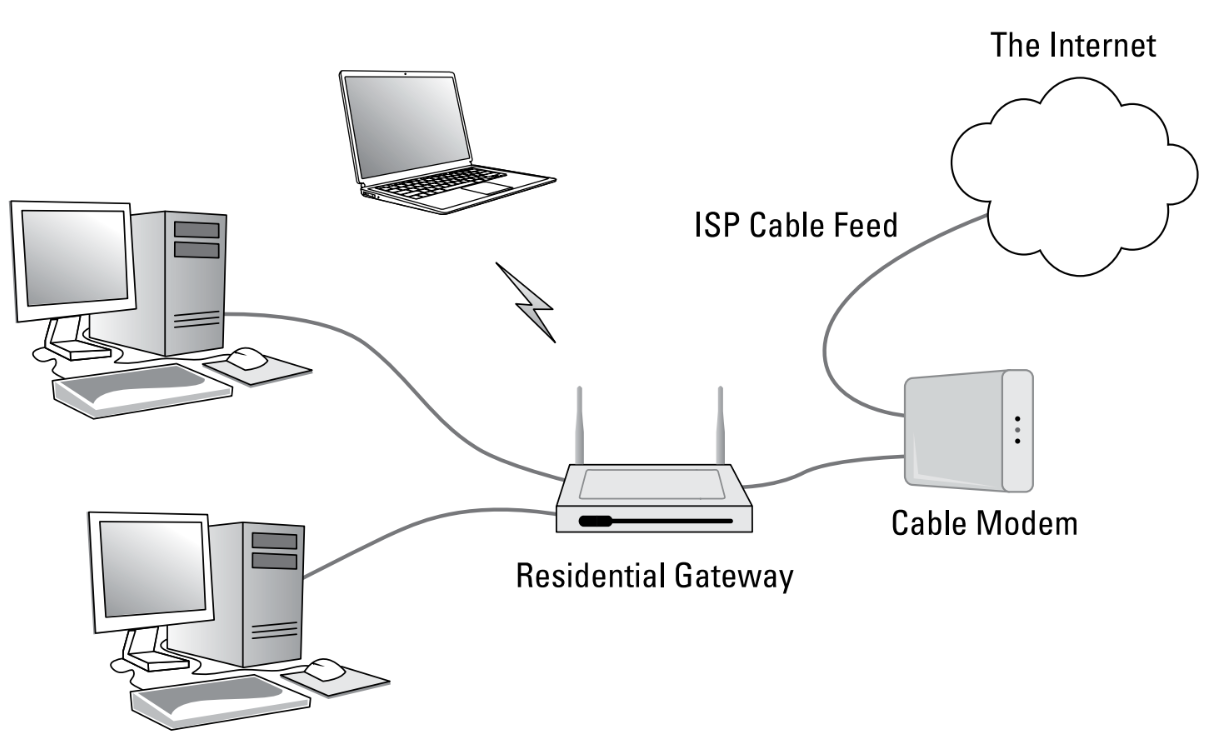
\includegraphics[width=0.8\textwidth]{fig/fig33}
	\caption{De vigtigste parametre for et datakommunikationskabel som lavpasfilter}
	\label{fig:low_pass_filter}
\end{figure}

\section{Fiberoptik}
Fiberoptiske kabler bruges normalt til at overføre digitale signaler over lange afstande med høj båndbredde. De har en kerne af rent optisk glas omgivet af en optisk kappe, der guider lysimpulser gennem kablet. Fiberoptik er mindre modtagelige for EMI og har en større informationsbærende kapacitet end kobberkabler.

\begin{figure}[h!]
	\centering
	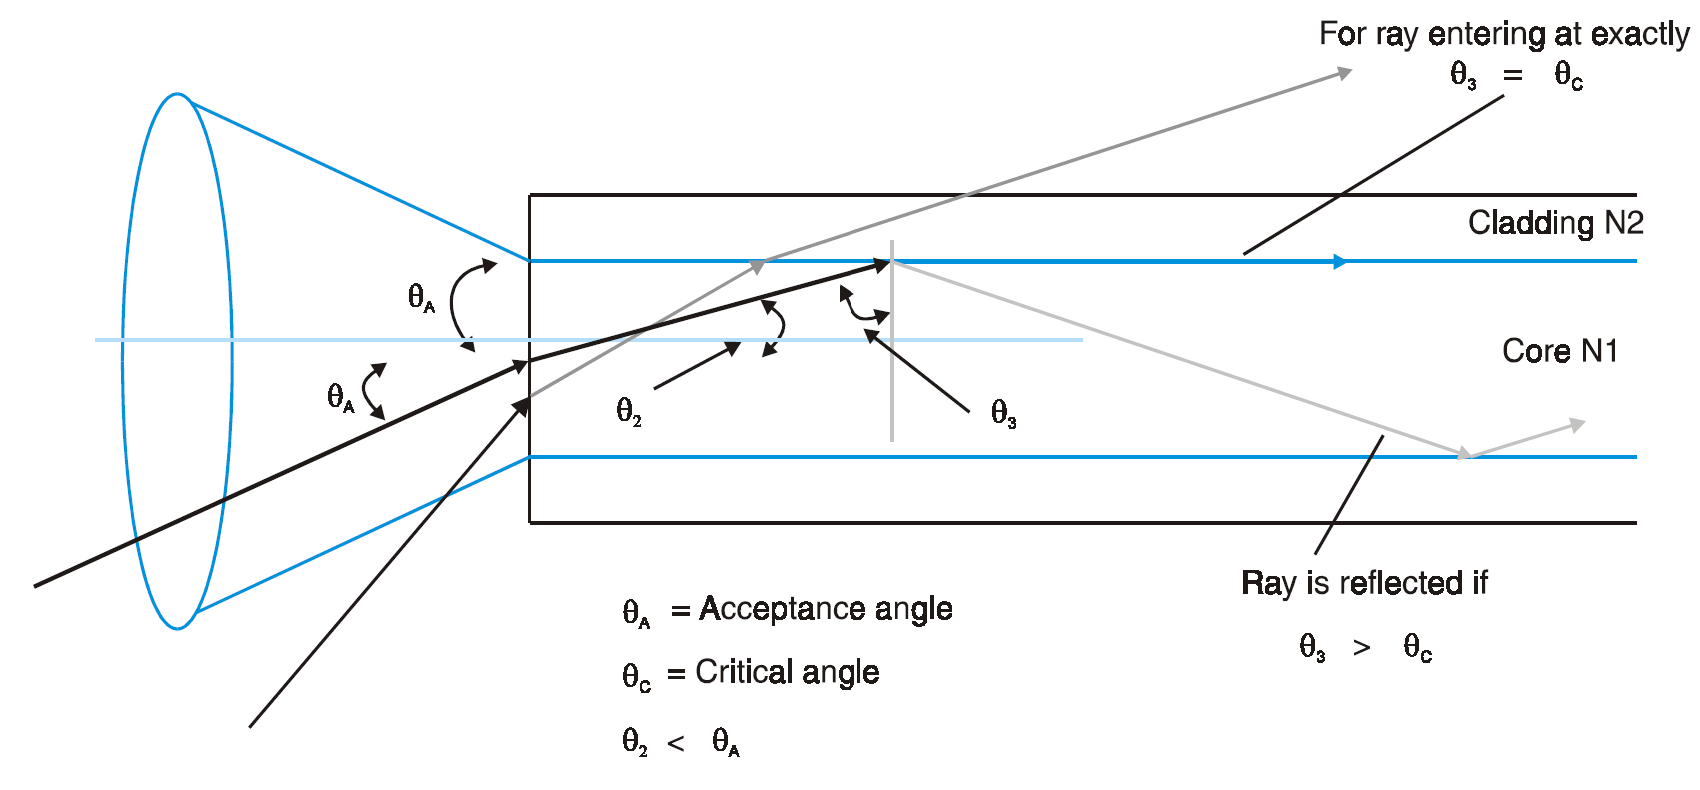
\includegraphics[width=0.8\textwidth]{fig/fig34}
	\caption{Opbygning af et fiberoptisk kabel}
	\label{fig:fiber_optic}
\end{figure}

\subsection{Driftsteori for fiberoptik}
Kommunikation over fiberoptiske kabler fungerer på princippet om, at lys bevæger sig gennem forskellige medier med forskellige hastigheder (på samme måde som radiobølger). Når lys bevæger sig fra et medium med en bestemt densitet til et andet med en anden densitet, ændrer lyset retning. Dette fænomen kaldes brydning.

\[
n = \frac{\text{Lysets hastighed i vakuum}}{\text{Lysets hastighed i mediet}}
\]

I et typisk fiberoptisk medium bevæger lyset sig ved cirka \(2 \times 10^8\) m/s. Brydningsindekset er derfor:

\[
n_1 = \frac{3 \times 10^8}{2 \times 10^8} = 1.5
\]

\begin{figure}[h!]
	\centering
	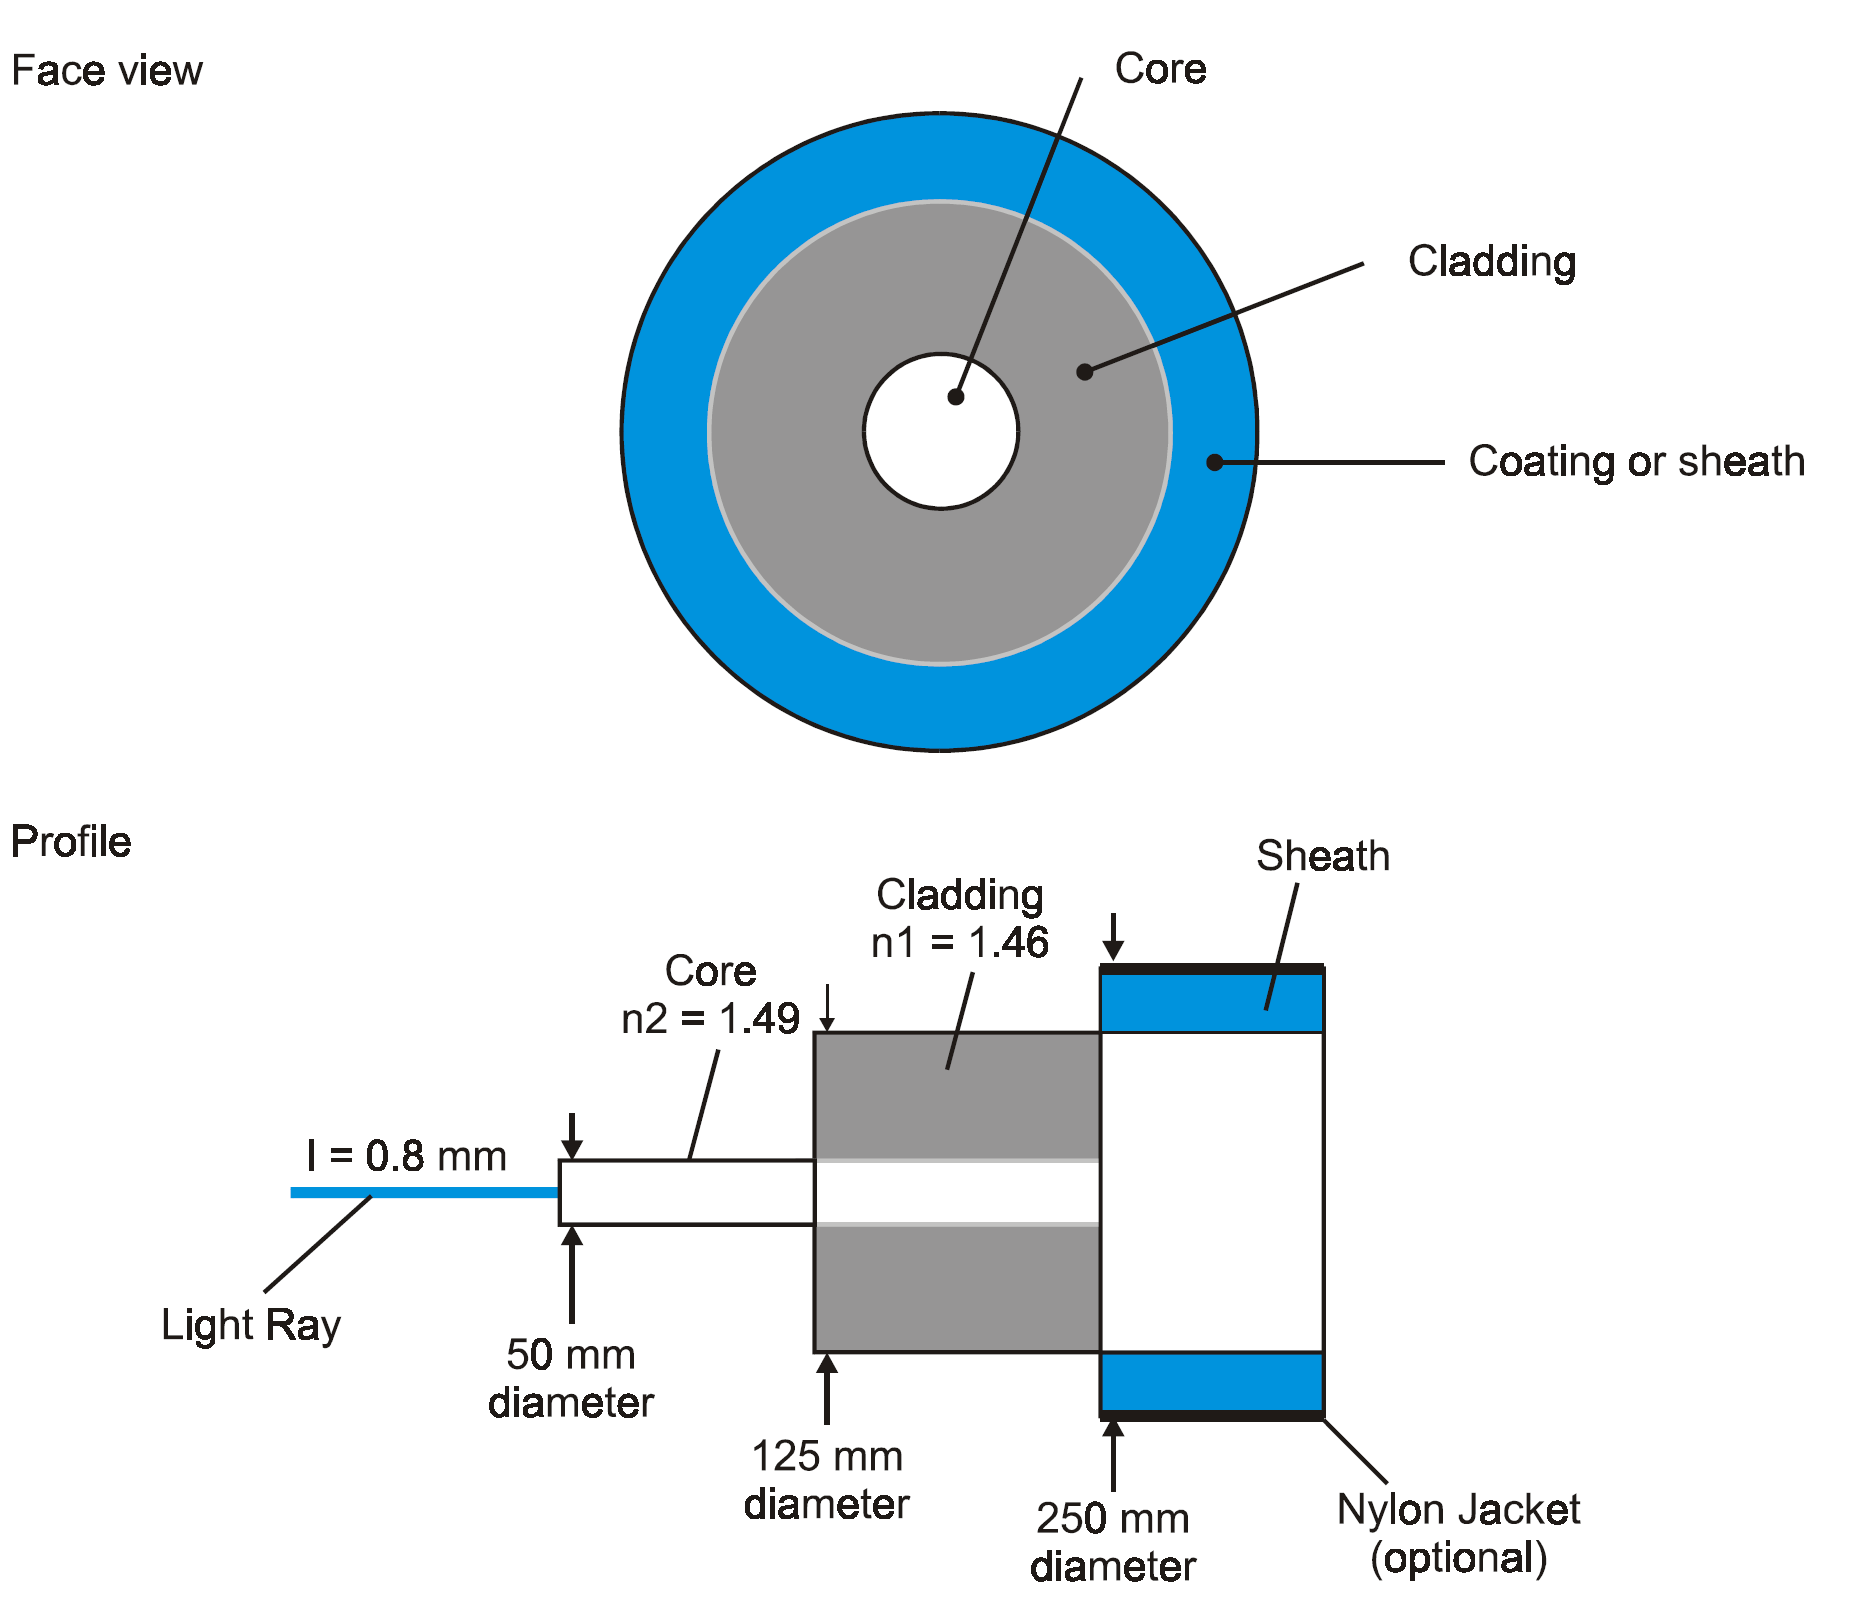
\includegraphics[width=0.7\textwidth]{fig/fig35}
	\caption{Optisk fiber principper}
	\label{fig:optical_fiber_principles}
\end{figure}

Den optiske fiber fungerer som en bølgeleder (eller lysleder) for lysimpulser genereret af en lyskilde. Lyskilden er typisk en laserdiode eller lysdiode (LED), der opererer ved bølgelængder på 0.85, 1.3 eller 1.55 mikrometer.

\begin{figure}[h!]
	\centering
	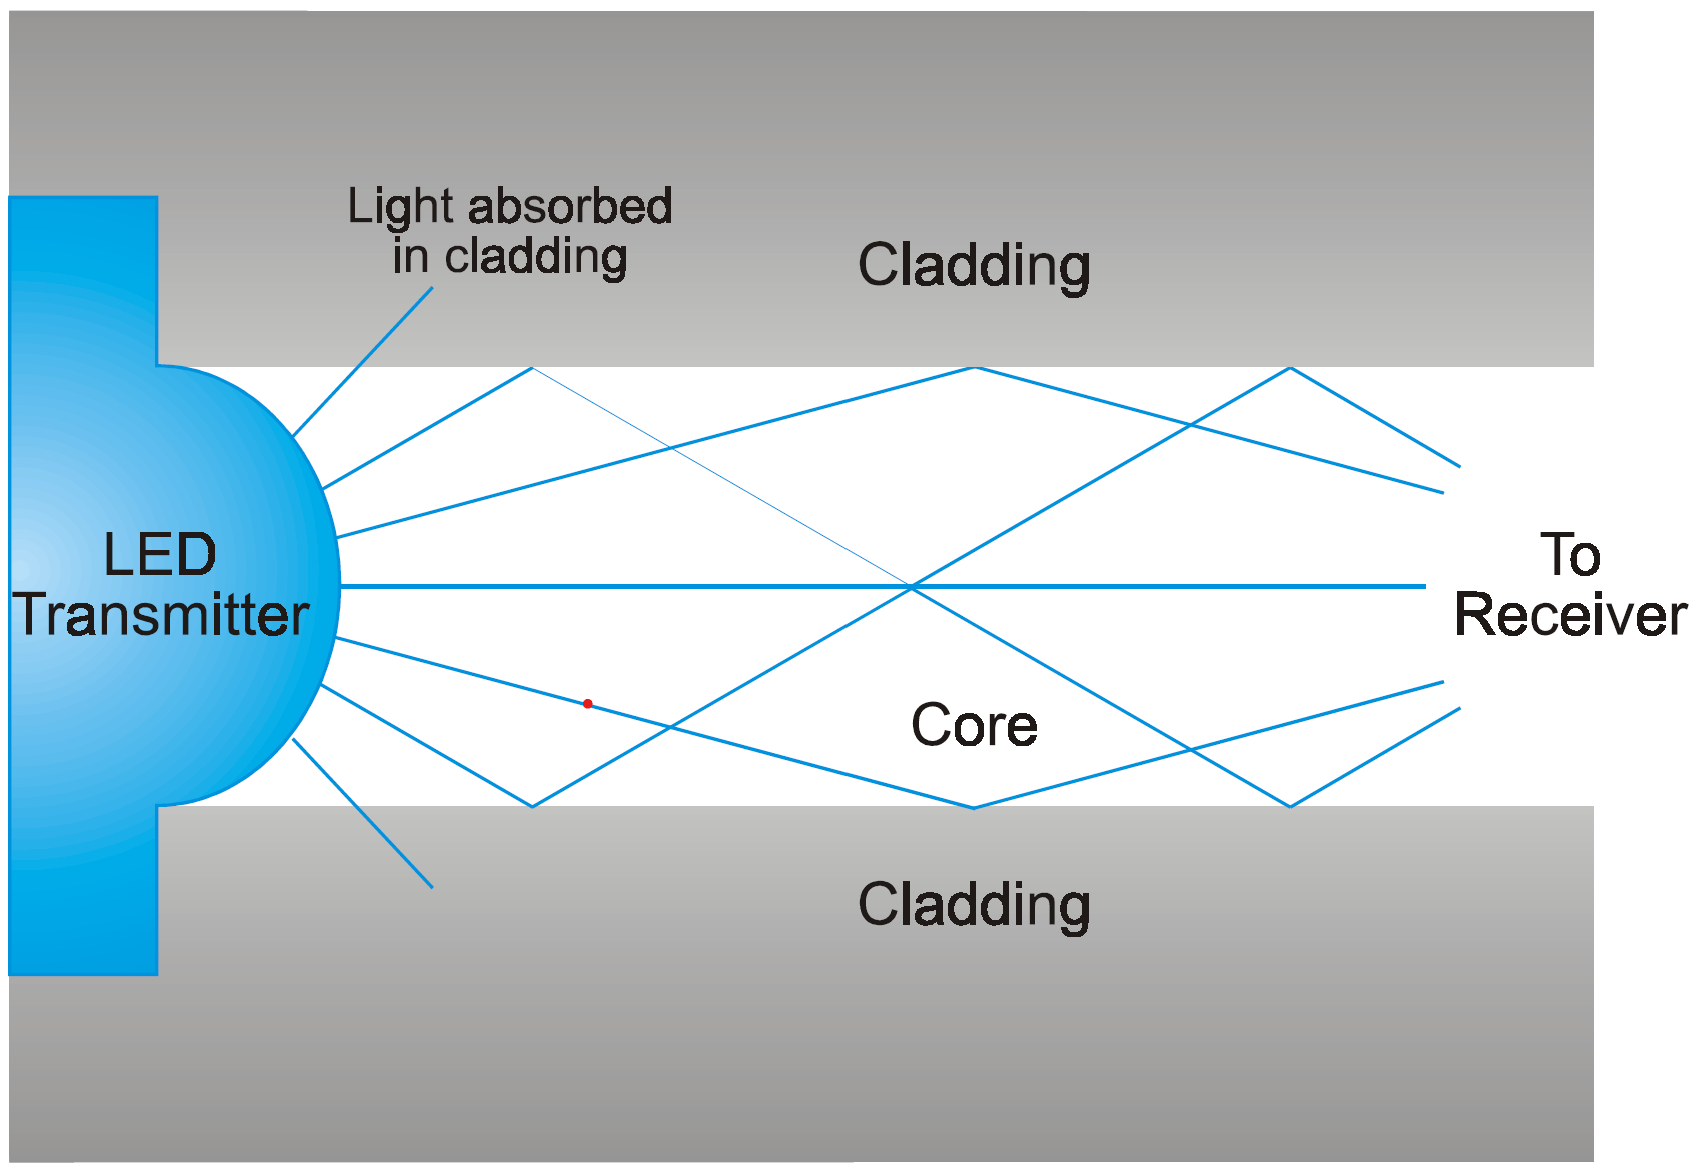
\includegraphics[width=0.6\textwidth]{fig/fig36}
	\caption{LED-lyskilde koblet til en multimode fiber (Step Index)}
	\label{fig:led_fiber}
\end{figure}

\subsection{Installation og vedligeholdelse}
Når Ethernet-kabler installeres, er det vigtigt at følge producentens specifikationer og industristandarder for at sikre korrekt ydeevne. Dette inkluderer korrekt bøjning af kabler, undgåelse af skarpe vinkler, og sikring af gode forbindelser i stik og patch paneler.
\newline
\newline
\noindent Vedligeholdelse af Ethernet-kabler omfatter regelmæssig inspektion for skader, sikring af korrekte forbindelser og opdatering af kablingsinfrastrukturen efter behov.

\subsection{Forbindelsestyper og Stik}
En korrekt installation af Ethernet-kabler inkluderer også valg af passende stik og forbindelsestyper. De mest almindelige typer af stik omfatter:
\begin{itemize}
	\item \textbf{RJ45-stik:} Det mest anvendte stik til Ethernet-forbindelser. RJ45-stik har otte ledere og bruges til at forbinde twisted pair kabler til netværksenheder som computere, routere og switches.
	\item \textbf{Andre stiktyper:} I specifikke applikationer kan andre stiktyper som RJ11, DB9, eller specialiserede industrielle stik være nødvendige.
\end{itemize}

\subsection{Ydeevne og Hastigheder}
Ydeevnen af Ethernet-kabler afhænger af kabeltypen og dens specifikationer:
\begin{itemize}
	\item \textbf{Hastighedskategorier:} Forskellige kategorier af twisted pair kabler (f.eks. Cat5e, Cat6, Cat6a, Cat7) tilbyder varierende niveauer af ydeevne i forhold til båndbredde og hastighed.
	\item \textbf{Maksimal Kabellængde:} For hver kategori af kabel er der en maksimal anbefalet kabellængde, som påvirker netværkets ydeevne. For eksempel er maksimal længde for Cat5e og Cat6 kabler 100 meter.
\end{itemize}

\subsection{Standarder og Protokoller}
Ethernet-netværk styres af en række standarder og protokoller, der sikrer kompatibilitet og ydeevne:
\begin{itemize}
	\item \textbf{IEEE 802.3:} Denne standard dækker de fleste aspekter af Ethernet-netværk og inkluderer specifikationer for forskellige hastigheder og medier.
	\item \textbf{Power over Ethernet (PoE):} PoE tillader samtidig overførsel af data og strøm via samme kabel, hvilket er nyttigt til enheder som IP-kameraer og trådløse adgangspunkter.
\end{itemize}

\subsection{Fejlfinding og Vedligeholdelse}
Regelmæssig vedligeholdelse og fejlfinding er afgørende for at opretholde et pålideligt Ethernet-netværk:
\begin{itemize}
	\item \textbf{Typiske Problemer og Løsninger:} Almindelige problemer inkluderer kabelbrud, dårlige forbindelser og interferens. Korrekt terminering og regelmæssig inspektion kan afhjælpe mange af disse problemer.
	\item \textbf{Testudstyr:} Kabeltestere og certificeringsværktøjer er vigtige for at verificere kabelintegritet og ydeevne. Disse værktøjer kan identificere problemer som krydsede par, åben kredsløb, og interferens.
\end{itemize}

\section{EMC (Elektromagnetisk Kompatibilitet)}
Elektromagnetisk kompatibilitet (EMC) er afgørende for at sikre, at elektroniske enheder og systemer kan fungere korrekt uden at forstyrre eller blive forstyrret af elektromagnetiske felter. I forbindelse med Ethernet-kabling er EMC vigtigt for at forhindre interferens, som kan påvirke signalintegriteten og netværkets ydeevne.
\begin{itemize}
	\item \textbf{Skærmning:} Shielded twisted pair (STP) kabler og korrekt jordforbindelse hjælper med at reducere EMI og forbedre EMC.
	\item \textbf{Kabelruting:} Undgå at placere Ethernet-kabler tæt på strømkabler eller andre kilder til elektromagnetisk støj.
	\item \textbf{Filter og Beskyttelse:} Brug af filtrerings- og beskyttelsesmekanismer kan hjælpe med at beskytte netværksenheder mod EMI.
\end{itemize}

\subsection{Sikkerhed og ydeevne}
Sikkerhed og ydeevne er afgørende faktorer ved installation af Ethernet-kabler i industrielle miljøer. Korrekt jordforbindelse og afskærmning skal implementeres for at beskytte mod EMI. Derudover skal kablerne være i stand til at opretholde datahastigheder og pålidelighed under alle driftsforhold.
\newline\newline\noindent 
Ved at følge disse retningslinjer kan en pålidelig og effektiv 
\newline\noindent Ethernet-netværksinfrastruktur etableres, som kan modstå de udfordringer, der findes i industrielle miljøer.

\chapter{Hardware Konfigurationer}
\section{Switch}
\section{Router}

	% Industrielt netværk
	\part{Industrielt Netværk}
\chapter{Introduktion til Industrielle Netværk}
\label{chapter:introduktion_industrielle_netværk}
\section{Hvad er Industrielt Netværk?}
Industrielle netværk refererer til kommunikationssystemer designet specifikt til at forbinde enheder i industrielle miljøer som fabrikker, produktionsanlæg og andre automatiserede systemer. Disse netværk muliggør dataudveksling mellem forskellige maskiner og kontrolsystemer, hvilket optimerer produktionsprocesser, forbedrer effektiviteten og øger pålideligheden.

\subsection{Historisk Udvikling af Netværk i Industrien}
Industrielle netværk har gennemgået en betydelig udvikling over tid. I begyndelsen blev industrielle kontrolsystemer typisk isolerede og brugte proprietære kommunikationsprotokoller. Med fremkomsten af standardiserede protokoller og netværksteknologier som Ethernet og TCP/IP, er det blevet muligt at integrere industrielle netværk med virksomhedens IT-systemer, hvilket har ført til mere sammenhængende og fleksible produktionsmiljøer.

\subsection{Tidlige Industrielle Netværk}
I de tidlige dage af industriel automatisering var kommunikationssystemer ofte punkt-til-punkt forbindelser, hvor hver enhed var direkte forbundet med kontrolsystemet. Dette resulterede i komplekse og dyre installationer, der var svære at vedligeholde og udvide.

\subsection{Overgang til Standardiserede Protokoller}
Med introduktionen af standardiserede protokoller som Modbus og PROFIBUS i 1980'erne, blev det muligt at oprette mere fleksible og skalerbare netværk. Disse protokoller gjorde det lettere at forbinde enheder fra forskellige producenter og reducere kompleksiteten i installationsprocessen.

\subsection{Integration med Ethernet og IT-Systemer}
I 1990'erne og 2000'erne begyndte industrielle netværk at integrere Ethernet-teknologi, hvilket gjorde det muligt at udnytte de højere hastigheder og den større båndbredde, som Ethernet tilbyder. Dette førte til udviklingen af industri-specifikke Ethernet-protokoller som EtherNet/IP, PROFINET og Modbus TCP. Integration med IT-systemer har desuden gjort det muligt for virksomheder at implementere Industri 4.0-konceptet, hvor produktionsdata kan analyseres i realtid for at optimere driften.

\subsection{Nutidige og Fremtidige Trends}
I dag fortsætter industrielle netværk med at udvikle sig med fokus på trådløse teknologier, cybersikkerhed og Internet of Things (IoT). Fremtidige trends omfatter brugen af 5G til industriel kommunikation, øget brug af kunstig intelligens til netværksovervågning og vedligeholdelse samt integration af avancerede sensorer og aktuatorer for at forbedre produktionsprocesser.

\subsection{Betydningen af Industrielle Netværk}
Industrielle netværk spiller en afgørende rolle i moderne produktionsmiljøer ved at:
\begin{itemize}
	\item \textbf{Forbedre Effektiviteten:} Automatisering og realtidsdataudveksling mellem maskiner og kontrolsystemer optimerer produktionsprocesser og reducerer nedetid.
	\item \textbf{Øge Pålideligheden:} Standardiserede protokoller og robuste netværksdesigns sikrer pålidelig kommunikation selv i krævende industrielle miljøer.
	\item \textbf{Muliggøre Fleksibilitet:} Skalerbare netværk gør det nemmere at tilpasse sig ændringer i produktionskrav og integrere nye teknologier uden omfattende ændringer i infrastrukturen.
	\item \textbf{Styrke Sikkerheden:} Avancerede sikkerhedsprotokoller og netværksovervågning beskytter mod cybertrusler og uautoriseret adgang.
\end{itemize}

\chapter{Protokoller og Elektriske Standarder}

\section{Introduktion til Protokoller og Elektriske Standarder}
I industrielle netværk spiller både netværksprotokoller og elektriske standarder en afgørende rolle for at sikre effektiv og pålidelig kommunikation. Selvom disse to begreber ofte nævnes sammen, tjener de forskellige formål og adresserer forskellige aspekter af datakommunikation. Det er derfor vigtigt at forstå deres forskelle og hvordan de komplementerer hinanden.

\section{Netværksprotokoller: Reglerne for Kommunikation}
En netværksprotokol kan sammenlignes med et sprog eller en samtaleetikette, som alle deltagere i en samtale skal følge for at kunne forstå hinanden. Ligesom mennesker har brug for et fælles sprog for at kommunikere effektivt, kræver netværksenheder en fælles protokol for at udveksle data korrekt. En netværksprotokol definerer de regler og konventioner, som netværksenheder skal følge, herunder hvordan data pakkes, adresseres, transmitteres, modtages og behandles.

\subsection{Analogier for at Forstå Netværksprotokoller}
For at forstå netværksprotokoller kan vi bruge analogien med en samtale mellem mennesker. Tænk på netværksprotokollen som de regler, der dikterer, hvordan en samtale skal foregå for at sikre, at begge parter forstår hinanden:

\begin{itemize}
	\item \textbf{Start af Kommunikation:} Ligesom en samtale begynder med en hilsen, starter en netværksforbindelse ofte med en \texttt{TCP connection request}, hvor en enhed anmoder om at etablere en forbindelse. Modparten svarer med en \texttt{TCP connection reply} for at bekræfte.
	\item \textbf{Udveksling af Information:} Under samtalen udveksler parterne information, som spørgsmål og svar, f.eks. "Got the time?" og "2:00". I en netværkskommunikation kunne dette svare til udveksling af data, hvor en enhed sender en kommando, og den anden enhed reagerer med den ønskede information.
	\item \textbf{Afslutning:} Når samtalen er færdig, kan den ene person sige "farvel," ligesom en netværksforbindelse afsluttes ved, at begge parter signalerer, at de er færdige med kommunikationen.
\end{itemize}

\begin{figure}[h]
	\centering
	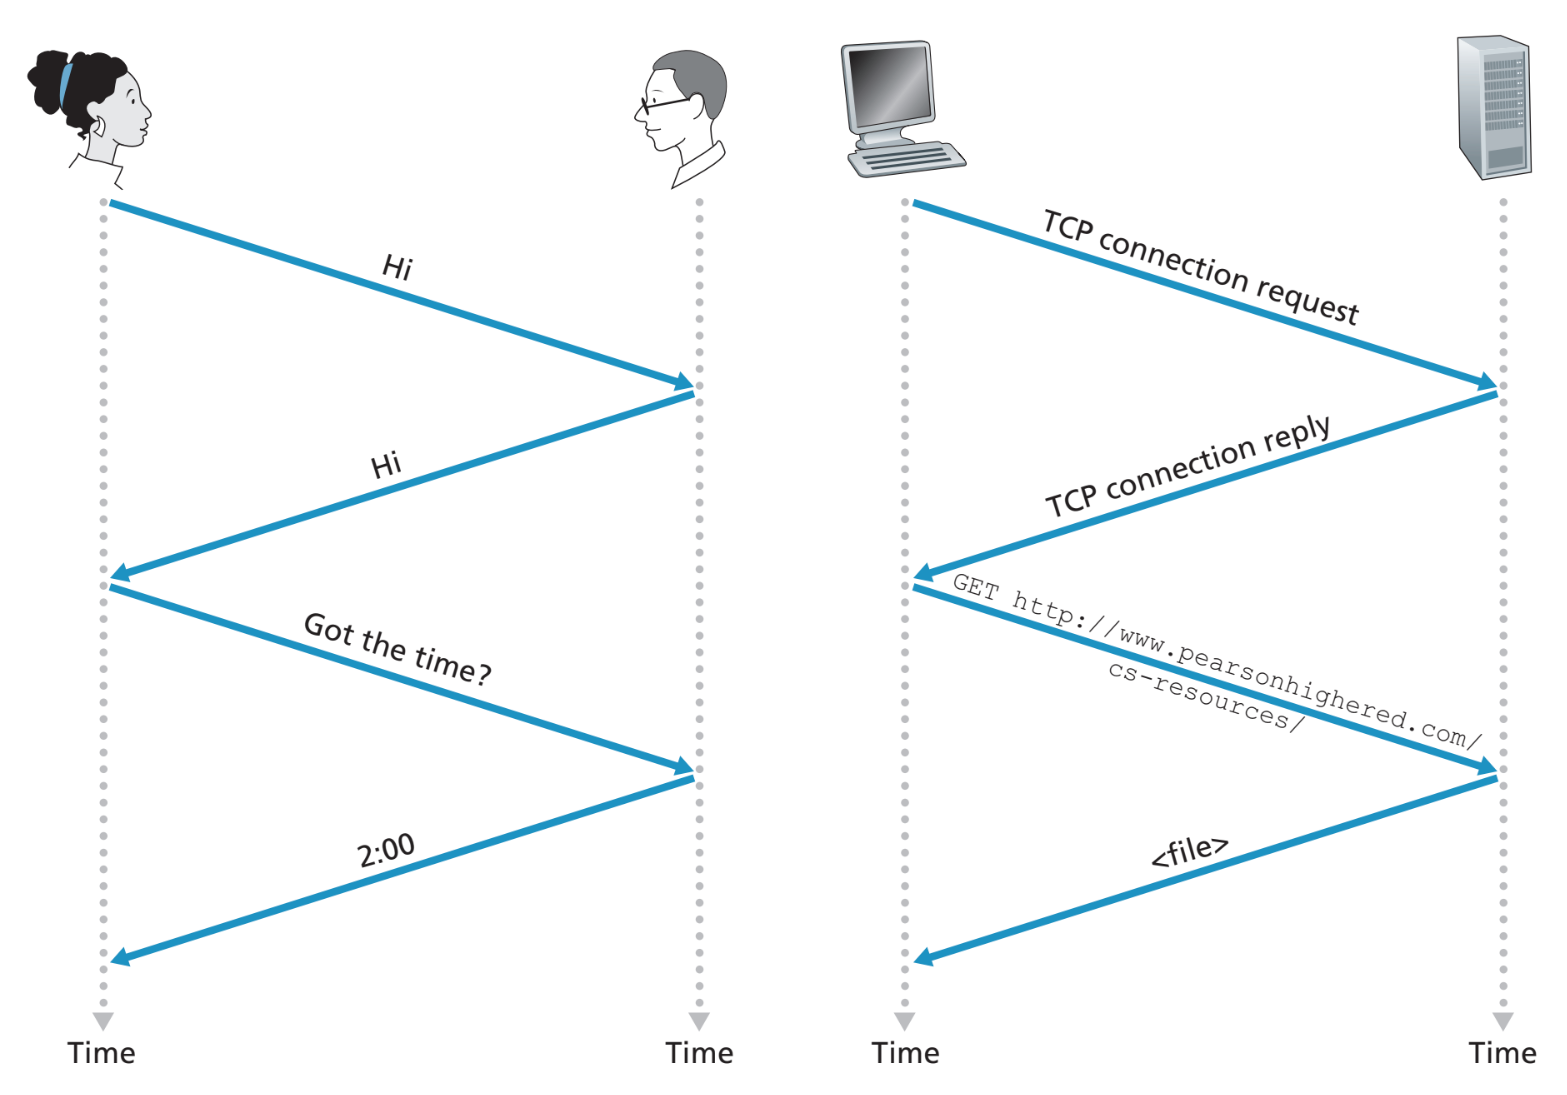
\includegraphics[width=\textwidth]{fig/fig42.png}
	\caption{Sammenligning mellem en menneskelig samtale og en TCP-forbindelse}
	\label{fig:tcp-analogy}
\end{figure}
\noindent Billedet i figur \ref{fig:tcp-analogy} illustrerer, hvordan en sådan kommunikation foregår, både mellem mennesker og i en netværksprotokol som TCP. Denne visuelle analogi hjælper med at forstå, hvordan protokoller sikrer, at begge parter i en netværkskommunikation forstår hinanden korrekt og pålideligt.
\newline\newline\noindent
Eksempler på almindelige netværksprotokoller i industrielle netværk inkluderer Ethernet/IP, Profinet, og Modbus TCP. Disse protokoller muliggør pålidelig kommunikation mellem forskellige enheder såsom PLC'er, sensorer, og aktuatorer i et automatiseret miljø.

\section{Elektriske Standarder: Den Fysiske Infrastruktur}
Mens netværksprotokoller styrer, hvordan data kommunikeres, beskriver elektriske standarder de fysiske egenskaber og specifikationer for, hvordan data transmitteres over et medie. Dette inkluderer alt fra typen af kabler og stik, til spændingsniveauer og frekvenser, der anvendes under transmissionen.

\subsection{Analogier for at Forstå Elektriske Standarder}
Vi kan forstå elektriske standarder ved at sammenligne dem med jernbanespor:

\begin{itemize}
	\item \textbf{Sporbredde:} Ligesom tog skal køre på skinner med en bestemt bredde, skal data overføres gennem kabler med specifikke fysiske egenskaber. Standarderne specificerer, hvilken type kabler (f.eks. kobber eller fiberoptik) og stik der skal bruges.
	\item \textbf{Sikkerhed og Pålidelighed:} Elektriske standarder sikrer, at dataoverførslen er sikker og pålidelig ved at specificere grænser for elektrisk støj og spænding. Dette kan sammenlignes med sikkerhedsforanstaltninger på jernbanen, der forhindrer ulykker og sikrer, at togene kører uden afbrydelser.
	\item \textbf{Båndbredde:} Ligesom jernbanesystemer har kapacitet til at transportere et bestemt antal tog per tidsenhed, dikterer elektriske standarder også, hvor hurtigt data kan overføres og hvor meget information der kan transporteres samtidigt.
\end{itemize}
\noindent
Eksempler på elektriske standarder omfatter RS-232, RS-485, og IEEE 802.3 (Ethernet-standarder). Disse standarder definerer de fysiske parametre, såsom kabeltype og stik, der er nødvendige for at sikre kompatibilitet og pålidelighed i datatransmissionen.

\section{Eksempel på Samspil mellem Protokoller og Elektriske Standarder}
Lad os overveje en situation, hvor en industriel robotarm kommunikerer med en kontrolstation over et netværk. Netværksprotokollen, såsom Profinet, styrer, hvordan data om robotarmens position og status sendes til kontrolstationen og tilbage. Den elektriske standard, såsom Ethernet (IEEE 802.3), bestemmer, hvilken type kabler og stik der bruges, samt de fysiske transmissionsparametre, der sikrer, at dataene overføres korrekt og pålideligt.
\newline\newline\noindent
I denne situation fungerer netværksprotokollen som "sproget", som enhederne bruger til at "tale" med hinanden, mens den elektriske standard fungerer som "infrastrukturen", der gør det muligt for denne kommunikation at finde sted. Begge er nødvendige for at sikre en problemfri og effektiv drift af det industrielle netværk.

\section{Opsummering: Forskellen mellem Protokoller og Elektriske Standarder}
Selvom både netværksprotokoller og elektriske standarder er afgørende for effektiv datakommunikation i industrielle netværk, tjener de forskellige formål:

\begin{itemize}
	\item \textbf{Netværksprotokoller:} Disse styrer, hvordan data pakkes, sendes, modtages, og behandles mellem enheder på et netværk. De skaber et fælles sprog, som alle enheder i netværket forstår, og sikrer, at informationen overføres korrekt.
	
	\item \textbf{Elektriske Standarder:} Disse definerer de fysiske parametre for datatransmissionen, herunder kabeltyper, spændingsniveauer og forbindelsesmåder. De sikrer, at de tekniske aspekter af dataoverførslen er sikre og pålidelige, hvilket muliggør kompatibilitet mellem forskellige enheder og systemer.
\end{itemize}
\noindent Protokollerne kan ses som de "regler" og "sprog", som enhederne i netværket bruger til at kommunikere, mens de elektriske standarder er den "infrastruktur", der muliggør, at denne kommunikation kan foregå sikkert og effektivt. For at opnå en robust industriel netværksløsning er det nødvendigt at anvende både passende protokoller og elektriske standarder i designet og implementeringen.

\chapter{Netværkstopologi}
\begin{figure}[!h]
	\centering
	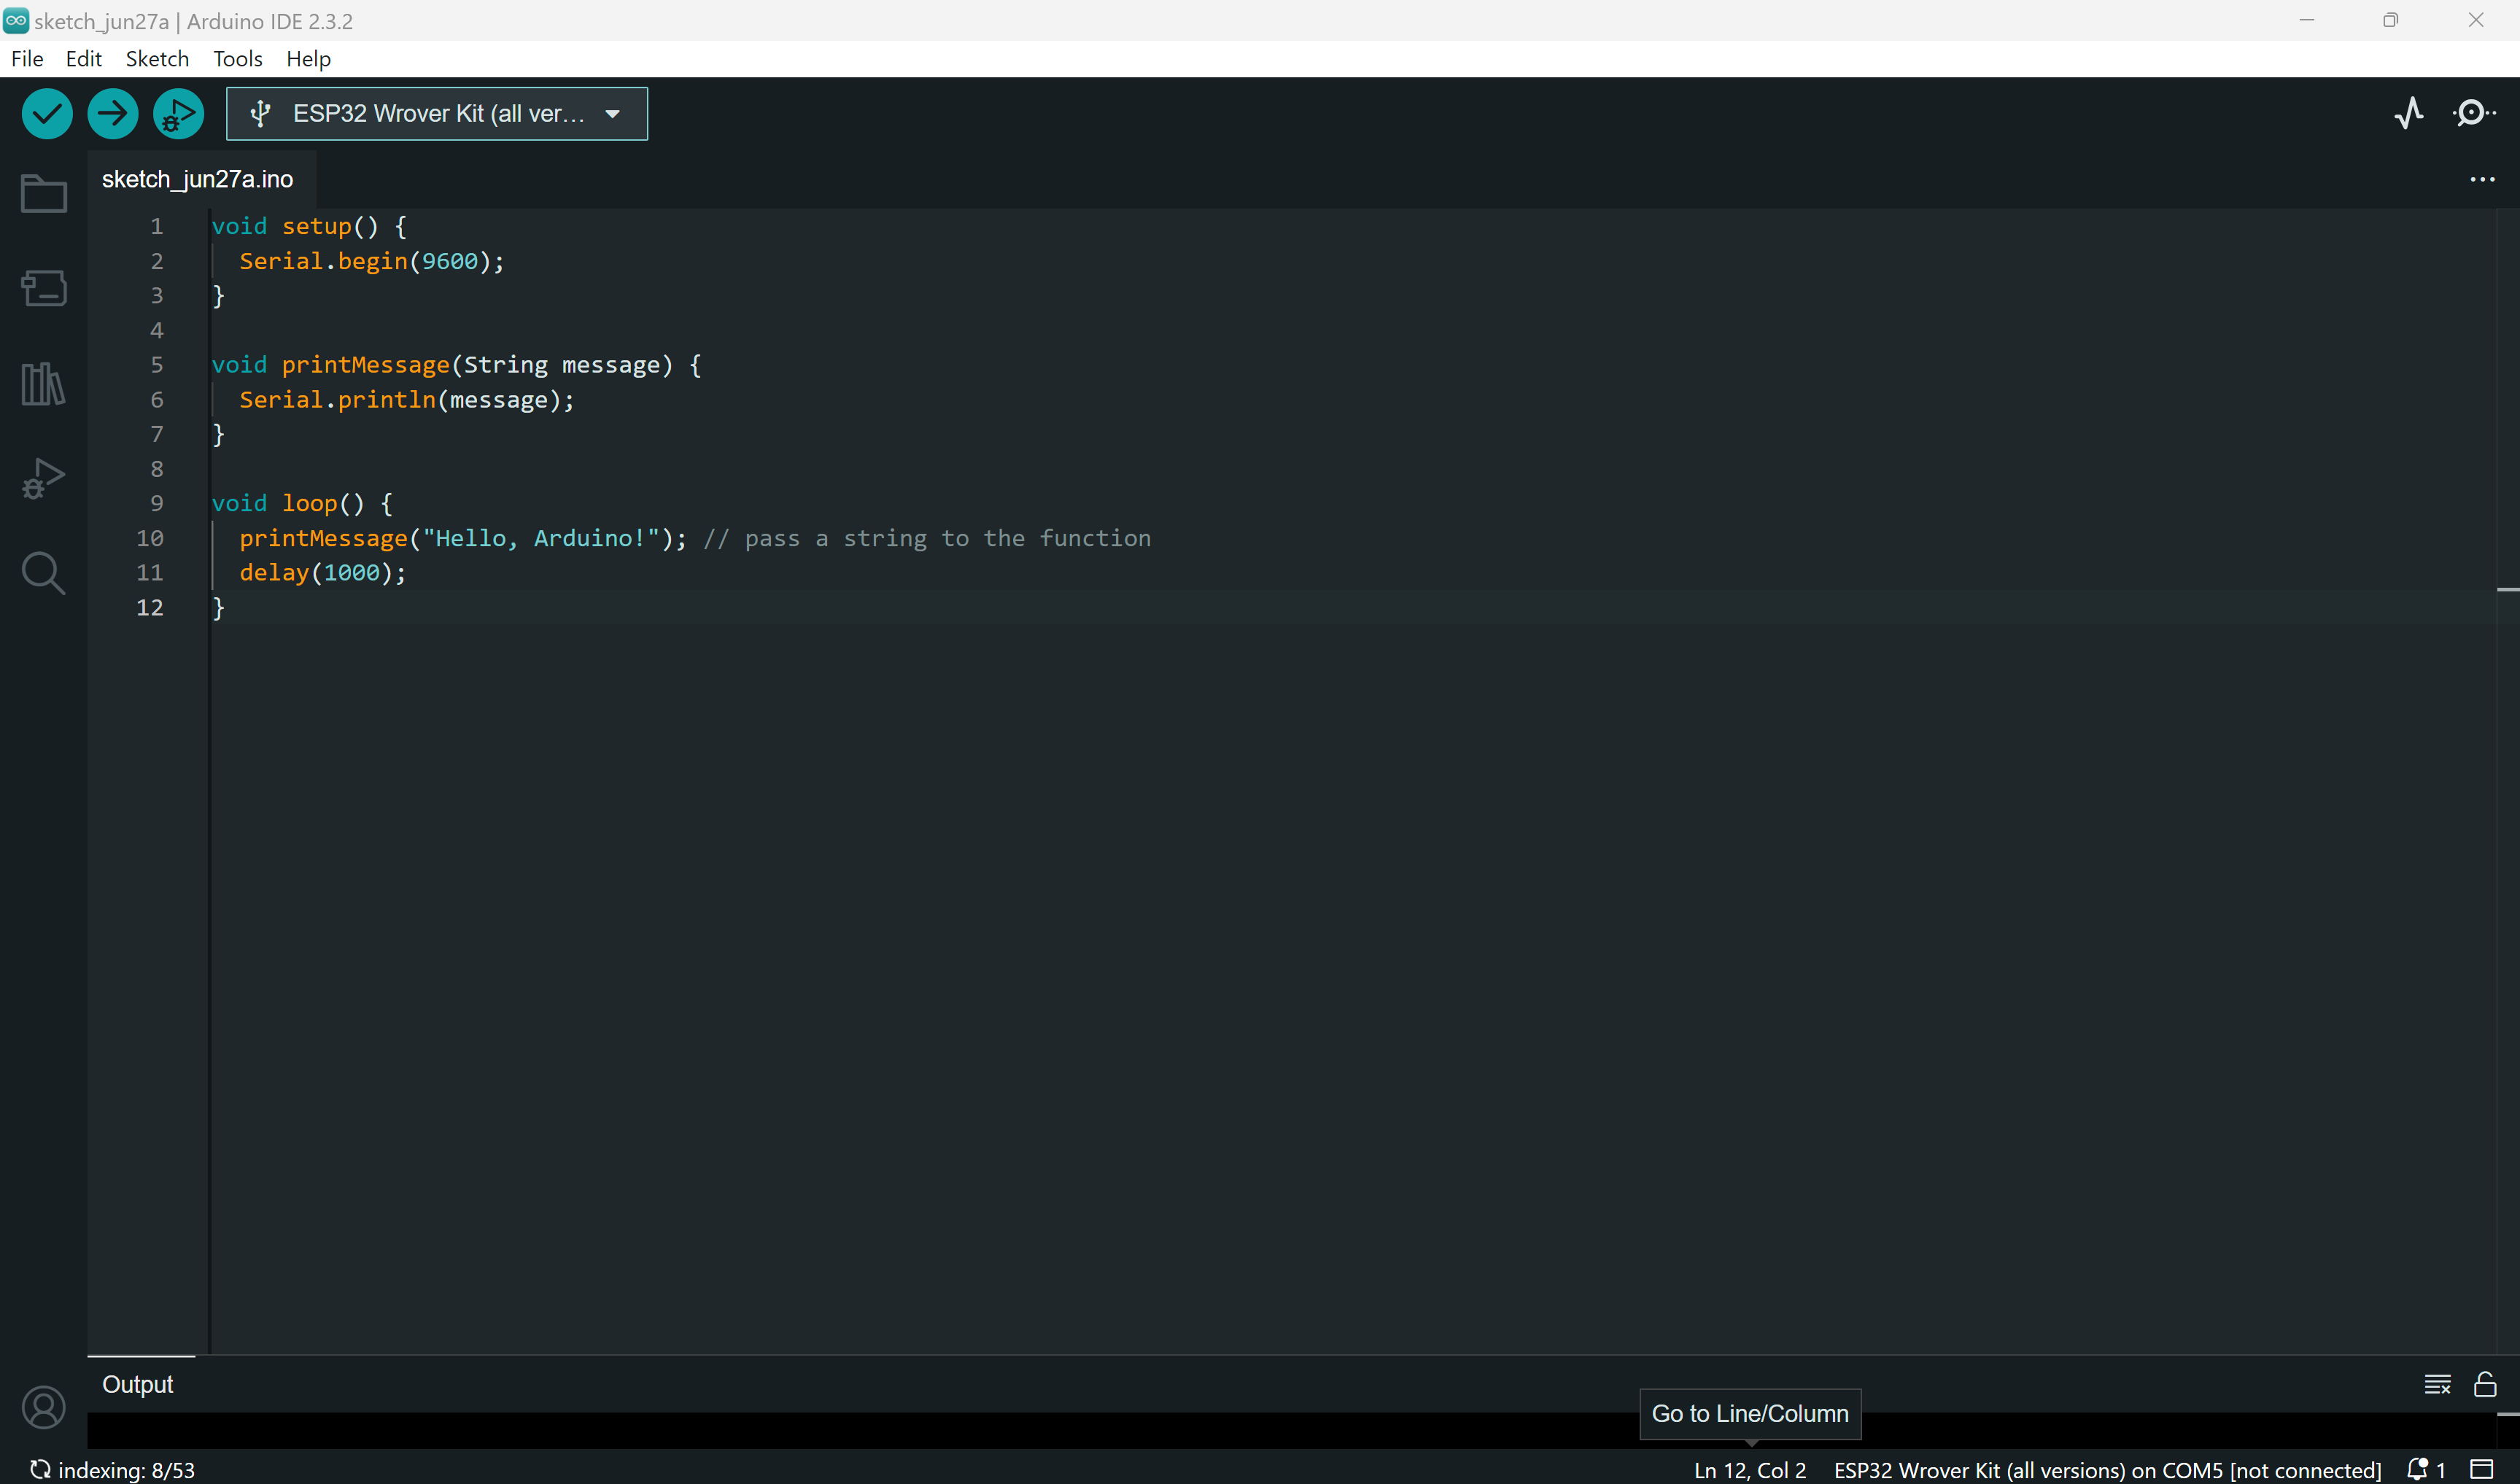
\includegraphics[width=\linewidth]{fig/fig12.png}
	\caption{Netværkstopologi}
\end{figure}
\noindent Netværkstopologi refererer til arrangementet og layoutet af noder og forbindelser i et netværk. Det beskriver både den fysiske og logiske struktur af netværket. Der er flere forskellige typer af topologier, hver med sine egne fordele og ulemper. Nedenfor gennemgås de mest almindelige netværkstopologier:

\section{Punkt-til-punkt Topologi}
I en punkt-til-punkt topologi er to noder direkte forbundet til hinanden. Denne type topologi bruges ofte i situationer, hvor en direkte forbindelse mellem to enheder er nødvendig.
\begin{itemize}
	\item \textbf{Fordele:}
	\begin{itemize}
		\item Meget enkel og hurtig forbindelse.
		\item Lav latenstid og høj båndbredde.
	\end{itemize}
	\item \textbf{Ulemper:}
	\begin{itemize}
		\item Ikke skalerbar; kun egnet til små netværk.
		\item Hvis forbindelsen fejler, går kommunikationen tabt.
	\end{itemize}
\end{itemize}

\section{Bustopologi}
I en bustopologi er alle noder forbundet til en enkelt kommunikationslinje eller bus. Dataene, der sendes af en node, rejser langs bussen og kan modtages af alle noderne.
\begin{itemize}
	\item \textbf{Fordele:}
	\begin{itemize}
		\item Nem og billig at installere.
		\item Kræver mindre kabel end en stjernetopologi.
	\end{itemize}
	\item \textbf{Ulemper:}
	\begin{itemize}
		\item Svært at fejlfinde og identificere problemer.
		\item Begrænset kabel længde og antal noder.
		\item Hvis hovedkabel fejler, går hele netværket ned.
	\end{itemize}
\end{itemize}

\section{Ringtopologi}
I en ringtopologi er noderne forbundet i en cirkulær rækkefølge. Hver node har præcis to naboer, og data bevæger sig i én retning (eller i nogle tilfælde i begge retninger) langs ringen.
\begin{itemize}
	\item \textbf{Fordele:}
	\begin{itemize}
		\item Dataoverførsel er relativt hurtig, da data bevæger sig i en bestemt retning.
		\item Ingen kollisionsdomæner som i bustopologi.
	\end{itemize}
	\item \textbf{Ulemper:}
	\begin{itemize}
		\item En fejl i en enkelt node eller forbindelse kan påvirke hele netværket.
		\item Mere kompleks at installere og konfigurere.
	\end{itemize}
\end{itemize}

\section{Stjernetopologi}
I en stjernetopologi er alle noder forbundet til en central hub eller switch. Hubben fungerer som en repeater for dataene, hvilket betyder, at data, der sendes fra en node, først sendes til hubben og derefter videre til den destination, der er tiltænkt.
\begin{itemize}
	\item \textbf{Fordele:}
	\begin{itemize}
		\item Enkel at installere og administrere.
		\item Fejl i en enkelt kabel påvirker ikke resten af netværket.
		\item Let at tilføje eller fjerne noder uden at forstyrre netværket.
	\end{itemize}
	\item \textbf{Ulemper:}
	\begin{itemize}
		\item Hvis central hub fejler, går hele netværket ned.
		\item Kræver mere kabel end nogle andre topologier.
	\end{itemize}
\end{itemize}

\section{Trætopologi}
Trætopologi, også kendt som hierarkisk topologi, er en hybrid topologi, der kombinerer egenskaberne af stjernetopologi og bustopologi. Den består af grupper af stjernetopologier, der er forbundet til et bus-lignende backbone-kabel.
\begin{itemize}
	\item \textbf{Fordele:}
	\begin{itemize}
		\item Udvidelsesvenlig og let at administrere.
		\item Fejl i en enkelt node påvirker ikke hele netværket.
	\end{itemize}
	\item \textbf{Ulemper:}
	\begin{itemize}
		\item Mere kompleks at konfigurere end en simpel stjerne- eller bustopologi.
		\item Backbone-kablet er et enkelt fejlpunkt.
	\end{itemize}
\end{itemize}

\section{Masketopologi}
I en masketopologi er hver node forbundet til flere andre noder, hvilket skaber et netværk af forbindelser. Dette kan være en fuld mesh, hvor alle noder er forbundet til hinanden, eller en delvis mesh, hvor nogle noder kun er forbundet til nogle få andre noder.
\begin{itemize}
	\item \textbf{Fordele:}
	\begin{itemize}
		\item Meget pålidelig, da flere forbindelser sikrer, at data kan tage alternative ruter.
		\item Fejl i en enkelt forbindelse påvirker ikke hele netværket.
	\end{itemize}
	\item \textbf{Ulemper:}
	\begin{itemize}
		\item Meget dyrt og komplekst at installere og vedligeholde.
		\item Kræver mange kabler og porte.
	\end{itemize}
\end{itemize}

\section{Hybridtopologi}
En hybridtopologi er en kombination af to eller flere forskellige typer af netværkstopologier. Denne type topologi anvendes ofte i store netværk, hvor det er nødvendigt at udnytte fordelene ved flere forskellige topologier.
\begin{itemize}
	\item \textbf{Fordele:}
	\begin{itemize}
		\item Fleksibel og skalerbar.
		\item Kan optimeres for at udnytte styrkerne ved flere topologier.
	\end{itemize}
	\item \textbf{Ulemper:}
	\begin{itemize}
		\item Kompleks at designe og implementere.
		\item Højere omkostninger ved installation og vedligeholdelse.
	\end{itemize}
\end{itemize}

\section{Daisy Chain Topologi}
I en daisy chain topologi er hver node forbundet til to andre noder, og danner en lineær kæde. Denne type topologi bruges ofte i små netværk eller til at forbinde enheder i en sekventiel rækkefølge.
\begin{itemize}
	\item \textbf{Fordele:}
	\begin{itemize}
		\item Enkel og billig at installere.
		\item Kræver mindre kabel end andre topologier.
	\end{itemize}
	\item \textbf{Ulemper:}
	\begin{itemize}
		\item Dataoverførsel kan være langsommere, da data skal passere gennem flere noder.
		\item Hvis en node i midten af kæden fejler, kan det bryde kommunikationen i netværket.
	\end{itemize}
\end{itemize}
\noindent Valget af netværkstopologi afhænger af flere faktorer, herunder netværkets størrelse, budget, ønsket pålidelighed og krav til datahastighed. Forståelsen af de forskellige topologier og deres egenskaber er afgørende for at kunne designe og implementere effektive netværksløsninger.
\clearpage
	% Seriel/Parallel Kommunikation
	\part{Seriel/Parallel Kommunikation}
\chapter{Grundlæggende Seriel og Parallel Kommunikation}
\section{Introduktion til Seriel Kommunikation}
Seriel kommunikation er en metode til at overføre data, hvor bits sendes én efter én over en enkelt kommunikationskanal eller tråd. Dette står i kontrast til parallel kommunikation, hvor flere bits sendes samtidigt over flere tråde. Seriel kommunikation er almindeligt anvendt i forskellige industrielle applikationer på grund af dens enkelhed og effektivitet, især over lange afstande.
\newline\newline\noindent
I industrielle systemer bruges seriel kommunikation ofte til at forbinde enheder som PLC'er, sensorer, og aktuatorer, der kræver en pålidelig og relativt langsom dataoverførsel. De mest anvendte serielle kommunikationsstandarder inkluderer RS232, RS422, og RS485, som alle har forskellige fordele afhængigt af applikationen og miljøet.
\newline\newline\noindent
Seriel kommunikation er populær i industrielle miljøer på grund af dens evne til at operere over lange kabellængder med lav støjfølsomhed. Sammenlignet med parallel kommunikation kræver seriel kommunikation færre forbindelser, hvilket reducerer kompleksiteten og omkostningerne ved installation og vedligeholdelse.
\newline\newline\noindent
I dette afsnit vil vi udforske grundlæggende begreber inden for seriel kommunikation, herunder de mest anvendte standarder og deres specifikationer. Vi vil også se på praktiske anvendelser af seriel kommunikation i industrielle netværk samt de udfordringer og løsninger, der er forbundet med denne kommunikationsform.

\section{Bits, Bytes og Tegn}
En computer anvender det binære talsystem, som kun har to cifre, 0 og 1. Ethvert tal kan repræsenteres ved en streng af disse cifre, kendt som bits (fra binært ciffer). For eksempel svarer det decimale tal 5 til det binære tal 101.
\begin{table}[h]
	\centering
	\begin{tabular}{|l|l|}
		\hline
		Bit & 1 eller 0 \\ \hline
		Dibit & To bits (10) \\ \hline
		Nibble & Fire bits (1001 eller et Hex-tegn) \\ \hline
		Byte & Otte bits eller to nibbles (11000001, C1 Hex) \\ \hline
		Word & Bredden af computerens bus \\ \hline
	\end{tabular}
	\caption{Forskellige sæt af bits}
	\label{tab:bits_sets}
\end{table}
Da en bit kun kan have to værdier, kan den repræsenteres af en spænding, der enten er tændt (1) eller slukket (0). Dette kaldes også logisk 1 og logisk 0. Typiske værdier, der bruges i en computer, er 0 V for logisk 0 og +5 V for logisk 1, selvom det også kan være omvendt, dvs. 0 V for 1 og +5 V for 0.
\newline\newline\noindent 
En streng af otte bits kaldes en 'byte' (eller oktet) og kan have værdier, der spænder fra 0 (0000 0000) til 255\(_{10}\) (1111 1111\(_{2}\)). Computere manipulerer generelt data i bytes eller multipla af bytes.
\begin{table}[h]
	\centering
	\begin{tabular}{|c|c|c|}
		\hline
		Decimal & Hexadecimal & Binær \\ \hline
		0 & 0 & 0000 \\ \hline
		1 & 1 & 0001 \\ \hline
		2 & 2 & 0010 \\ \hline
		3 & 3 & 0011 \\ \hline
		4 & 4 & 0100 \\ \hline
		5 & 5 & 0101 \\ \hline
		6 & 6 & 0110 \\ \hline
		7 & 7 & 0111 \\ \hline
		8 & 8 & 1000 \\ \hline
		9 & 9 & 1001 \\ \hline
		10 & A & 1010 \\ \hline
		11 & B & 1011 \\ \hline
		12 & C & 1100 \\ \hline
		13 & D & 1101 \\ \hline
		14 & E & 1110 \\ \hline
		15 & F & 1111 \\ \hline
	\end{tabular}
	\caption{Den hexadecimale tabel}
	\label{tab:hex_table}
\end{table}
Programmører bruger 'hexadecimal' notation, fordi det er en mere bekvem måde at definere og håndtere bytes på. I det hexadecimale talsystem er der 16 cifre (0–9 og A–F), som hver repræsenteres af fire bits. En byte repræsenteres derfor af to hexadecimale cifre.
\newline\newline\noindent 
Et 'tegn' er et symbol, der kan udskrives. Alfabetet, både store og små bogstaver, tal, tegnsætningstegn og symboler som '*' og '\&' er alle tegn. En computer skal kunne udtrykke disse tegn på en sådan måde, at de kan forstås af andre computere og enheder. Den mest almindelige kode til at opnå dette er den amerikanske standardkode for informationsudveksling (ASCII) beskrevet i afsnit 2.8.

\section{Kommunikationsprincipper}
Ethvert datakommunikationssystem kræver følgende komponenter:
\begin{itemize}
	\item En datakilde (en sender eller linjedriver), som konverterer informationen til en form, der er egnet til transmission over en forbindelse.
	\item En modtager, der modtager signalet og konverterer det tilbage til de oprindelige data.
	\item En kommunikationsforbindelse, der transporterer signalerne. Dette kan være kobberledninger, optiske fibre, og radio- eller satellitforbindelser.
\end{itemize}
Derudover skal senderen og modtageren kunne forstå hinanden. Dette kræver enighed om en række faktorer. De vigtigste er:
\begin{itemize}
	\item Den anvendte signaleringstype.
	\item Definitionen af en logisk '1' og en logisk '0'.
	\item De koder, der repræsenterer symbolerne.
	\item Opretholdelse af synkronisering mellem sender og modtager.
	\item Hvordan dataflowet kontrolleres, så modtageren ikke bliver overbelastet.
	\item Hvordan man opdager og korrigerer transmissionsfejl.
\end{itemize}
De fysiske faktorer kaldes 'grænsefladestandard'; de andre faktorer udgør 'protokoller'.
\newline\newline\noindent 
Den fysiske metode til at overføre data over en kommunikationsforbindelse varierer afhængigt af det anvendte medium. For eksempel kan de binære værdier 0 og 1 signaleres ved tilstedeværelsen eller fraværet af en spænding på en kobberledning, ved et par af lydtoner genereret og dekodet af et modem i tilfælde af telefonisystemet, eller ved brug af moduleret lys i tilfælde af optisk fiber.

\section{Kommunikationsmodi}
I ethvert kommunikationslink, der forbinder to enheder, kan data sendes i en af tre kommunikationsmodi. Disse er:
\begin{itemize}
	\item Simplex
	\item Half duplex
	\item Full duplex
\end{itemize}
En simplex system er designet til at sende beskeder i én retning. Dette er illustreret i Figur \ref{fig:simplex}.
\begin{figure}[h]
	\centering
	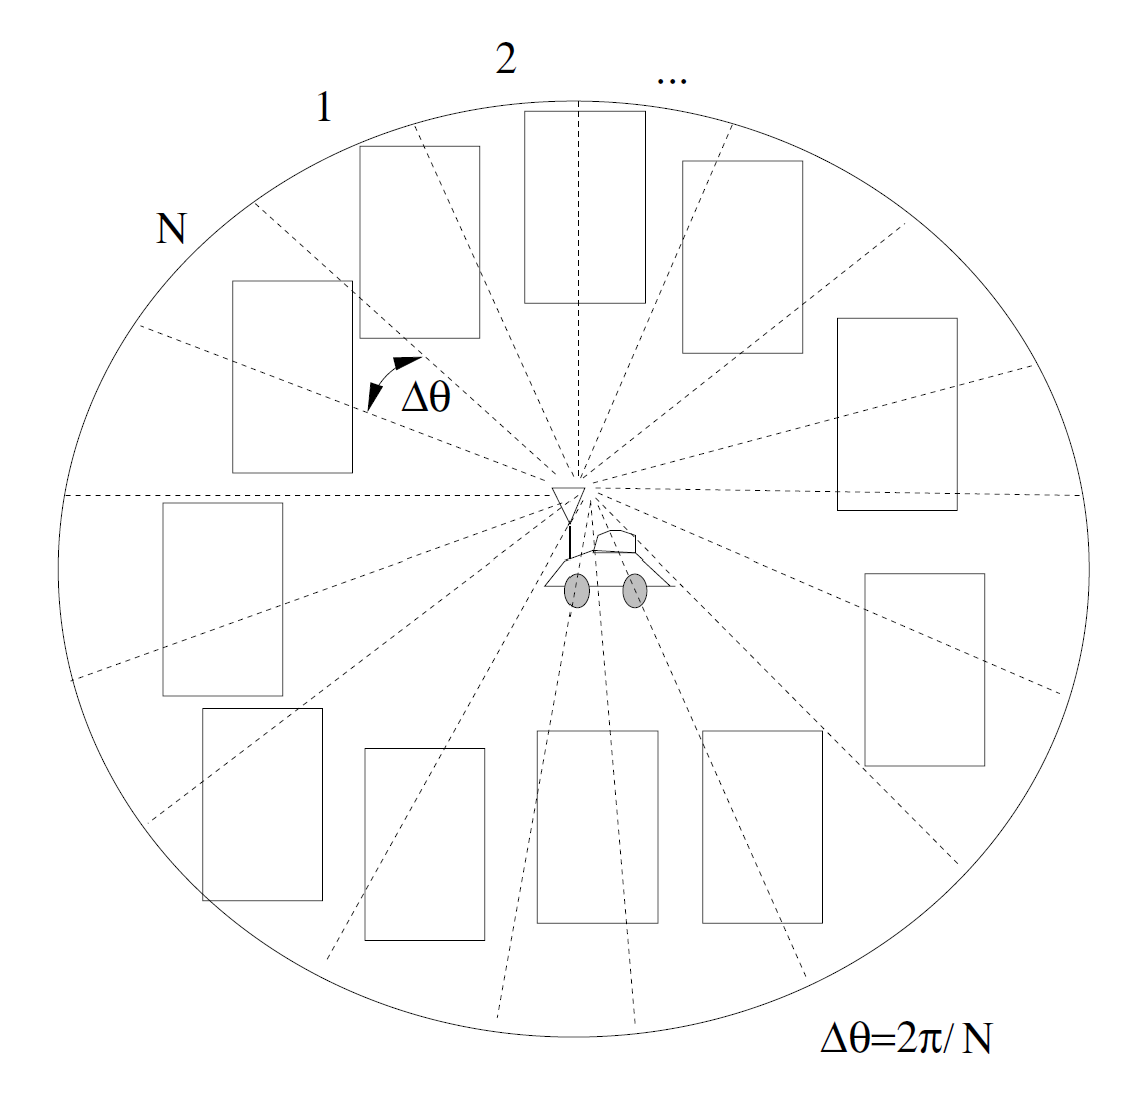
\includegraphics[width=0.6\textwidth]{fig/fig18.png}
	\caption{Simplex kommunikation}
	\label{fig:simplex}
\end{figure}

\noindent Et duplex system er designet til at sende beskeder i begge retninger. Half duplex opstår, når data kan strømme i begge retninger, men kun i én retning ad gangen (Figur \ref{fig:half-duplex}).
\begin{figure}[h]
	\centering
	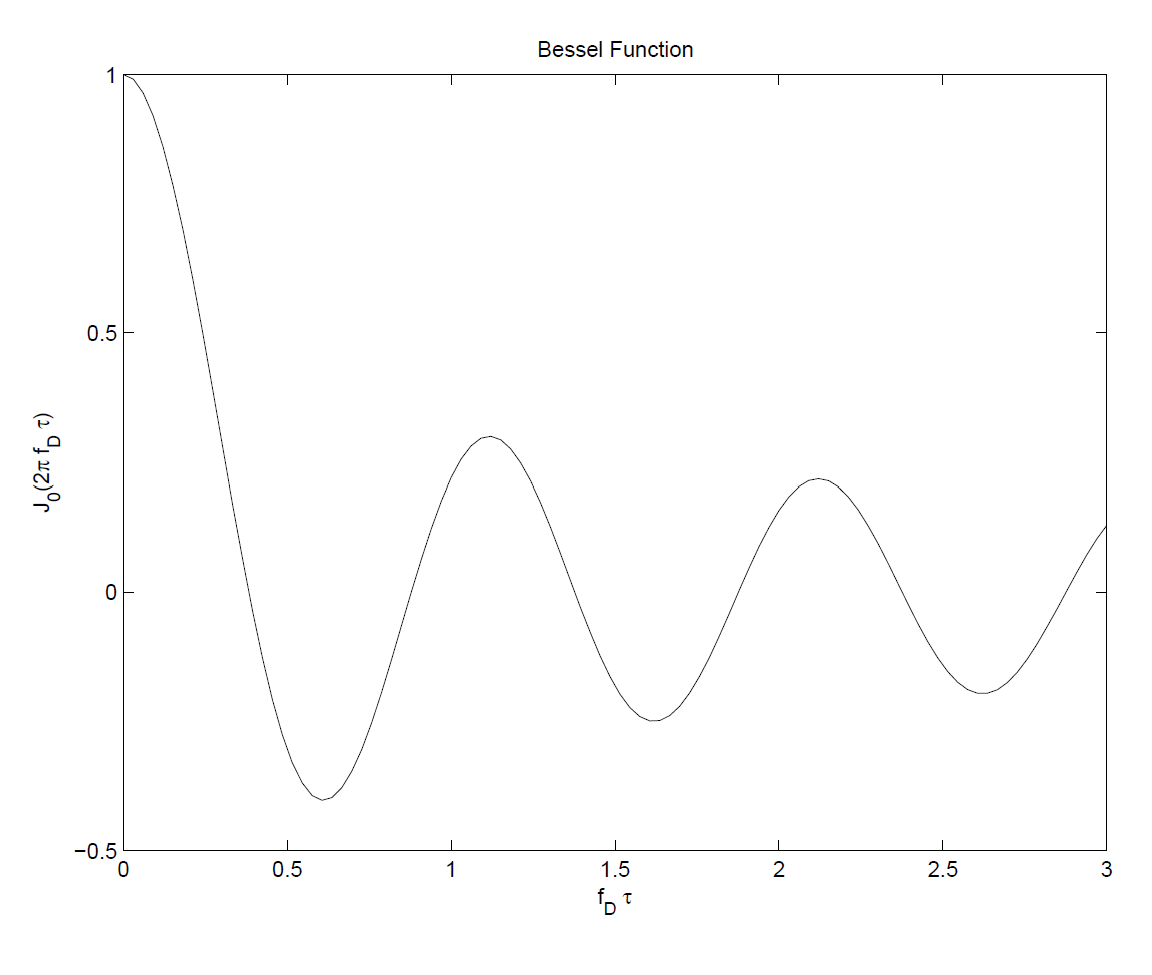
\includegraphics[width=0.6\textwidth]{fig/fig19.png}
	\caption{Half-Duplex kommunikation}
	\label{fig:half-duplex}
\end{figure}

\noindent I et full-duplex system kan data strømme i begge retninger samtidig (Figur \ref{fig:full-duplex}).
\begin{figure}[h]
	\centering
	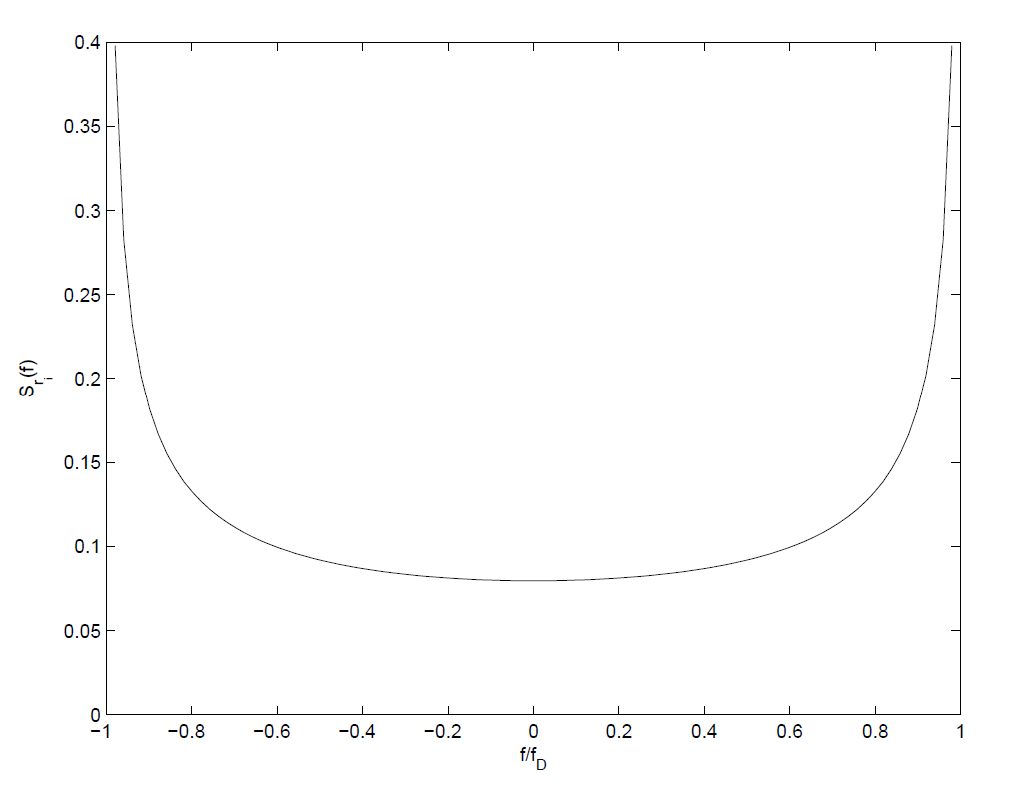
\includegraphics[width=0.6\textwidth]{fig/fig20.png}
	\caption{Full-Duplex kommunikation}
	\label{fig:full-duplex}
\end{figure}

\section{Asynkrone systemer}
Et asynkront system er et, hvor hvert tegn eller byte sendes inden for en ramme. Modtageren begynder ikke at detektere, før den modtager den første bit, kendt som 'startbiten'.
\newline\newline\noindent
\textbf{Startbit:} Startbiten er i den modsatte spændingstilstand i forhold til hvilspændingen og tillader modtageren at synkronisere med senderen for de følgende data i rammen.
\newline\newline\noindent
\textbf{Modtagelse af bits:} Modtageren læser de enkelte bits i rammen, efterhånden som de ankommer, og ser enten logisk 0-spændingen eller logisk 1-spændingen på det rette tidspunkt. 'Clock'-hastigheden i hver ende skal være den samme, så modtageren ser efter hver bit på det tidspunkt, hvor senderen sender den.
\newline\newline\noindent
\textbf{Synkronisering:} Da urene er synkroniseret i starten af hver ramme, kan der tolereres nogen variation ved lavere transmissionshastigheder. Den tilladte variation falder, når dataoverførselshastighederne stiger, og asynkron kommunikation kan have problemer ved høje hastigheder (over 100 kbps).

\section{Meddelelsesformat}
En asynkron ramme kan have følgende format:
\begin{itemize}
	\item \textbf{Startbit:} Signalerer starten af rammen
	\item \textbf{Data:} Normalt 7 eller 8 bits data, men kan være 5 eller 6 bits
	\item \textbf{Paritetsbit:} Valgfri fejldetektionsbit
	\item \textbf{Stopbit(er):} Normalt 1, 1,5 eller 2 bits. En værdi på 1,5 betyder, at niveauet holdes 1,5 gange så længe som en enkelt bit.
\end{itemize}

\begin{figure}[h]
	\centering
	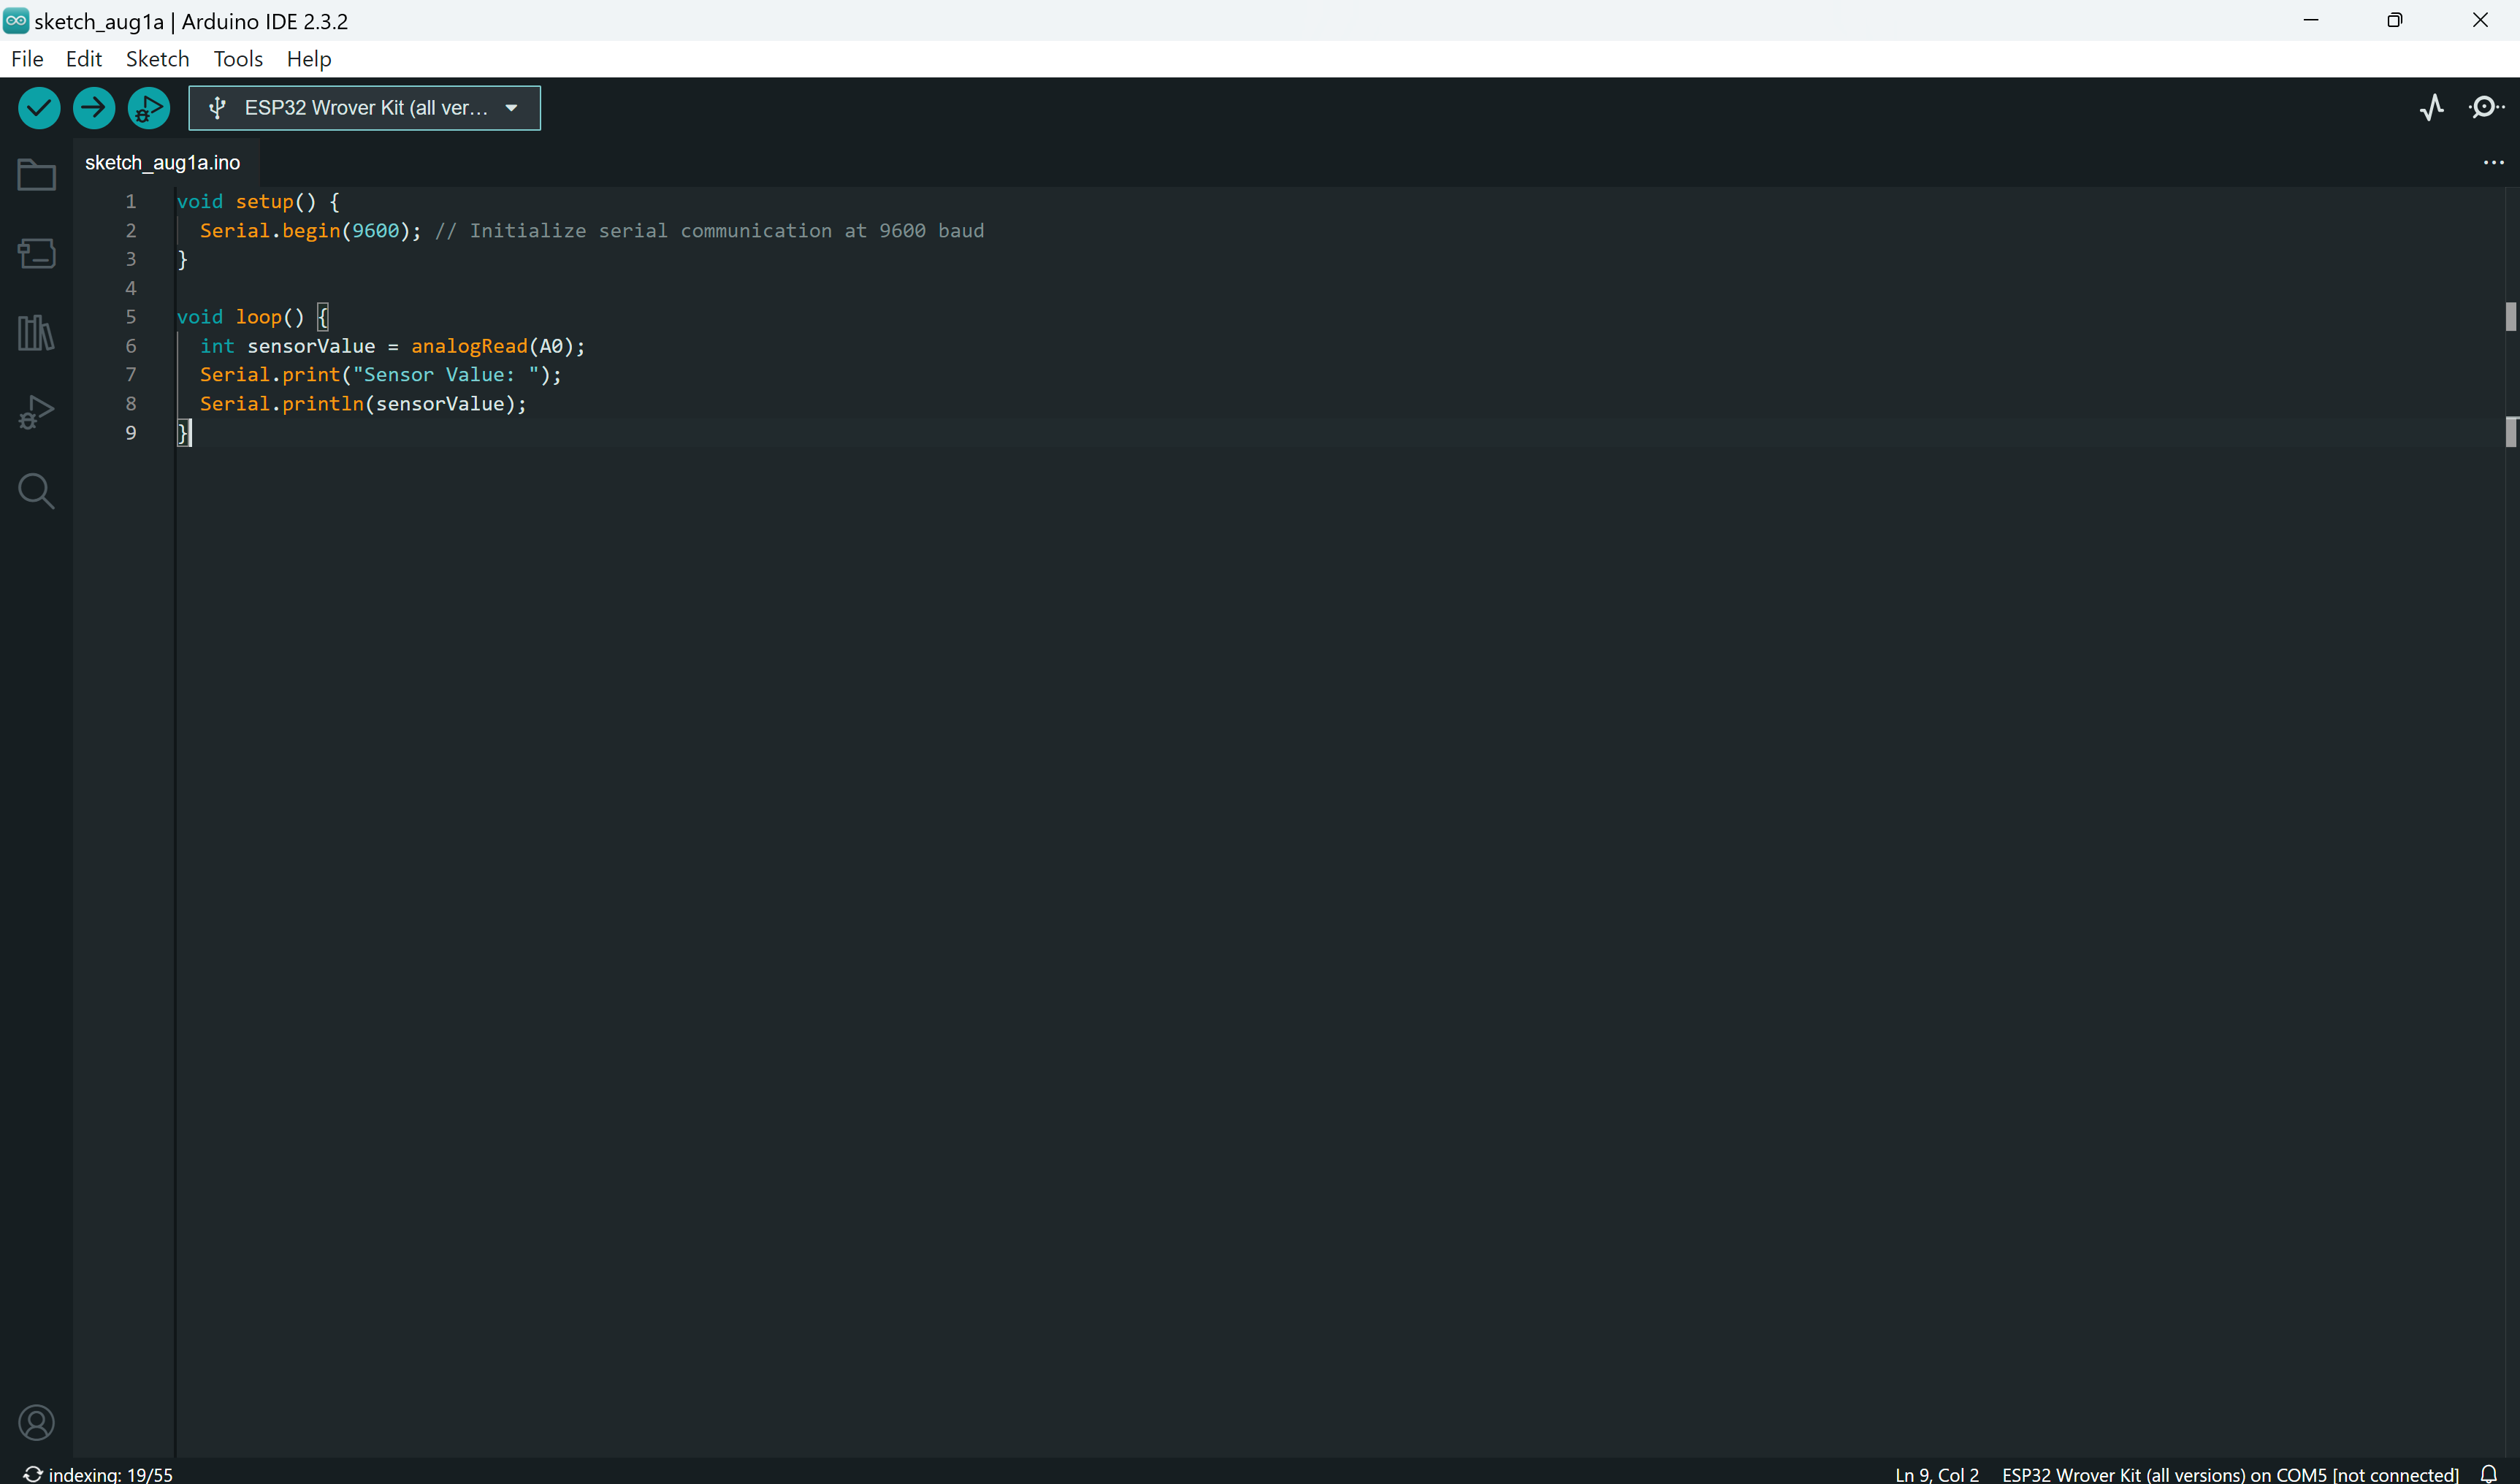
\includegraphics[width=0.8\textwidth]{fig/fig21.png}
	\caption{Asynkront rammeformat}
	\label{fig:asynchronous_frame}
\end{figure}
\noindent Et asynkront rammeformat er vist i Figur \ref{fig:asynchronous_frame}. Senderen og modtageren skal indstilles til præcis den samme konfiguration, så dataene kan udtrækkes korrekt fra rammen. Da hvert tegn har sin egen ramme, er den faktiske dataoverførselshastighed mindre end bithastigheden. For eksempel, med en startbit, syv databits, en paritetsbit og en stopbit, er der ti bits nødvendige for at sende syv bits data. Derfor er transmissionen af nyttige data 70\% af den samlede bithastighed.

\section{Synkrone systemer}
I synkrone systemer synkroniserer modtageren indledningsvis til senderens klokkeimpulser, som er indlejret i de transmitterede datastrømme. Dette gør det muligt for modtageren at opretholde sin synkronisering gennem store beskeder, som typisk kan være op til 4500 bytes (36 000 bits). Dette tillader store rammer at blive transmitteret effektivt ved høje datahastigheder. Det synkrone system pakker mange tegn sammen og sender dem som en kontinuerlig strøm, kaldet en pakke eller en ramme.

\section{Meddelelsesformat}
Et typisk synkront system rammeformat er vist i Figur \ref{fig:synchronous_frame}.
\begin{figure}[h]
	\centering
	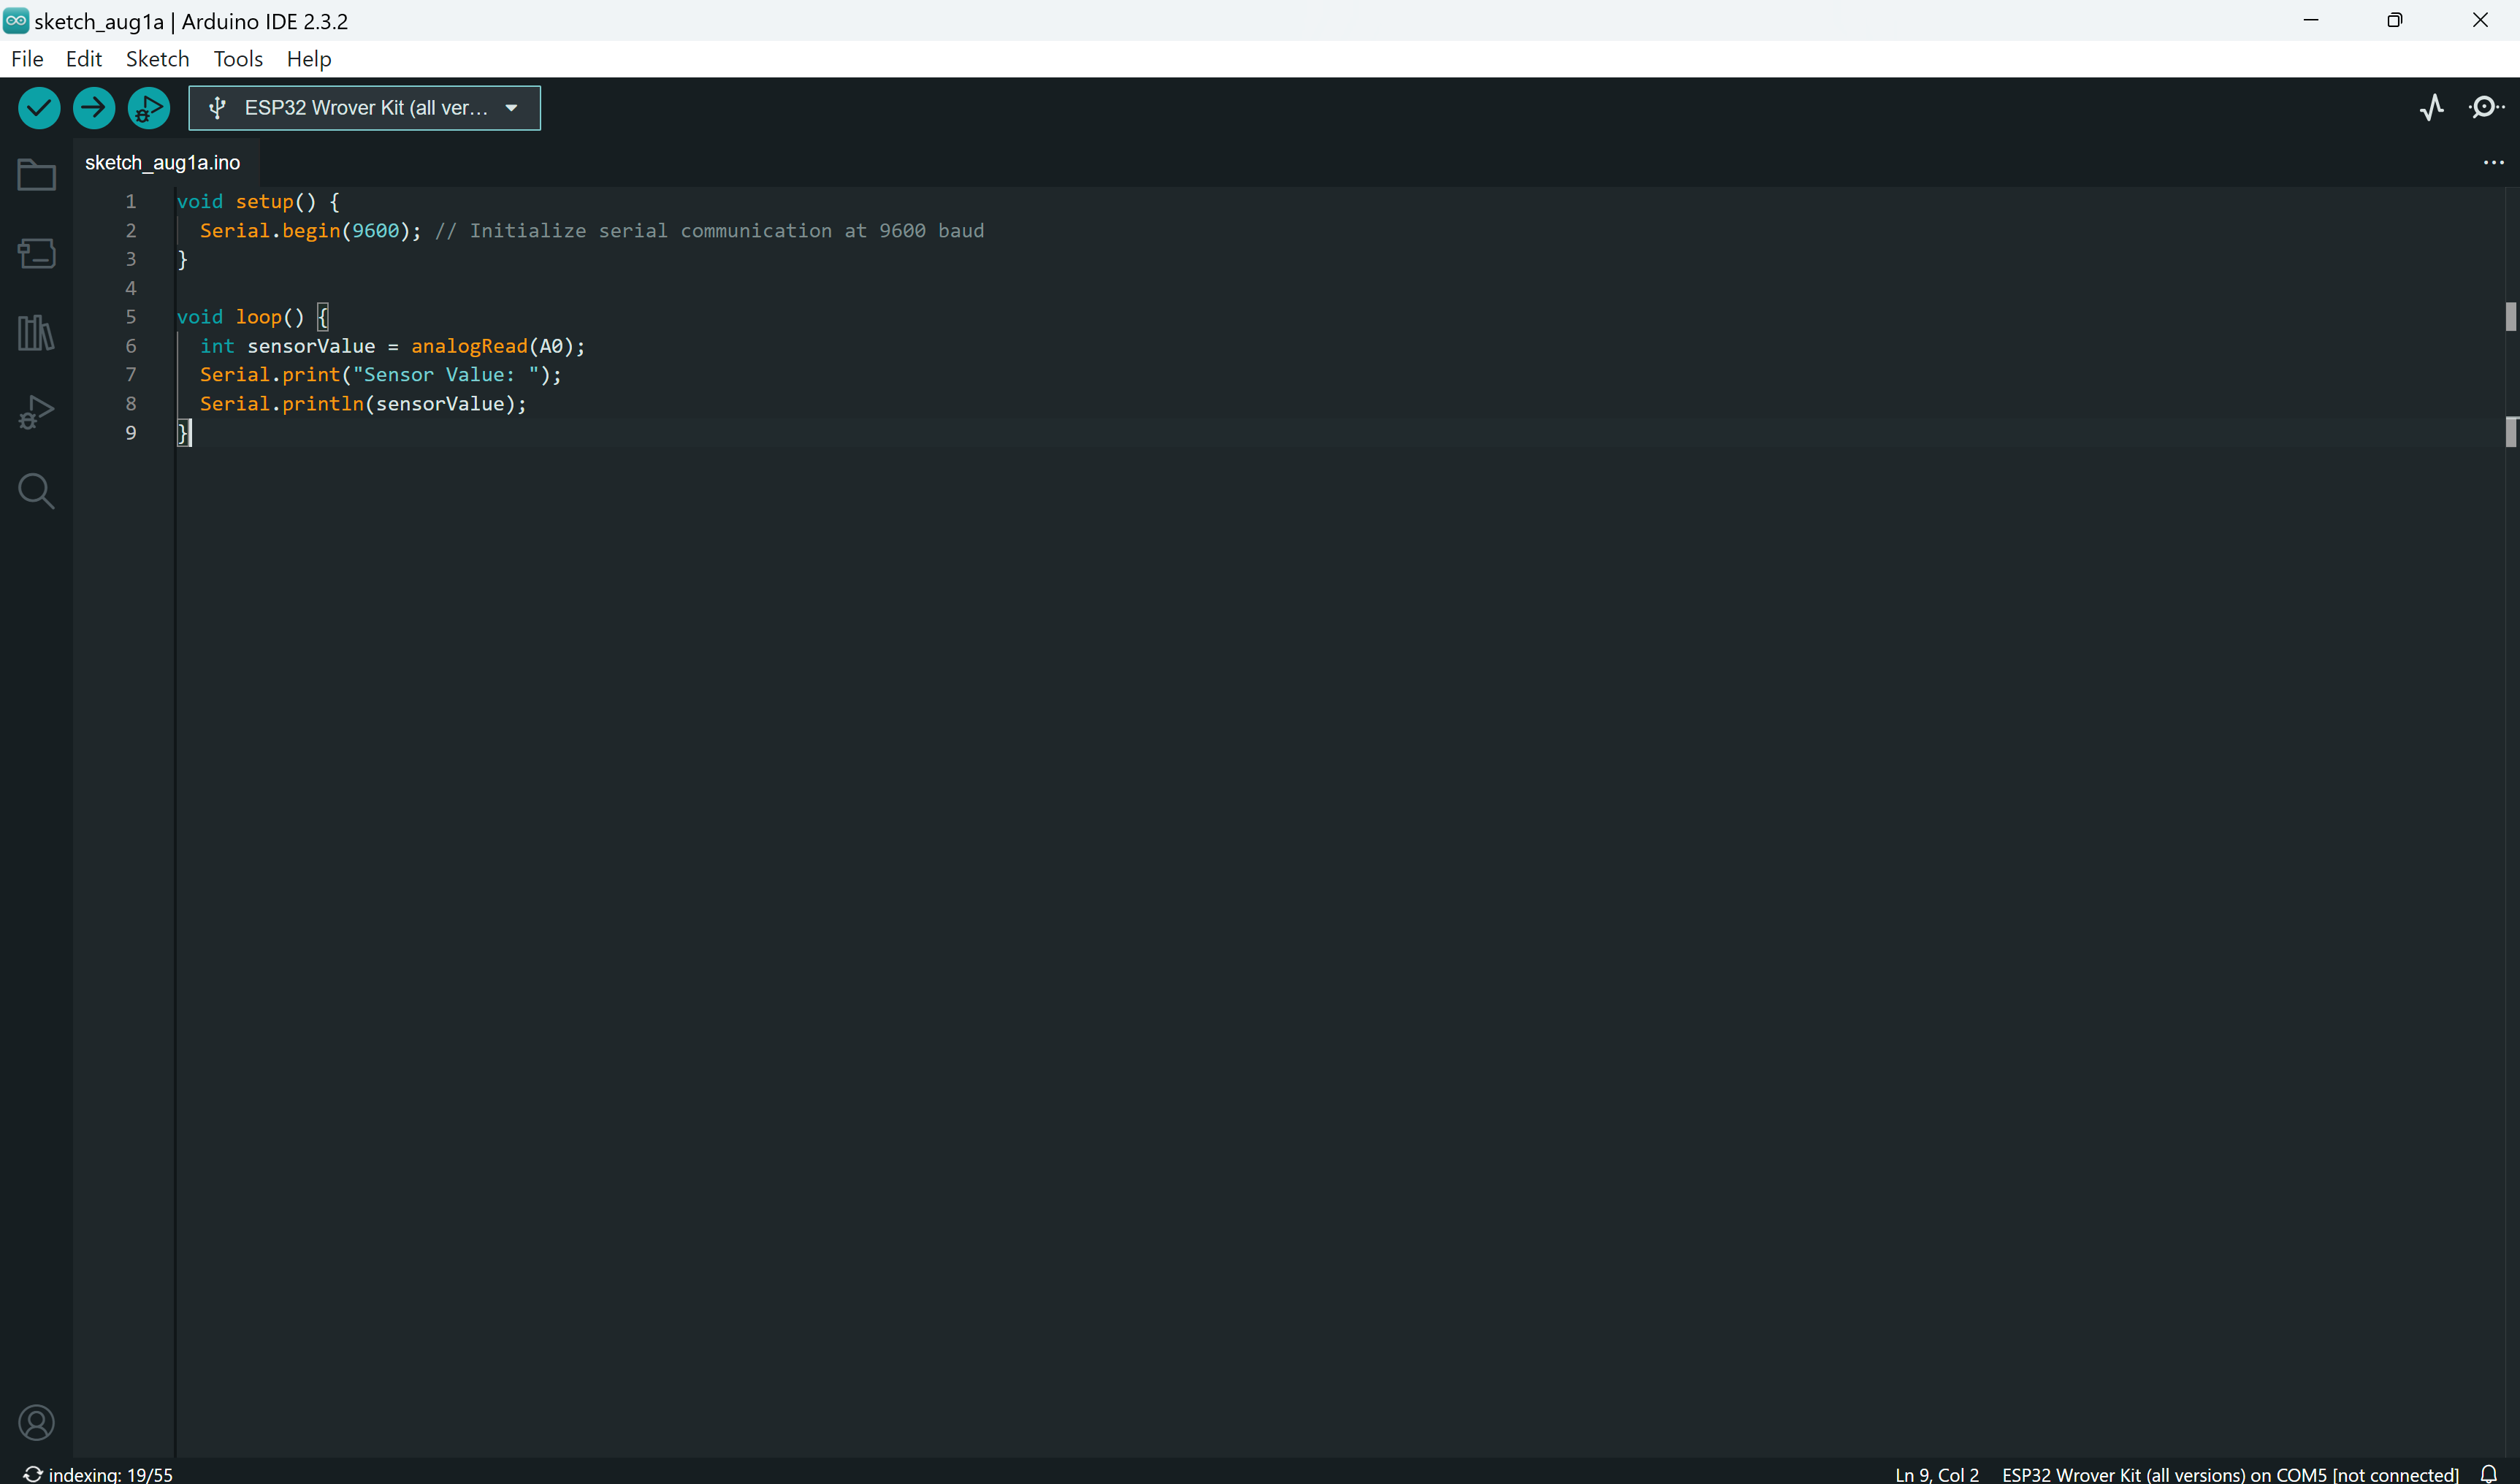
\includegraphics[width=0.8\textwidth]{fig/fig21.png}
	\caption{Typisk synkront system rammeformat}
	\label{fig:synchronous_frame}
\end{figure}

\begin{itemize}
	\item \textbf{Preamble:} Dette omfatter en eller flere bytes, der gør det muligt for modtageren at synkronisere med rammen.
	\item \textbf{SFD:} Start af ramme delimitter signalerer starten af rammen.
	\item \textbf{Destination:} Adressen, som rammen sendes til.
	\item \textbf{Source:} Adressen, som rammen stammer fra.
	\item \textbf{Length:} Antallet af bytes i datafeltet.
	\item \textbf{Data:} Den faktiske besked.
	\item \textbf{FCS:} Frame check sequence er til fejldetektion.
\end{itemize}

\paragraph{Definition og Grundlæggende Koncept}
Seriel kommunikation er en teknik, hvor data overføres én bit ad gangen over en enkelt kommunikationskanal, som typisk er en ledning eller et kabel. Denne form for kommunikation bruges ofte, når data skal sendes over længere afstande, eller hvor det er vigtigt at minimere antallet af ledninger, der er nødvendige for kommunikationen.
\newline\newline\noindent
I modsætning til seriel kommunikation involverer parallel kommunikation overførsel af flere bits samtidigt over flere kanaler eller ledninger. Selvom parallel kommunikation kan opnå højere datahastigheder på korte afstande, kræver den flere ledninger og kan være mere udsat for interferens og synkroniseringsproblemer, især over lange afstande.
\newline\newline\noindent
Den primære fordel ved seriel kommunikation er dens enkelhed og pålidelighed, især i miljøer, hvor der er behov for kommunikation over lange kabler. Det reducerede antal ledninger mindsker risikoen for støj og signalforvrængning, hvilket gør seriel kommunikation ideel til mange industrielle applikationer, hvor robusthed og stabilitet er afgørende.
\newline\newline\noindent
Seriel kommunikation anvender typisk standarder som RS232, RS422 og RS485, der hver især har deres egne specifikationer og anvendelsesområder, afhængigt af kravene til datahastighed, rækkevidde og interferensbeskyttelse.

\chapter{Industriel Seriel Kommunikation og Feltbusprotokoller}
\section{RS232}
RS232 (Recommended Standard 232) er en standard for seriel kommunikation, der er udviklet af Electronic Industries Alliance (EIA). Den bruges primært til at forbinde dataterminaludstyr (DTE) såsom computere til datakommunikationsudstyr (DCE) såsom modemmer. RS232-standardens primære formål er at definere elektriske egenskaber, signalering og timing for serielle dataoverførsler mellem enheder.

\subsection{Fysiske Lag}
RS232 definerer det fysiske lag af kommunikationsforbindelsen, herunder stiktyper, kabler og elektriske signaler. Den mest almindelige stiktype er DB9 (9-pins) eller DB25 (25-pins), selvom andre konfigurationer også findes.
\begin{figure}[h]
	\centering
	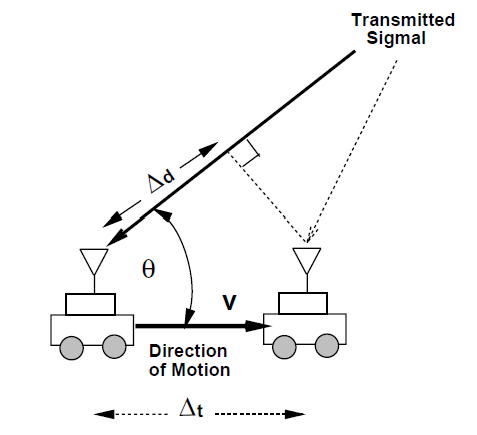
\includegraphics[width=0.5\textwidth]{fig/fig2.png} % Inkluder et billede af RS232-stikket her
	\caption{DB9 stik for RS232}
	\label{fig:rs232_connector}
\end{figure}

\subsection{Elektriske Signaler}
RS232 bruger single-ended signalering, hvilket betyder, at signalet sendes som en spændingsforskel mellem en signalleder og en fælles jordleder. Typiske spændingsniveauer er:

\begin{itemize}
	\item \textbf{Logisk 0 (Marking)}: +3V til +15V
	\item \textbf{Logisk 1 (Spacing)}: -3V til -15V
\end{itemize}
Støjniveauer under ±3V betragtes som udefinerede, hvilket skaber en bufferzone for at minimere signalforstyrrelser.

\subsection{Signalering og Pins}
De vigtigste signaler og deres respektive pins i et DB9-stik er som følger:
\textbf{Pin 1}: DCD (Data Carrier Detect) \\ 
Angiver, at modemet har opdaget en bærer fra fjernmodemet.
\newline
\newline
\textbf{Pin 2}: RXD (Receive Data) \\ 
Bruges til at modtage data fra fjernmodemet.
\newline
\newline
\textbf{Pin 3}: TXD (Transmit Data) \\ 
Bruges til at sende data til fjernmodemet.
\newline
\newline
\textbf{Pin 4}: DTR (Data Terminal Ready) \\ 
Signalerer, at terminalen eller computeren er klar til at kommunikere.
\newline
\newline
\textbf{Pin 5}: GND (Signal Ground) \\ 
Fælles jordforbindelse for alle signaler.
\newline
\newline
\textbf{Pin 6}: DSR (Data Set Ready) \\ 
Indikerer, at modemet er klar til at kommunikere.
\newline
\newline
\textbf{Pin 7}: RTS (Request To Send) \\ 
Bruges til at anmode om tilladelse til at sende data.
\newline
\newline
\textbf{Pin 8}: CTS (Clear To Send) \\ 
Signalerer, at det er klart at modtage data.
\newline
\newline
\textbf{Pin 9}: RI (Ring Indicator) \\ 
Indikerer, at der kommer et indgående opkald.bab
\begin{figure}[!h]
	\centering
	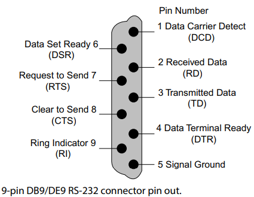
\includegraphics[width=.6\textwidth]{fig/fig3}
	\label{fig:fig3}
\end{figure}

\subsection{Dataoverførsel}
RS232 bruger asynkron dataoverførsel, hvilket betyder, at data sendes i et kontinuerligt strøm af bits uden en fast tidsbase. Dataoverførslen styres af start- og stopbits, som definerer begyndelsen og slutningen af hver dataramme. En typisk dataramme består af:
\begin{itemize}
	\item \textbf{Startbit}: 1 bit (logisk 0)
	\item \textbf{Databits}: 5 til 9 bits (typisk 8 bits)
	\item \textbf{Paritetsbit}: 1 bit (valgfri, bruges til fejlregistrering)
	\item \textbf{Stopbits}: 1, 1.5 eller 2 bits (logisk 1)
\end{itemize}

\subsection{Baudrate}
Baudrate refererer til antallet af signalændringer pr. sekund og bestemmer dataoverførselshastigheden. Typiske baudrater for RS232 er 9600, 19200, 38400, 57600 og 115200 baud. Det er vigtigt, at begge kommunikerende enheder er indstillet til samme baudrate for at sikre korrekt dataoverførsel.

\subsection{Fejlhåndtering}
RS232 anvender enkle fejlhåndteringsmetoder som paritetskontrol, hvor en ekstra bit føjes til hver dataramme for at gøre antallet af 1'er enten lige (even parity) eller ulige (odd parity). Hvis det modtagne antal 1'er ikke matcher den forventede paritet, registreres en fejl.

\subsection{Anvendelser}
RS232 er blevet brugt i en lang række applikationer, herunder:

\begin{itemize}
	\item Forbindelse af computere til modemmer
	\item Industriel automation og kontrolsystemer
	\item Seriel kommunikation med mikrokontrollere og indlejrede systemer
	\item Diagnostisk interface til netværksudstyr
\end{itemize}

\subsection{Fordele og Ulemper}
\begin{itemize}
	\item \textbf{Fordele:}
	\begin{itemize}
		\item Simpel og udbredt standard
		\item Velegnet til korte afstande og lave hastigheder
	\end{itemize}
	\item \textbf{Ulemper:}
	\begin{itemize}
		\item Begrænset dataoverførselshastighed og afstand
		\item Følsom overfor elektrisk støj
		\item Kræver flere ledninger til fuld duplex kommunikation
	\end{itemize}
\end{itemize}
RS232 har været en grundlæggende teknologi i mange år og bruges stadig i dag på trods af fremkomsten af mere avancerede serielle kommunikationsstandarder som USB og RS485.

\section{RS422}
RS422 (Recommended Standard 422) er en standard for seriel dataoverførsel, som er udviklet af Electronic Industries Alliance (EIA). RS422 blev designet til at forbedre de begrænsninger, der findes i RS232, især med hensyn til dataoverførselshastighed og afstand. RS422 anvender differentiel signalering, hvilket gør den mere robust overfor elektrisk støj og muliggør længere kommunikationsafstande.

\subsection{Fysiske Lag}
RS422 definerer det fysiske lag af kommunikationsforbindelsen, inklusive stiktyper, kabler og elektriske signaler. De mest almindelige stiktyper er DB9 (9-pins) og DB25 (25-pins), men andre konfigurationer findes også.
\begin{figure}[h]
	\centering
	
	\caption{DB9 stik for RS422}
	\label{fig:rs422_connector}
\end{figure}

\subsection{Elektriske Signaler}
RS422 bruger differentiel signalering, hvilket betyder, at signalet sendes som en spændingsforskel mellem to ledninger (A og B). Dette reducerer følsomheden overfor elektromagnetisk interferens (EMI). Typiske spændingsniveauer er:

\begin{itemize}
	\item \textbf{Logisk 0 (Marking)}: -2V til -6V (A-B)
	\item \textbf{Logisk 1 (Spacing)}: +2V til +6V (A-B)
\end{itemize}

\subsection{Signalering og Pins}
De vigtigste signaler og deres respektive pins i et DB9-stik er som følger:

\begin{itemize}
	\item \textbf{Pin 1}: GND (Signal Ground)
	\item \textbf{Pin 2}: TXD+ (Transmit Data Positive)
	\item \textbf{Pin 3}: TXD- (Transmit Data Negative)
	\item \textbf{Pin 4}: RXD+ (Receive Data Positive)
	\item \textbf{Pin 5}: RXD- (Receive Data Negative)
	\item \textbf{Pin 6-9}: Ikke brugt eller valgfri for kontrolsignaler
\end{itemize}

\subsection{Dataoverførsel}
RS422 understøtter asynkron og synkron dataoverførsel. Asynkron overførsel bruger start- og stopbits til at definere begyndelsen og slutningen af en dataramme, mens synkron overførsel bruger en klokkesignal til at synkronisere dataoverførslen.

\subsection{Baudrate og Afstand}
RS422 kan understøtte dataoverførselshastigheder op til 10 Mbps over korte afstande (op til 12 meter). Over længere afstande (op til 1200 meter) kan hastigheder op til 100 kbps opnås. Det er vigtigt at matche baudraten på begge kommunikerende enheder for at sikre korrekt dataoverførsel.

\subsection{Fejlhåndtering}
RS422's differentielle signalering reducerer fejl forårsaget af elektrisk støj. Desuden kan paritetskontrol og andre fejldetekteringsmetoder anvendes for at sikre dataintegritet.

\subsection{Anvendelser}
RS422 anvendes ofte i industrielle og kommercielle applikationer, herunder:
\begin{itemize}
	\item Industriel automation og kontrolsystemer
	\item Seriel kommunikation mellem computere og periferiudstyr
	\item Netværksforbindelser over lange afstande
	\item Kommunikationslinjer i høj EMI-miljøer
\end{itemize}

\subsection{Fordele og Ulemper}
\begin{itemize}
	\item \textbf{Fordele:}
	\begin{itemize}
		\item Højere dataoverførselshastigheder og længere rækkevidde sammenlignet med RS232.
		\item Robust overfor elektrisk støj på grund af differentiel signalering.
		\item Mulighed for at forbinde flere modtagere (op til 10) på samme sender.
	\end{itemize}
	\item \textbf{Ulemper:}
	\begin{itemize}
		\item Mere kompleks end RS232 med hensyn til kabelføring og stik.
		\item Kræver specielle drivere og modtagere til differentiel signalering.
	\end{itemize}
\end{itemize}
RS422 er en kraftfuld standard for seriel kommunikation, der tilbyder højere hastigheder og længere afstande end RS232, hvilket gør den velegnet til krævende industrielle applikationer.

\section{RS485}
RS485 (Recommended Standard 485) er en standard for seriel dataoverførsel, udviklet af Electronic Industries Alliance (EIA). RS485 er designet til at muliggøre pålidelig kommunikation over lange afstande og i støjfyldte miljøer. Den anvender differentiel signalering, som gør den robust overfor elektromagnetisk interferens (EMI) og tillader multi-drop netværk, hvor flere enheder kan kommunikere over samme bus.

\subsection{Fysiske Lag}
RS485 definerer det fysiske lag af kommunikationsforbindelsen, herunder stiktyper, kabler og elektriske signaler. De mest almindelige stiktyper er terminalblokke og DB9-stik.
\begin{figure}[h]
	\centering
	%\includegraphics[width=0.5\textwidth]{rs485_connector.png} % Inkluder et billede af RS485-stikket her
	\caption{Terminalblok stik for RS485}
	\label{fig:rs485_connector}
\end{figure}

\subsection{Elektriske Signaler}
RS485 bruger differentiel signalering, hvilket betyder, at signalet sendes som en spændingsforskel mellem to ledninger (A og B). Dette reducerer følsomheden overfor EMI. Typiske spændingsniveauer er:
\begin{itemize}
	\item \textbf{Logisk 0 (Marking)}: -1.5V til -5V (A-B)
	\item \textbf{Logisk 1 (Spacing)}: +1.5V til +5V (A-B)
\end{itemize}

\subsection{Signalering og Pins}
De vigtigste signaler og deres respektive pins i et typisk terminalblok-stik er som følger:
\begin{itemize}
	\item \textbf{Pin 1}: A (Data Line Positive)
	\item \textbf{Pin 2}: B (Data Line Negative)
	\item \textbf{Pin 3}: GND (Signal Ground)
	\item \textbf{Pin 4-5}: Valgfri for terminering eller skærmning
\end{itemize}

\subsection{Dataoverførsel}
RS485 understøtter både asynkron og synkron dataoverførsel. Asynkron overførsel bruger start- og stopbits til at definere begyndelsen og slutningen af en dataramme, mens synkron overførsel bruger et klokkesignal til at synkronisere dataoverførslen. RS485 tillader også multi-drop netværk, hvilket betyder, at op til 32 enheder kan tilsluttes på samme bus.

\subsection{Baudrate og Afstand}
RS485 kan understøtte dataoverførselshastigheder op til 10 Mbps over korte afstande (op til 15 meter). Over længere afstande (op til 1200 meter) kan hastigheder op til 100 kbps opnås. Det er vigtigt at matche baudraten på alle kommunikerende enheder for at sikre korrekt dataoverførsel.

\subsection{Fejlhåndtering}
RS485's differentielle signalering reducerer fejl forårsaget af elektrisk støj. Desuden kan paritetskontrol og andre fejldetekteringsmetoder anvendes for at sikre dataintegritet. RS485-netværk kan også bruge terminering modstande for at minimere refleksioner på kablet, hvilket forbedrer signalintegriteten.

\subsection{Anvendelser}
RS485 anvendes ofte i industrielle og kommercielle applikationer, herunder:
\begin{itemize}
	\item Industriel automation og kontrolsystemer
	\item Seriel kommunikation mellem computere og periferiudstyr
	\item Netværksforbindelser over lange afstande
	\item Kommunikationslinjer i høj EMI-miljøer
	\item Bygningsautomation (f.eks. HVAC-systemer, belysningskontrol)
\end{itemize}

\subsection{Fordele og Ulemper}
\begin{itemize}
	\item \textbf{Fordele:}
	\begin{itemize}
		\item Højere dataoverførselshastigheder og længere rækkevidde sammenlignet med RS232.
		\item Robust overfor elektrisk støj på grund af differentiel signalering.
		\item Mulighed for at forbinde op til 32 enheder på samme bus (kan udvides med repeaters).
	\end{itemize}
	\item \textbf{Ulemper:}
	\begin{itemize}
		\item Mere kompleks end RS232 med hensyn til kabelføring og stik.
		\item Kræver specielle drivere og modtagere til differentiel signalering.
		\item Kan være komplekst at konfigurere og fejlfinde i store netværk.
	\end{itemize}
\end{itemize}
RS485 er en kraftfuld standard for seriel kommunikation, der tilbyder højere hastigheder, længere afstande og multi-drop kapaciteter, hvilket gør den velegnet til krævende industrielle applikationer.

\section{DeviceNet}
DeviceNet er en industriel netværksprotokol, der bruges til at forbinde industrielle enheder såsom sensorer, aktuatorer og controllere. Det er en del af CIP (Common Industrial Protocol) og bruges ofte i automatiseringssystemer til at sikre pålidelig og effektiv kommunikation mellem enheder.

\subsection{Introduktion}
DeviceNet er designet til at være en fleksibel og skalerbar løsning til industriel kommunikation. Det giver mulighed for at tilføje og fjerne enheder uden at forstyrre det overordnede system, hvilket gør det ideelt til brug i dynamiske miljøer, hvor kravene til netværket kan ændre sig over tid.
\begin{figure}[!h]
	\centering
	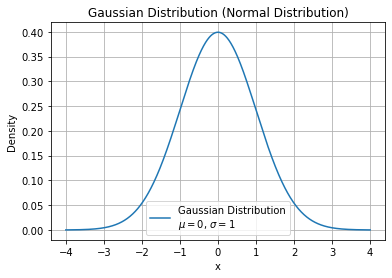
\includegraphics[width=\linewidth]{fig/fig13}
\end{figure}

\subsection{Fysisk Lag}
\subsection*{Topologi}
DeviceNet bruger en bus-topologi, hvor alle enheder er forbundet til en fælles kommunikationsbus. Dette layout er både simpelt og økonomisk, da det kræver minimal kabling og giver nem adgang til alle enheder på netværket. Det understøtter også stjerne- og trunk-line topologier, hvilket giver fleksibilitet i netværksdesign.

\subsection{Stikforbindelser}
\subsection*{Pluggbare (utætte) stik}
Disse stik er nemme at tilslutte og afbryde, hvilket gør dem ideelle til brug i miljøer, hvor hurtig installation og vedligeholdelse er nødvendig. De er dog ikke tætte og bør derfor ikke bruges i miljøer, hvor de kan udsættes for væsker eller støv.

\subsection*{Fastforbundne (utætte) stik}
Ligesom de pluggable stik er disse stik ikke tætte, men de giver en mere permanent forbindelse. De bruges ofte i mere stabile miljøer, hvor der ikke er behov for hyppig til- og frakobling.

\subsection*{Mini (tætte) stik}
Disse stik er designet til at være tætte og beskytte mod indtrængen af væsker og støv. De er ideelle til brug i barske industrielle miljøer.

\subsection*{Mikro (tætte) stik}
Mikrostik er mindre end mini-stik, men tilbyder samme niveau af tæthed. De bruges ofte i applikationer, hvor pladsen er begrænset.

\subsection{Kabelbudgetter}
Kabelbudgetter i DeviceNet bestemmer den maksimale længde og type af kabel, der kan bruges, uden at det påvirker netværkets ydeevne. Dette inkluderer overvejelser om signalstyrke, spændingsfald og dataoverførselshastigheder.

\subsection{Enhedstaps}
\subsection*{Tætte taps}
Tætte taps giver en sikker forbindelse, der beskytter mod indtrængen af væsker og støv. De bruges i miljøer, hvor pålidelighed og beskyttelse er afgørende.

\subsection*{IDC taps}
IDC (Insulation Displacement Connector) taps er nemme at installere og kræver ikke, at kablets isolering fjernes. Dette gør installationen hurtigere og reducerer risikoen for skader på kablet.

\subsection*{Åbne taps}
Åbne taps er ikke beskyttede mod miljøpåvirkninger og bør kun bruges i kontrollerede indendørs miljøer.

\subsection*{Multiport åbne taps}
Disse taps giver mulighed for tilslutning af flere enheder på samme punkt, hvilket kan reducere kablingsomkostningerne og forenkle installationen.

\subsection*{Strømtaps}
Strømtaps giver en dedikeret forbindelse til strømforsyning af enheder på netværket, hvilket kan være nødvendigt i applikationer med høje strømkrav.

\subsection{Kabler}
\subsection*{Tykt kabel}
Tykt kabel bruges i DeviceNet-applikationer, hvor lange kabellængder eller høje strømkrav er nødvendige. Det giver lavere modstand og bedre signalintegritet over lange afstande.

\subsection*{Tyndt kabel}
Tyndt kabel bruges i applikationer, hvor pladsen er begrænset, og kabellængderne er korte. Det er lettere at håndtere og installere i trange rum.

\subsection*{Fladt kabel}
Fladt kabel bruges i applikationer, hvor kablet skal lægges under gulve eller tæpper. Det er nemt at skjule og giver en pænere installation.

\subsection{Netværksstrøm}
\subsection*{Generel tilgang}
Netværksstrøm i DeviceNet sikrer, at alle enheder på netværket får tilstrækkelig strøm til at fungere korrekt. Dette inkluderer overvejelser om strømforsyningens kapacitet og distribution.

\subsection*{Enkel forsyning – ende tilsluttet}
Denne tilgang til netværksstrøm bruger en enkelt strømforsyning, der er tilsluttet i enden af netværket. Dette er en simpel og økonomisk løsning, men kan være mindre pålidelig i store netværk.

\subsection*{Enkel forsyning – midter tilsluttet}
Denne tilgang placerer strømforsyningen i midten af netværket, hvilket giver en mere jævn fordeling af strømmen og kan forbedre pålideligheden i større netværk.

\subsection*{Forslag til undgåelse af fejl og strømforsyningsmuligheder}
For at undgå fejl i netværksstrømmen skal der tages højde for faktorer som korrekt dimensionering af strømforsyningen, brug af redundante strømforsyninger og regelmæssig vedligeholdelse.

\subsection{Systemjord}
Systemjord sikrer, at alle enheder på netværket har en fælles jordforbindelse, hvilket er afgørende for at undgå jordsløjfer og signalstøj.

\subsection{Signalering}
DeviceNet bruger signaleringsteknikker til at kommunikere data mellem enheder. Dette inkluderer brugen af specifikke spændingsniveauer og tidsrammer for at sikre pålidelig dataoverførsel.

\subsection{Data Link Lag}	
\subsection*{Rammeformat}
Rammeformatet i DeviceNet definerer strukturen af de data, der overføres mellem enheder. Dette inkluderer felter som start- og stopbits, adresseinformation og fejlkontrol.

\subsection*{Mediumadgang}
Mediumadgang kontrollerer, hvordan enheder får adgang til kommunikationsmediet. DeviceNet bruger en deterministisk tilgang, hvor hver enhed tildeles et bestemt tidspunkt til at sende data.

\subsection*{Fragmentering}
Fragmentering bruges til at opdele store datarammer i mindre dele, der kan overføres effektivt over netværket. Disse fragmenter samles igen ved modtageren for at gendanne den oprindelige data.

\subsection{Applikationslaget}
Applikationslaget i DeviceNet definerer de protokoller og services, der bruges til at udføre specifikke funktioner, såsom læsning og skrivning af data, alarmhåndtering og diagnostik.

\subsection{Fejlfinding}
\subsection*{Introduktion}
Fejlfinding i DeviceNet involverer identifikation og løsning af problemer, der kan påvirke netværkets ydeevne og pålidelighed.

\subsection*{Værktøjer til fejlfinding}
Værktøjer som netværksscannere, multimetre og protokolanalysatorer kan bruges til at diagnosticere problemer i DeviceNet-netværk.

\subsection*{Fejlfindingsprocedurer}
Fejlfindingsprocedurer inkluderer systematisk kontrol af kabler, stik, strømforsyninger og netværkskonfigurationer for at identificere og løse problemer.
\clearpage
\subsection{Opsummering}
DeviceNet er en robust og fleksibel netværksprotokol, der er designet til at opfylde kravene i moderne industrielle automatiseringssystemer. Ved at forstå de forskellige aspekter af DeviceNet, fra fysisk lag til applikationslag og fejlfinding, kan teknikere og ingeniører sikre, at deres netværk fungerer optimalt og pålideligt.
\begin{figure}[!h]
	\centering
	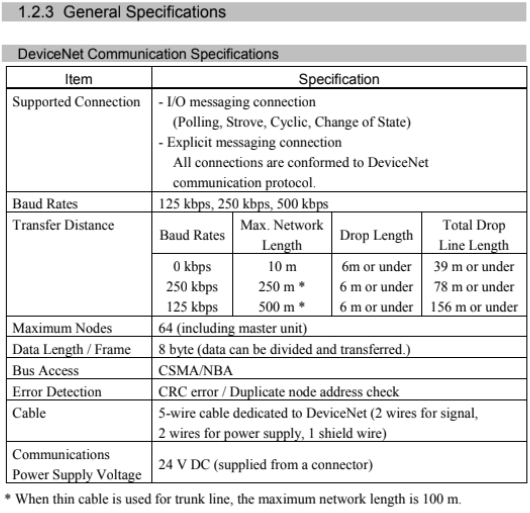
\includegraphics[width=.8\linewidth]{fig/fig14}
\end{figure}
\clearpage
\section{ProfiBus PA/DP/FMS Overview}
ProfiBus (Process Field Bus) er en standardiseret industrielt kommunikationsprotokol, der bruges til at forbinde automatiseringsenheder som sensorer, aktuatorer og controllere. Det er en af de mest udbredte feltbusstandarder i verden og understøtter både procesautomatisering (PA), decentraliseret periferikommunikation (DP) og feltbussystemer (FMS).

\subsection{Introduktion}
ProfiBus er udviklet til at muliggøre hurtig og pålidelig kommunikation mellem industrielle enheder. Det er en alsidig protokol, der kan bruges i en bred vifte af applikationer, herunder fabriksautomatisering, proceskontrol og bygningsautomatisering.

\subsection{ProfiBus Protocol Stack}
ProfiBus-protokollen er opdelt i flere lag, som hver især håndterer forskellige aspekter af kommunikationen. Denne lagdelte arkitektur gør det muligt at isolere og håndtere forskellige funktioner effektivt.

\subsection*{Fysisk Lag (Layer 1)}
Det fysiske lag i ProfiBus definerer de elektriske og mekaniske egenskaber ved netværksforbindelserne. Dette inkluderer specifikationer for kabler, stik og elektriske signaler, der bruges til at overføre data mellem enheder.

\subsection*{Datalink Lag (Layer 2)}
Datalink-laget håndterer pålidelig overførsel af data mellem enheder på netværket. Dette inkluderer fejlregistrering og korrektion, adressering af enheder og styring af datarammer.

\subsection*{Applikationslag}
Applikationslaget definerer de protokoller og tjenester, der bruges til at udføre specifikke funktioner som læsning og skrivning af data, alarmhåndtering og diagnostik. Dette lag sikrer, at applikationer kan kommunikere effektivt over netværket.

\subsection*{Fieldbus Message Specification (FMS)}
FMS specificerer de meddelelser, der bruges til at kommunikere mellem enheder på feltbusnetværket. Dette inkluderer standarder for meddelelsesformat og kommunikationsprotokoller.

\subsection*{Lower Layer Interface (LLI)}
LLI fungerer som en grænseflade mellem de lavere lag (fysisk og datalink) og de højere lag (applikation og FMS). Det sikrer, at data kan overføres effektivt mellem disse lag.

\subsection*{Fieldbus Management Layer (FMA 7)}
FMA 7 håndterer styring og konfiguration af feltbusnetværket. Dette inkluderer opgaver som netværksinitialisering, konfigurationsstyring og diagnosticering af netværksfejl.

\subsection{ProfiBus Kommunikation Model}
ProfiBus kommunikationsmodellen beskriver, hvordan data overføres mellem enheder på netværket. Dette inkluderer beskrivelser af kommunikationscyklusser, dataoverførselshastigheder og synkroniseringsmetoder.

\subsection{Forhold mellem Applikationsproces og Kommunikation}
Dette afsnit beskriver, hvordan applikationsprocesser interagerer med kommunikationsprotokollen for at sikre effektiv dataoverførsel. Det forklarer, hvordan data fra applikationslaget omsættes til meddelelser, der kan sendes over netværket.

\subsection{Kommunikationsobjekter}
Kommunikationsobjekter i ProfiBus refererer til de enheder, data og tjenester, der kan adresseres og styres over netværket. Dette inkluderer beskrivelser af de forskellige typer af kommunikationsobjekter og deres funktioner.

\subsection{Ydeevne}
Dette afsnit diskuterer ydeevnen af ProfiBus-netværket, herunder dataoverførselshastigheder, responstider og netværkskapacitet. Det giver også retningslinjer for optimering af netværksydeevne.

\subsection{Systemoperation}
\subsection*{Konfiguration}
ProfiBus-netværket kræver korrekt konfiguration for at fungere optimalt. Dette afsnit beskriver de trin, der er nødvendige for at konfigurere enheder, tildele adresser og indstille netværksparametre.

\subsection*{Dataoverførsel mellem DPM1 og DP-slaver}
Dette afsnit beskriver processen for dataoverførsel mellem masterenheden (DPM1) og slaveenhederne (DP-slaver). Det forklarer, hvordan data pakkes, adresseres og sendes over netværket.

\subsection*{Synkronisering og Frysemodi}
Synkronisering og frysemodi bruges til at koordinere dataoverførsel mellem enheder og sikre, at dataene overføres på det rigtige tidspunkt. Dette afsnit beskriver, hvordan disse funktioner implementeres og bruges.

\subsection*{Sikkerhed og Beskyttelse af Stationer}
Sikkerhed og beskyttelse er afgørende for at sikre, at netværket fungerer pålideligt og uden forstyrrelser. Dette afsnit beskriver de mekanismer, der bruges til at beskytte netværket mod fejl og angreb.

\subsection*{Blandet Drift af FMS- og DP-stationer}
Dette afsnit beskriver, hvordan FMS- og DP-stationer kan fungere samtidigt på samme netværk. Det forklarer, hvordan kompatibilitet og interoperabilitet sikres mellem forskellige typer enheder.

\subsection{Fejlfinding}
\subsection*{Introduktion}
Fejlfinding er en vigtig del af vedligeholdelsen af ProfiBus-netværket. Dette afsnit introducerer de grundlæggende principper for fejlfinding og diagnosticering af netværksproblemer.

\subsection*{Fejlfinding Værktøjer}
Der findes forskellige værktøjer, der kan bruges til at diagnosticere og løse problemer i ProfiBus-netværket. Dette afsnit beskriver nogle af de mest almindelige værktøjer og deres anvendelser.

\subsection*{Tips}
Dette afsnit giver praktiske tips til fejlfinding og vedligeholdelse af ProfiBus-netværket. Det inkluderer anbefalinger til forebyggelse af almindelige problemer og optimering af netværksydelsen.

\subsection{Opsummering}
ProfiBus er en alsidig og pålidelig feltbusprotokol, der er designet til at opfylde behovene i moderne industrielle automatiseringssystemer. Ved at forstå de forskellige aspekter af ProfiBus, fra protokolstack til fejlfinding, kan teknikere og ingeniører sikre, at deres netværk fungerer effektivt og pålideligt.
\begin{figure}[!h]
	\centering
	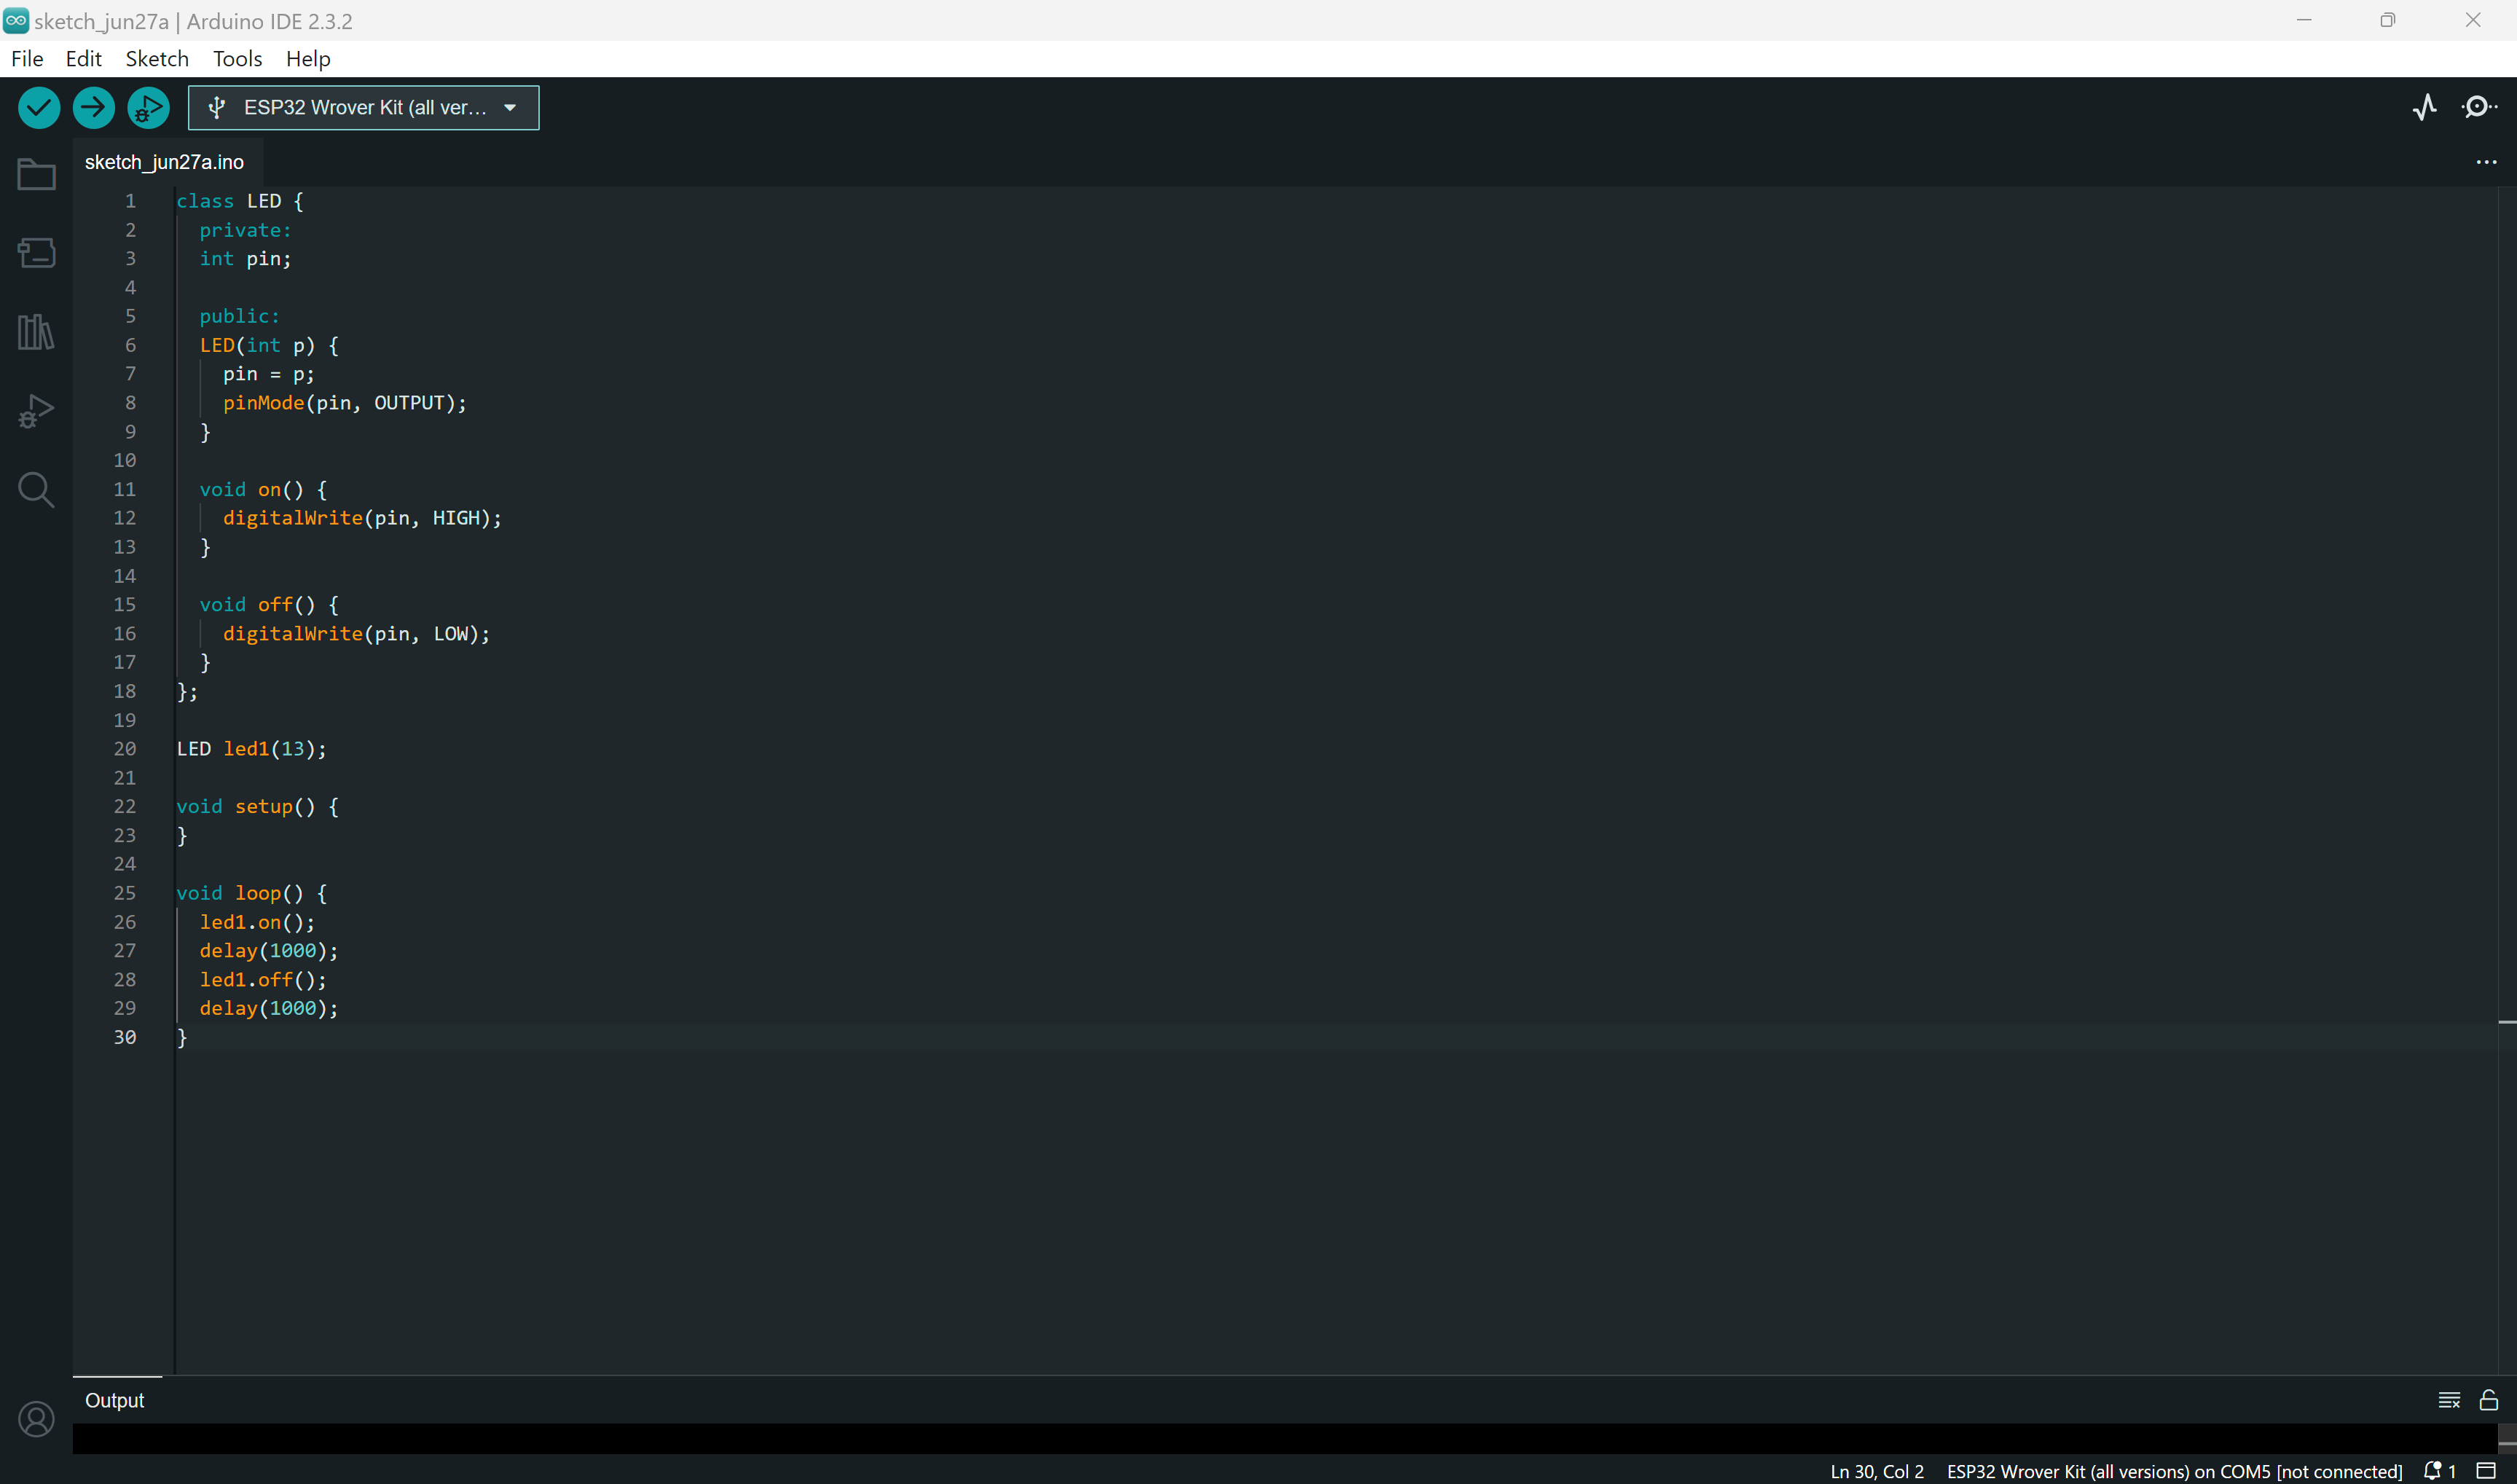
\includegraphics[width=\linewidth]{fig/fig15}
\end{figure}

	% Ethernet-baseret Kommunikation
	\part{Ethernet-baseret Kommunikation}
\chapter{Industriel netværksprotokoller og standarder}	

\section{Modbus}
Modbus er en netværksprotokol med varianter for både seriel og TCP/IP-baseret kommunikation.

\paragraph{Modbus RTU:}
Modbus RTU (Remote Terminal Unit) er en seriel kommunikationsprotokol, der ofte bruges over RS-485-standarden. Den definerer, hvordan data pakkes i enheder kaldet frames og overføres mellem master- og slave-enheder.
\newline\newline 
\noindent\textbf{Protokol:} Modbus RTU beskriver, hvordan data formateres og adresseres inden for en ramme. Den definerer også mekanismer til fejldetektion og fejlkorrektion.
\newline\newline
\noindent\textbf{Elektrisk Standard:} Modbus RTU bruger elektriske standarder som RS-232, RS-422, og mest almindeligt, RS-485 for den fysiske transmission af data. RS-485 muliggør længere kabelafstande og understøtter multi-drop forbindelser.

\paragraph{Modbus TCP:}
Modbus TCP (Transmission Control Protocol) er en version af Modbus-protokollen, der kører over TCP/IP-netværk.
\newline\newline
\noindent\textbf{Protokol:} Modbus TCP definerer, hvordan Modbus-data pakkes inden for TCP/IP-rammer. Det muliggør kommunikation over Ethernet og bruger IP-adresser til at identificere enheder på netværket.
\newline\newline
\noindent\textbf{Elektrisk Standard:} Selvom Modbus TCP primært er en protokol, afhænger den af Ethernet's elektriske standarder for fysiske forbindelser. Dette inkluderer brug af Ethernet-kabler og standard netværksudstyr som switches og routers.

\subsection{Sammenfatning}
Både Profinet og Modbus (RTU og TCP) er primært protokoller, men de har også elektriske specifikationer og krav til det fysiske lag:
\begin{itemize}
	\item \textbf{Profinet:} En industriel Ethernet-protokol med specifikationer for elektriske standarder på det fysiske lag.
	\item \textbf{Modbus RTU:} En seriel protokol med tilknyttede elektriske standarder (RS-232, RS-422, RS-485).
	\item \textbf{Modbus TCP:} En TCP/IP-baseret protokol, der afhænger af Ethernet's elektriske standarder.
\end{itemize}
Dette afsnit understreger vigtigheden af at forstå både protokoller og elektriske standarder i industrielle netværk, hvilket er afgørende for at kunne designe og vedligeholde pålidelige og effektive kommunikationssystemer i industrielle miljøer.	

\subsection{Netværksprotokoller}
En netværksprotokol er et sæt regler og konventioner, der bestemmer, hvordan data udveksles mellem enheder som computere, smartphones, tablets og routere. Protokoller styrer flowet af bits mellem netværksinterfacekort, kontrollerer overførselshastigheden mellem sender og modtager, og bestemmer pakkernes vej fra kilde til destination.
\newline
\newline
\noindent For eksempel, når du anmoder om en webside ved at skrive en URL i din browser, sender din computer en forbindelsesanmodning til webserveren og venter på et svar. Webserveren svarer med en forbindelsesbekræftelse, hvorefter din computer sender en GET-besked med navnet på den ønskede side. Webserveren sender derefter den anmodede webside (fil) til din computer.
\newline
\newline
\noindent Protokoller definerer formatet og rækkefølgen af de beskeder, der udveksles, samt de handlinger, der udføres ved afsendelse eller modtagelse af en besked. De er essentielle for internet- og computernetværk, hvor nogle er simple og ligetil, mens andre er komplekse og dybdegående.
\newline
\newline
\noindent\textbf{Menneskelig analogi:}
Ligesom mennesker kommunikerer for at udveksle information, bruger netværksenheder protokoller til at udveksle data og styresignaler. Dette kan illustreres med et sekvensdiagram, hvor hver besked repræsenterer en del af kommunikationen mellem to parter. For eksempel kan en anmodning om tid sammenlignes med en TCP-anmodning om en fil.


\subsection{Elektriske Standarder}
Elektriske standarder definerer de fysiske egenskaber ved netværksforbindelser, såsom spændingsniveauer, signalstyrker, kabeltyper og stikforbindelser. Disse standarder sikrer, at de fysiske komponenter i netværket kan overføre data pålideligt.
\newline
\newline
\noindent Standarderne fastlægger, hvordan elektriske signaler skal behandles og transmitteres over netværket. Dette inkluderer specifikationer for voltagesvingninger, der styrer dataoverførsler, og hvor meget støj der kan tolereres uden at forstyrre signalet. For eksempel definerer Ethernet standarder for maksimale kabellængder og kabeltyper for at sikre, at signalerne forbliver stærke over lange afstande. USB-standarder specificerer typer af stik og kabler til data- og strømoverførsel.
\newline
\newline
\noindent Uden disse standarder ville der være betydelige kompatibilitetsproblemer mellem udstyr fra forskellige producenter, hvilket ville hæmme effektiv kommunikation og dataudveksling. Standarderne sikrer, at alle enheder på et netværk kan samarbejde effektivt, hvilket er afgørende for pålidelige og hurtige forbindelser i moderne kommunikationssystemer.
\newline
\newline
\noindent \textbf{Menneskelig analogi:}
Ligesom bygningsreglementer sikrer, at bygninger er sikre ved at specificere elektriske installationer, strukturel integritet og brandmodstand, sikrer elektriske standarder for netværk, at data kan overføres sikkert og effektivt. Bygningsstandarder sikrer kompatibilitet og sikkerhed, uanset hvilken entreprenør der udfører arbejdet. Tilsvarende garanterer netværksstandarder, at komponenter fra forskellige producenter kan arbejde sammen uden problemer, og at signaler kan transmitteres pålideligt over netværket.


\section{EtherNet/IP}
EtherNet/IP (Ethernet Industrial Protocol) er en avanceret industrielt netværksprotokol, der bygger på standard Ethernet-teknologi. Den bruges til at forbinde automatiseringsenheder som PLC'er, sensorer, aktuatorer og andre industrielle kontrolsystemer i realtid. EtherNet/IP er en af de mest udbredte netværksprotokoller i industriel automation og er kendt for sin fleksibilitet, skalerbarhed og høje ydeevne.

\subsection{Introduktion}
EtherNet/IP er udviklet til at understøtte både realtidsdataudveksling og ikke-realtids kommunikation i industrielle miljøer. Protokollen anvender standard TCP/IP og UDP/IP for at sikre kompatibilitet med eksisterende IT-netværk og tilbyder samtidig de nødvendige funktioner til at håndtere krævende industrielle applikationer, herunder motion control, procesautomation og sikkerhed.

\subsection{EtherNet/IP Protocol Stack}
EtherNet/IP-protokollen er opdelt i flere lag, hvor hvert lag håndterer specifikke funktioner i netværket. Denne lagdelte arkitektur tillader en høj grad af fleksibilitet og gør det muligt at implementere protokollen på forskellige typer hardware og i forskellige applikationer.

\subsection*{Fysisk Lag (Layer 1)}
Det fysiske lag i EtherNet/IP bygger på standard Ethernet-teknologi, hvilket betyder, at det understøtter brugen af standard Ethernet-kabler og stik (f.eks. Cat5e, Cat6). Dette lag definerer de elektriske og mekaniske egenskaber ved netværksforbindelserne og sikrer kompatibilitet med eksisterende Ethernet-infrastrukturer.

\subsection*{Datalink Lag (Layer 2)}
Datalink-laget i EtherNet/IP bygger på IEEE 802.3 Ethernet-standarden. Dette lag håndterer de grundlæggende funktioner for datatransmission, herunder adressering, rammeopbygning, fejlregistrering og fejlkontrol. Det sikrer pålidelig kommunikation mellem enheder på netværket.

\subsection*{Transport- og Netværkslag}
Transportlaget og netværkslaget i EtherNet/IP bruger standard TCP/IP- og UDP/IP-protokoller. TCP/IP bruges primært til ikke-realtids kommunikation, mens UDP/IP bruges til realtidskommunikation. Disse lag håndterer routingen af data gennem netværket og sikrer, at dataene leveres korrekt og i rette tid.

\subsection*{Applikationslag}
Applikationslaget i EtherNet/IP er baseret på Common Industrial Protocol (CIP). CIP definerer de dataobjekter, services og kommunikationsprotokoller, der bruges til at udføre specifikke opgaver som dataudveksling, kontrol og diagnostik. Dette lag muliggør interoperabilitet mellem enheder fra forskellige producenter.

\subsection*{Real-Time Communication}
EtherNet/IP understøtter både standard og realtidskommunikation. Real-time Communication (RTC) er en kritisk funktion for applikationer som motion control, hvor præcis timing og lav latenstid er nødvendigt. RTC opnås ved at anvende UDP/IP til at minimere kommunikationsforsinkelser.

\subsection{EtherNet/IP Kommunikationsmodel}
EtherNet/IP kommunikationsmodellen beskriver, hvordan data udveksles mellem enheder på netværket. Denne model understøtter både producer/consumer-modellen og client/server-modellen, hvilket giver stor fleksibilitet i, hvordan data struktureres og overføres.

\subsection{Forhold mellem Applikationsproces og Kommunikation}
Dette afsnit forklarer, hvordan applikationsprocesser interagerer med EtherNet/IP-protokollen for at sikre effektiv dataudveksling. Det beskriver, hvordan data fra applikationslaget omsættes til meddelelser, der kan sendes over netværket ved hjælp af CIP.

\subsection{Kommunikationsobjekter}
Kommunikationsobjekter i EtherNet/IP refererer til de enheder, data og tjenester, der adresseres og styres over netværket. Dette inkluderer en beskrivelse af forskellige typer af kommunikationsobjekter, såsom input/output-data, diagnostikbeskeder og konfigurationsdata, og deres anvendelse i forskellige scenarier.

\subsection{Ydeevne}
Dette afsnit diskuterer ydeevnen af EtherNet/IP-netværket, herunder dataoverførselshastigheder, latenstider og netværkskapacitet. Det giver også retningslinjer for optimering af netværksydeevne og sikring af, at systemet kan håndtere både realtids- og ikke-realtidskommunikation.

\subsection{Systemoperation}
\subsection*{Konfiguration}
Konfigurationen af et EtherNet/IP-netværk er afgørende for dets korrekte funktion. Dette afsnit beskriver trinene til at konfigurere enheder, tildele IP-adresser, og opsætte CIP-parametre, såsom prioriteringer og cyklustider for forskellige datatyper.

\subsection*{Dataoverførsel mellem PLC'er og Enheder}
Dette afsnit beskriver, hvordan data overføres mellem PLC'er og de tilsluttede enheder på netværket. Det inkluderer beskrivelser af cyclical data exchange og acyclic messaging, samt metoder til at sikre pålidelig dataudveksling.

\subsection*{Synkronisering og Timing}
Synkronisering og timing er afgørende for applikationer, der kræver præcis koordination mellem enheder, såsom i motion control. Dette afsnit forklarer, hvordan timingmekanismer implementeres i EtherNet/IP for at sikre nøjagtig dataoverførsel.

\subsection*{Sikkerhed og Netværksbeskyttelse}
Sikkerhed i EtherNet/IP-netværk er kritisk for at beskytte mod fejl og uautoriseret adgang. Dette afsnit beskriver de sikkerhedsforanstaltninger, der implementeres i EtherNet/IP, såsom autentificering, adgangskontrol, og kryptering for at beskytte dataoverførsel og enheder på netværket.

\subsection*{Integration med IT-systemer}
EtherNet/IP's basering på standard Ethernet og TCP/IP gør det velegnet til integration med eksisterende IT-systemer. Dette afsnit beskriver, hvordan EtherNet/IP kan anvendes sammen med enterprise-netværk, SCADA-systemer og andre IT-platforme for at skabe en fuldt integreret industriel løsning.

\subsection{Fejlfinding}
\subsection*{Introduktion}
Fejlfinding i et EtherNet/IP-netværk er en væsentlig del af vedligeholdelsen. Dette afsnit introducerer de grundlæggende metoder og principper for fejlfinding i EtherNet/IP-miljøer, herunder identifikation af almindelige problemer og deres løsninger.

\subsection*{Fejlfinding Værktøjer}
Der findes forskellige værktøjer til fejlfinding i EtherNet/IP-netværk. Dette afsnit beskriver nogle af de mest anvendte værktøjer, såsom netværksanalyzatorer, diagnostisk software og integrerede funktioner i Studio 5000, og hvordan de bruges til at identificere og løse problemer.

\subsection*{Tips}
Dette afsnit giver praktiske tips til optimering og vedligeholdelse af et EtherNet/IP-netværk. Tipsene inkluderer forebyggende foranstaltninger, overvågning af netværkets sundhed, og metoder til at undgå almindelige faldgruber i konfiguration og drift.

\subsection{Opsummering}
EtherNet/IP er en kraftfuld og fleksibel netværksprotokol, der er designet til at opfylde de komplekse krav i moderne industrielle automatiseringssystemer. Med sin evne til at håndtere realtidskommunikation, sikkerhed og integration med IT-systemer, er EtherNet/IP blevet en af de mest udbredte protokoller i industriel automation. Ved at forstå de forskellige aspekter af EtherNet/IP, fra protokolstacken til fejlfinding, kan teknikere og ingeniører sikre, at deres netværk fungerer optimalt og opfylder kravene til nutidens automatiseringsudfordringer.

\begin{figure}[!h]
	\centering
	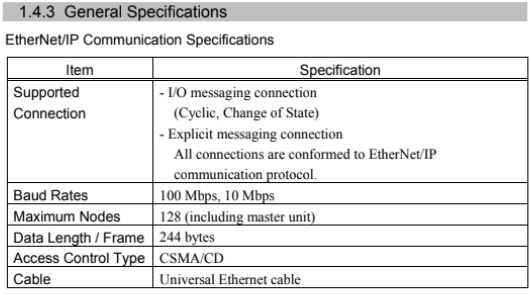
\includegraphics[width=\linewidth]{fig/fig16}
\end{figure}
\clearpage

\section{PROFINET}
PROFINET (Process Field Network) er en moderne, industrielt netværksprotokol, der muliggør hurtig og pålidelig kommunikation mellem automatiseringskomponenter, såsom PLC'er, sensorer, aktuatorer og HMI'er. PROFINET er udviklet som en efterfølger til ProfiBus, med fokus på Ethernet-baseret kommunikation og støtte til realtidsdataudveksling i komplekse industrielle miljøer.

\subsection{Introduktion}
PROFINET er designet til at imødekomme kravene i moderne automatiseringssystemer, hvor der er behov for højhastighedskommunikation, integration med IT-systemer og understøttelse af avancerede funktioner som sikkerhed og trådløs kommunikation. Protokollen gør det muligt at forbinde og styre en bred vifte af industrielle enheder i realtid, hvilket gør den ideel til både fabriksautomatisering og processtyring.

\subsection{PROFINET Protocol Stack}
PROFINET-protokollen er opdelt i flere lag, der hver især håndterer forskellige aspekter af kommunikationen. Denne strukturerede tilgang sikrer, at forskellige funktioner kan integreres og udføres effektivt inden for det samme netværk.

\subsection*{Fysisk Lag (Layer 1)}
Det fysiske lag i PROFINET er baseret på standard Ethernet-teknologi, hvilket betyder, at det understøtter standardiserede Ethernet-kabler og stik (f.eks. Cat5e, Cat6) og tilbyder høj båndbredde og fleksibilitet i netværksdesign. Dette lag specificerer også kravene til signalering og elektriske egenskaber.

\subsection*{Datalink Lag (Layer 2)}
Datalink-laget i PROFINET bygger på Ethernet MAC-laget, men tilføjer protokoltilpasninger, der understøtter realtidskommunikation (RT) og isokron realtidskommunikation (IRT). Dette lag håndterer pålidelig datatransmission, fejldetektion, adressering af enheder og datarammer.

\subsection*{Applikationslag}
Applikationslaget i PROFINET omfatter protokoller og tjenester, der er nødvendige for at implementere specifikke funktioner såsom procesdataudveksling, alarmer og diagnostik. Dette lag er også ansvarligt for konfiguration og parameterisering af enhederne på netværket.

\subsection*{Real-Time Communication (RT)}
RT-funktionen i PROFINET muliggør overførsel af procesdata med minimal latenstid, hvilket er afgørende for tidskritiske applikationer. RT kan håndtere periodiske og applikationsbestemte cykliske dataoverførsler.

\subsection*{Isocronous Real-Time Communication (IRT)}
IRT er en avanceret funktion i PROFINET, der gør det muligt at synkronisere dataoverførsel med en meget præcis timing, hvilket er nødvendigt i applikationer som motion control, hvor selv små forsinkelser kan føre til fejl.

\subsection{PROFINET Kommunikationsmodel}
PROFINET kommunikationsmodellen beskriver, hvordan data udveksles mellem enheder på netværket, inklusive de forskellige kommunikationscyklusser og dataoverførselshastigheder. Modellen understøtter både realtids- og ikke-realtidskommunikation, hvilket gør det muligt at kombinere proces- og konfigurationsdata på samme netværk.

\subsection{Forhold mellem Applikationsproces og Kommunikation}
Dette afsnit forklarer, hvordan applikationsprocesser interagerer med PROFINET-kommunikationsprotokollen for at sikre effektiv dataudveksling. Det beskriver, hvordan data struktureres og sendes mellem forskellige lag i protokolstacken for at opnå optimal kommunikationsperformance.

\subsection{Kommunikationsobjekter}
Kommunikationsobjekter i PROFINET refererer til de enheder, data og tjenester, der adresseres og styres over netværket. Dette afsnit inkluderer en beskrivelse af forskellige typer af kommunikationsobjekter, såsom input/output-data, alarmer og diagnostikbeskeder, og deres anvendelse i forskellige scenarier.

\subsection{Ydeevne}
Dette afsnit diskuterer ydeevnen af PROFINET-netværket, herunder dataoverførselshastigheder, latenstider og netværkskapacitet. Det indeholder også retningslinjer for optimering af netværkets ydeevne og sikring af, at systemet kan håndtere både realtids- og isokron dataoverførsel.

\subsection{Systemoperation}
\subsection*{Konfiguration}
Korrekt konfiguration er afgørende for at sikre, at PROFINET-netværket fungerer optimalt. Dette afsnit beskriver trinene til at konfigurere enheder, tildele IP-adresser og opsætte PROFINET-parametre, såsom cyklustider og prioriteter for forskellige datatyper.

\subsection*{Dataoverførsel mellem PLC'er og Enheder}
Dette afsnit beskriver, hvordan data overføres mellem PLC'er og de tilsluttede enheder på netværket. Det inkluderer beskrivelser af cyklisk og acyklisk dataoverførsel samt metoder til at sikre pålidelig dataudveksling.

\subsection*{Synkronisering og Timing}
Synkronisering og timing er centrale elementer i PROFINET-netværk, især i applikationer, der kræver præcis timing og koordinering mellem enheder. Dette afsnit forklarer, hvordan IRT og andre synkroniseringsmetoder implementeres i PROFINET.

\subsection*{Sikkerhed og Netværksbeskyttelse}
Sikkerhed i PROFINET-netværk er kritisk for at beskytte mod fejl og uautoriseret adgang. Dette afsnit beskriver de sikkerhedsforanstaltninger, der implementeres i PROFINET, såsom adgangskontrol, dataautentificering og kryptering.

\subsection*{Integration med IT-systemer}
Et af PROFINET's styrker er dets evne til at integrere med eksisterende IT-systemer. Dette afsnit beskriver, hvordan PROFINET kan anvendes sammen med enterprise-netværk, SCADA-systemer og andre IT-platforme for at skabe en fuldt integreret industriel løsning.

\subsection{Fejlfinding}
\subsection*{Introduktion}
Fejlfinding i et PROFINET-netværk er en essentiel del af vedligeholdelsen. Dette afsnit introducerer de grundlæggende metoder og principper for fejlfinding i PROFINET-miljøer, herunder de mest almindelige problemer og deres løsninger.

\subsection*{Fejlfinding Værktøjer}
Der findes en række værktøjer til fejlfinding i PROFINET-netværk. Dette afsnit beskriver nogle af de mest anvendte værktøjer, som netværkssniffere, diagnostiske software og integrerede funktioner i TIA Portal, og hvordan de anvendes til at identificere og løse problemer.

\subsection*{Tips}
Dette afsnit giver praktiske tips til optimering og vedligeholdelse af et PROFINET-netværk. Tipsene inkluderer forebyggende foranstaltninger, overvågning af netværkets sundhed, og metoder til at undgå almindelige faldgruber i konfiguration og drift.

\subsection{Opsummering}
PROFINET er en kraftfuld og fleksibel netværksprotokol, der er designet til at opfylde de komplekse krav i moderne industrielle automatiseringssystemer. Med sin evne til at håndtere realtidskommunikation, sikkerhed og integration med IT-systemer, er PROFINET blevet en af de mest anvendte protokoller i industriens 4.0 æra. Ved at forstå de forskellige aspekter af PROFINET, fra protokolstacken til fejlfinding, kan teknikere og ingeniører sikre, at deres netværk fungerer optimalt og opfylder kravene til nutidens automatiseringsudfordringer.

\section{AS-Interface (AS-i) Overview}
AS-Interface (AS-i) er en simpel og effektiv feltbusløsning designet til at forbinde sensorer og aktuatorer i automatiseringssystemer. AS-i er kendt for sin nemme installation og vedligeholdelse, hvilket gør det til et populært valg i industrielle applikationer.

\subsection{Introduktion}
AS-i blev udviklet som en økonomisk og brugervenlig måde at forbinde enheder som sensorer, aktuatorer og PLC'er (Programmable Logic Controllers). AS-i er kendetegnet ved en to-leder fladkabel teknologi, som både overfører data og leverer strøm til tilsluttede enheder. Denne enkelhed gør det muligt for AS-i at reducere omkostningerne og kompleksiteten ved installation og vedligeholdelse.

\subsection{Layer 1 – The Physical Layer}
Det fysiske lag i AS-i definerer de elektriske og mekaniske egenskaber ved netværksforbindelserne. Dette inkluderer specifikationer for kabler, stik og elektriske signaler, der bruges til at overføre data og strøm mellem enheder. AS-i bruger et fladkabelsystem, som er nemt at installere og tilslutte, hvilket minimerer fejl og reducerer installationsomkostningerne.

\subsection{Layer 2 – The Data Link Layer}
Datalink-laget håndterer pålidelig overførsel af data mellem enheder på AS-i netværket. Dette lag sikrer korrekt adressering, fejlregistrering og dataintegritet ved hjælp af cyklisk redundanskontrol (CRC). Datalink-laget koordinerer også kommunikationen mellem master- og slaveenheder, hvilket sikrer synkroniseret dataudveksling.

\subsection{Operating Characteristics}
AS-i systemet er designet til at fungere under forskellige industrielle forhold og tilbyder robusthed og pålidelighed. Nogle af de vigtigste driftskarakteristika inkluderer:
\begin{itemize}
	\item \textbf{Fejltolerance:} AS-i netværk er modstandsdygtige over for elektrisk støj og andre forstyrrelser, hvilket sikrer stabil og pålidelig kommunikation.
	\item \textbf{Modularitet:} AS-i enheder kan nemt tilføjes eller fjernes uden at forstyrre det overordnede system, hvilket giver fleksibilitet ved ændringer eller udvidelser.
	\item \textbf{Diagnosticering:} AS-i systemet inkluderer diagnosticeringsfunktioner, der gør det muligt at identificere og rette fejl hurtigt og effektivt.
\end{itemize}

\subsection{Troubleshooting}
Fejlfinding i AS-i systemer er designet til at være enkel og effektiv, takket være indbyggede diagnostikværktøjer og funktioner.

\subsection*{Introduktion}
Dette afsnit giver en introduktion til de grundlæggende principper for fejlfinding i AS-i netværk. Fejlfinding er en afgørende del af vedligeholdelsen og sikrer, at systemet fungerer korrekt og pålideligt.

\subsection*{Tools of the Trade}
Der findes flere værktøjer til rådighed for fejlfinding i AS-i systemer. Nogle af de mest anvendte værktøjer inkluderer:
\begin{itemize}
	\item \textbf{AS-i Master Monitor:} Dette værktøj bruges til at overvåge og diagnosticere kommunikationen mellem master- og slaveenheder.
	\item \textbf{Handheld Testers:} Bærbare enheder, der kan tilsluttes direkte til AS-i netværket for at udføre diagnostik og fejlfindingsopgaver.
	\item \textbf{Software Tools:} Specialiseret software, der kan bruges til at analysere netværksdata og identificere problemer.
\end{itemize}

\subsection{Opsummering}
AS-Interface (AS-i) er en effektiv og brugervenlig løsning til netværk af sensorer og aktuatorer i industrielle applikationer. Ved at forstå de forskellige lag i AS-i protokollen og have de rette værktøjer til fejlfinding, kan teknikere sikre, at deres AS-i netværk fungerer optimalt og pålideligt.

\section{IO-Link}
IO-Link er en standardiseret I/O-teknologi, der giver mulighed for kommunikation mellem sensorer og aktuatorer samt kontrolsystemer. Denne teknologi forbedrer diagnoser og parametrering af enheder, hvilket øger effektiviteten og fleksibiliteten i automatiseringssystemer.

\subsection{Purpose of Technology}
Formålet med IO-Link teknologien er at levere en åben standardiseret grænseflade til kommunikation med intelligente sensorer og aktuatorer. Dette muliggør ikke kun overførsel af procesdata, men også diagnostik og parametreringsinformation, hvilket resulterer i forbedret vedligeholdelse og procesoptimering.

\subsection{Positioning within the Automation Hierarchy}
IO-Link er placeret på det laveste niveau i automatiseringshierarkiet og fungerer som en point-to-point kommunikationsprotokol mellem en IO-Link master og forskellige IO-Link enheder. Det integreres problemfrit med eksisterende feltbusser og industrielle Ethernet-netværk, hvilket sikrer dataoverførsel fra feltniveau til kontrolniveau.

\subsection{Wiring, Connectors, and Power}
IO-Link bruger standard industrielle kabler og stik til forbindelser, hvilket gør installationen enkel og omkostningseffektiv. Et standard 3-leder kabel bruges til både data og strøm, hvilket eliminerer behovet for specialkabler og reducerer ledningsomkostningerne.

\subsection{Communication Features of IO-Link}
IO-Link kommunikationsprotokollen tilbyder flere avancerede funktioner:
\begin{itemize}
	\item \textbf{Automatisk Device Identification:} IO-Link enheder identificeres automatisk af masteren, hvilket forenkler opsætningen.
	\item \textbf{Diagnostik:} IO-Link muliggør løbende overvågning og diagnostik af enheder, hvilket hjælper med at identificere og løse problemer hurtigt.
	\item \textbf{Parametrering:} Enheder kan parametreres via IO-Link, hvilket gør det muligt at justere indstillinger uden fysisk adgang til enhederne.
\end{itemize}

\subsection{Role of a Master}
IO-Link masteren fungerer som en kommunikationshub mellem kontrolsystemet og IO-Link enhederne. Den samler data fra flere IO-Link enheder og sender dem videre til kontrolsystemet, samtidig med at den sender kontrolkommandoer til enhederne. Masteren håndterer også diagnostik og parametrering af tilsluttede enheder.

\subsection{IO-Link Configuration}
Konfiguration af IO-Link enheder udføres typisk via IO-Link masteren ved hjælp af softwareværktøjer. Disse værktøjer giver et brugervenligt interface til at indstille parametre, overvåge status og diagnosticere fejl. Konfigurationsdata kan gemmes og genanvendes, hvilket forenkler opsætning af nye enheder eller udskiftning af defekte enheder.

\subsection{Mapping to Fieldbuses and System Integration}
IO-Link kan integreres med forskellige feltbusser og industrielle Ethernet-netværk ved hjælp af gateways eller IO-Link mastere med indbyggede feltbusinterfaces. Dette muliggør problemfri dataoverførsel fra IO-Link enheder til overordnede kontrolsystemer, hvilket forbedrer dataudnyttelse og systemintegration.

\subsection{Implementation and Engineering Support}
Implementering af IO-Link teknologien understøttes af omfattende dokumentation og softwareværktøjer fra producenter og standardiseringsorganer. Disse ressourcer hjælper med design, opsætning og vedligeholdelse af IO-Link systemer. Desuden tilbyder mange leverandører teknisk support og træningsprogrammer for at sikre en vellykket implementering.

\subsection{Test and Certification}
IO-Link enheder og systemer gennemgår test og certificering for at sikre kompatibilitet og pålidelighed. Standardiseringsorganer som IO-Link Consortium tilbyder certificeringsprogrammer, der sikrer, at produkter overholder de nødvendige standarder og fungerer korrekt i forskellige anvendelser.

\subsection{Profiles}
IO-Link understøtter forskellige profiler, som definerer specifikke funktioner og parametre for forskellige typer af enheder, såsom sensorer, aktuatorer og komplekse enheder. Disse profiler sikrer standardisering og interoperabilitet mellem forskellige producenters enheder.

\subsection{Functional Safety}
IO-Link teknologien inkluderer også funktioner til funktionel sikkerhed, hvilket gør det muligt at bruge IO-Link i applikationer, hvor sikkerhed er kritisk. Dette inkluderer sikkerhedsprotokoller og redundansmekanismer, der sikrer, at systemerne fungerer sikkert og pålideligt selv under fejlforhold.

\section{KepServerEX}

\subsection{Introduktion til KepServerEX}
En kort introduktion til hvad Kepware KepServerEX er, og hvorfor det er vigtigt i industrielle applikationer.

\subsection{Hvad er KepServerEX?}
\subsection{Definition af KepServerEX}
En grundig forklaring af KepServerEX, herunder dets funktion som en industristandard OPC-server og dataintegrationsplatform.

\subsection{Historie og Udvikling}
En kort gennemgang af KepServerEX's historie og hvordan det har udviklet sig over tid.

\subsection{Markedets Position}
Diskussion om KepServerEX's rolle og position på markedet i forhold til andre lignende produkter.

\subsection{Funktioner og Kapaciteter i KepServerEX}
\subsection{Grundlæggende Funktioner}
En detaljeret gennemgang af de vigtigste funktioner i KepServerEX, såsom OPC-kommunikation, datalogging, protokolkonvertering, og sikkerhedsaspekter.

\subsection{Udvidede Funktioner}
Uddybning af avancerede funktioner som scripting, skalerbarhed, og IoT-integration.

\subsubsection{Scripting}
Hvordan scripting bruges i KepServerEX til at automatisere processer.

\subsubsection{IoT Gateways}
Brugen af IoT Gateways i KepServerEX til at integrere med industrielle IoT-enheder.

\subsection{Hvordan KepServerEX Anvendes i Industrien}
\subsection{Integration med Kontrolsystemer}
Eksempler på, hvordan KepServerEX integreres med forskellige kontrolsystemer, såsom PLC'er og DCS'er.

\subsection{Anvendelse i SCADA og MES}
Hvordan KepServerEX bruges sammen med SCADA- og MES-systemer for at forbedre produktionsprocesser.

\subsection{Eksempler fra Industrien}
Reelle eksempler på praktisk brug af KepServerEX i forskellige brancher.

\subsection{Opsætning og Konfiguration af KepServerEX}
\subsection{Installation af KepServerEX}
Trin-for-trin vejledning i installationen af KepServerEX.

\subsection{Grundlæggende Konfiguration}
Hvordan man opsætter og konfigurerer KepServerEX for at kommunikere med forskellige industrielle enheder og systemer.

\subsubsection{OPC-konfiguration}
Opsætning af OPC-kommunikation i KepServerEX.

\subsubsection{Sikkerhedsindstillinger}
Konfiguration af sikkerhedsaspekter i KepServerEX for at sikre dataintegritet og beskyttelse.

\subsection{Integration af KepServerEX med Andre Systemer}
\subsection{Integration med PLC'er}
Forklaring af, hvordan KepServerEX kan integreres med PLC-systemer.

\subsection{Integration med DCS og SCADA}
Beskrivelse af integration med DCS- og SCADA-systemer.

\subsection{Integration med Cloud-platforme}
Hvordan KepServerEX kan forbindes til cloud-platforme for dataanalyse og lagring.

\subsection{Fordele og Udfordringer ved at Bruge KepServerEX}
\subsection{Fordele}
Diskuter de fordele, KepServerEX bringer til industrielle applikationer.

\subsection{Udfordringer}
Eventuelle udfordringer eller overvejelser, der skal tages i betragtning ved brug af KepServerEX.

\subsection{Eksempler på Anvendelse af KepServerEX i Forskellige Brancher}
\subsection{Fremstillingsindustrien}
Hvordan KepServerEX bruges i fremstillingsindustrien for at forbedre produktionseffektiviteten.

\subsection{Energisektoren}
Eksempler på KepServerEX's anvendelse i energisektoren til dataovervågning og kontrol.

\subsection{Vandbehandling}
Anvendelse af KepServerEX i vandbehandlingsanlæg for at sikre kontinuerlig overvågning og styring.

\subsection{Bygningsteknologi}
Hvordan KepServerEX kan integreres i bygningsautomatiseringssystemer.

\subsection{Avancerede Funktioner i KepServerEX}
\subsection{Scripting og Automatisering}
Hvordan scripting i KepServerEX kan bruges til at automatisere komplekse processer.

\subsection{Skalerbarhed i KepServerEX}
Diskussion om skalerbarhed og hvordan KepServerEX kan tilpasses voksende netværkskrav.

\subsection{IoT-integration}
Hvordan KepServerEX understøtter integration med IoT-enheder og systemer.

\section{OPC}
\clearpage
	% Avancerede Netværksapplikationer
	\part{Opgaver}
\chapter{C++ Basic}
\section{\texttt{Delay()} i Arduino}

\subsection*{Formål}
Formålet med dette afsnit er at introducere og forklare, hvordan \texttt{delay()}-funktionen fungerer i Arduino-programmering, herunder dens fordele og ulemper, samt hvordan man kan anvende funktionen effektivt i projekter.

\subsection*{Introduktion}
\texttt{delay()} er en indbygget funktion i Arduino-programmeringssproget, der bruges til at skabe en pause i kodeudførelsen i en bestemt periode. Funktionen tager en enkelt parameter: den tid, programmet skal vente, angivet i millisekunder.

\subsection*{Hvad er \texttt{delay()}?}
\texttt{delay()}-funktionen bruges til at stoppe programudførelsen for en angivet tid, hvilket kan være nyttigt i mange situationer, såsom at blinke en LED eller skabe tidsbaserede sekvenser. Her er et eksempel på, hvordan \texttt{delay()} kan bruges til at tænde og slukke den indbyggede LED på et Arduino-board:

\begin{lstlisting}[language=C++, caption={Using the \texttt{delay()} function with the built-in LED.}]
	void setup() {
		pinMode(LED_BUILTIN, OUTPUT); 
		// Set the built-in LED as OUTPUT
	}
	
	void loop() {
		digitalWrite(LED_BUILTIN, HIGH); 
		// Turn on the built-in LED
		delay(1000);                     
		// Wait for 1000 milliseconds (1 second)
		digitalWrite(LED_BUILTIN, LOW);  
		// Turn off the built-in LED
		delay(1000);                     
		// Wait for 1000 milliseconds (1 second)
	}
\end{lstlisting}

\subsection*{Opgaver med \texttt{delay()}}

\subsubsection*{Opgave 1: Blinkende LED}
\textbf{Formål:}\\
Lær at styre den indbyggede LED på en ESP32 eller Arduino-board ved hjælp af \texttt{delay()}-funktionen.

\textbf{Opgave:}
\begin{enumerate}
	\item Tænd den indbyggede LED i 2 sekunder.
	\item Sluk den indbyggede LED i 3 sekunder.
	\item Gentag trin 1 og 2 kontinuerligt.
\end{enumerate}

\subsubsection*{Opgave 2: Sekvens af LED'er}
\textbf{Formål:}\\
Lær at styre flere LED'er sekventielt ved hjælp af \texttt{delay()}-funktionen.

\textbf{Materialer:}
\begin{itemize}
	\item 3 LED'er
	\item 3 220-ohm modstande
	\item Breadboard og jumperkabler
\end{itemize}

\textbf{Opgave:}
\begin{enumerate}
	\item Tilslut de tre LED'er til henholdsvis pin 2, 3 og 4 på dit board.
	\item Tænd LED 1 (pin 2) i 1 sekund, og sluk den derefter.
	\item Umiddelbart efter LED 1 slukker, tænd LED 2 (pin 3) i 1 sekund, og sluk den derefter.
	\item Umiddelbart efter LED 2 slukker, tænd LED 3 (pin 4) i 1 sekund, og sluk den derefter.
	\item Gentag trin 2-4 kontinuerligt.
\end{enumerate}

\subsubsection*{Opgave 3: Trafiklys-simulator}
\textbf{Formål:}\\
Simulere et trafiklys ved hjælp af \texttt{delay()}-funktionen.

\textbf{Materialer:}
\begin{itemize}
	\item Rød, gul og grøn LED
	\item 3 220-ohm modstande
	\item Breadboard og jumperkabler
\end{itemize}

\textbf{Opgave:}
\begin{enumerate}
	\item Tilslut de tre LED'er til henholdsvis pin 2 (rød), 3 (gul) og 4 (grøn) på dit board.
	\item Tænd den røde LED i 5 sekunder, og sluk den derefter.
	\item Tænd den gule LED i 1,5 sekund, og sluk den derefter.
	\item Tænd den grønne LED i 4 sekunder, og sluk den derefter.
	\item Gentag trin 2-4 kontinuerligt.
\end{enumerate}

\subsection*{Konklusion}
\texttt{delay()}-funktionen er en simpel, men kraftfuld måde at introducere tidsbaserede handlinger i dine Arduino-projekter. Selvom det er en nem måde at implementere pauser i kodeudførelsen, kan det også føre til udfordringer, såsom at blokere andre processer. I de kommende kapitler vil vi udforske alternative metoder til tidsstyring, som giver mere fleksibilitet og effektivitet.

\subsection*{Løsningsforslag}

\subsubsection*{Løsningsforslag for Opgave 1}
\begin{lstlisting}[language=C++]
	void setup() {
		pinMode(LED_BUILTIN, OUTPUT);
	}
	
	void loop() {
		digitalWrite(LED_BUILTIN, HIGH);  // Turn on the built-in LED
		delay(2000);                      // Wait for 2000 ms or 2 seconds
		digitalWrite(LED_BUILTIN, LOW);   // Turn off the built-in LED
		delay(3000);                      // Wait for 3000 ms or 3 seconds
	}
\end{lstlisting}

\subsubsection*{Løsningsforslag for Opgave 2}
\begin{lstlisting}[language=C++]
	void setup() {
		pinMode(2, OUTPUT);
		pinMode(3, OUTPUT);
		pinMode(4, OUTPUT);
	}
	
	void loop() {
		digitalWrite(2, HIGH);  
		delay(1000);                      
		digitalWrite(2, LOW);   
		
		digitalWrite(3, HIGH);  
		delay(1000);                      
		digitalWrite(3, LOW);   
		
		digitalWrite(4, HIGH);  
		delay(1000);                      
		digitalWrite(4, LOW);   
	}
\end{lstlisting}

\subsubsection*{Løsningsforslag for Opgave 3}
\begin{lstlisting}[language=C++]
	void setup() {
		pinMode(2, OUTPUT);  // Red LED
		pinMode(3, OUTPUT);  // Yellow LED
		pinMode(4, OUTPUT);  // Green LED
	}
	
	void loop() {
		digitalWrite(2, HIGH);  // Turn on red LED
		delay(5000);            // Wait for 5000 ms or 5 seconds
		digitalWrite(2, LOW);   // Turn off red LED
		
		digitalWrite(3, HIGH);  // Turn on yellow LED
		delay(1500);            // Wait for 1500 ms or 1.5 seconds
		digitalWrite(3, LOW);   // Turn off yellow LED
		
		digitalWrite(4, HIGH);  // Turn on green LED
		delay(4000);            // Wait for 4000 ms or 4 seconds
		digitalWrite(4, LOW);   // Turn off green LED
	}
\end{lstlisting}

\section{Trykknapper}
\subsubsection*{Introduktion}
Pull-up og pull-down modstande er essentielle for at sikre, at en digital indgang får en klart defineret værdi, uanset om den er åben eller kortsluttet. Dette er særligt vigtigt for at undgå tilfældige omskiftninger på grund af støj.

\subsubsection*{Pull-Up Modstand}
En pull-up modstand er forbundet til en digital indgang og Vcc. Når trykknappen ikke er aktiveret (ingen forbindelse), vil digital indgang læse "HIGH" på grund af pull-up modstanden. Når trykknappen er trykket, vil den digitale indgang læse "LOW", fordi knappen nu er kortsluttet til jorden.

\subsubsection*{Pull-Down Modstand}
Tilsvarende er en pull-down modstand forbundet til en digital indgang og jord. Når trykknappen ikke er aktiveret, vil den digitale indgang læse "LOW" på grund af pull-down modstanden. Når trykknappen er trykket, vil den digitale indgang læse "HIGH", da knappen nu er kortsluttet til Vcc.

\subsubsection*{Opgaver}
\begin{itemize}
	\item \textbf{Blinkende LED ved Tryk:} Skriv et program, hvor den indbyggede LED blinker, når trykknappen er trykket, og er slukket, når knappen ikke er trykket.
	\item \textbf{Veksling ved Tryk:} Skriv et program, hvor den indbyggede LED skifter mellem tændt og slukket hver gang trykknappen trykkes og frigives.
	\item \textbf{Tryk Tæller:} Skriv et program, der tæller antallet af gange, trykknappen er blevet trykket. Hver gang knappen trykkes, skal den indbyggede LED blinke svarende til det aktuelle antal tryk.
\end{itemize}

\subsubsection*{Konklusion}
For at sikre stabil aflæsning af trykknapper i digitale kredsløb er det vigtigt at anvende enten pull-up eller pull-down modstande. Dette eliminerer usikkerhed og sikrer, at mikrocontrolleren korrekt kan aflæse, om en knap er blevet trykket eller ej.

\clearpage

\subsection*{Løsningsforslag}

\subsubsection*{Blinkende LED ved Tryk}
Når trykknappen er trykket, skal den indbyggede LED tænde, og når den ikke er trykket, skal LED'en være slukket.
\begin{lstlisting}[language=C++]
	int buttonPin = 2;  // assume the button is connected to pin 2
	int ledPin = LED_BUILTIN;  // built-in LED
	
	void setup() {
		pinMode(buttonPin, INPUT_PULLUP);
		pinMode(ledPin, OUTPUT);
	}
	
	void loop() {
		int buttonState = digitalRead(buttonPin);
		if (buttonState == LOW) {   // If the button is pressed (due to INPUT_PULLUP)
			digitalWrite(ledPin, HIGH);
		} else {
			digitalWrite(ledPin, LOW); // If the button is not pressed
		}
	}
\end{lstlisting}

\subsubsection*{Veksling ved Tryk}
LED'en skifter mellem tændt og slukket hver gang trykknappen trykkes og frigives.
\begin{lstlisting}[language=C++]
	int buttonPin = 2;
	int ledPin = LED_BUILTIN;
	bool lastButtonState = HIGH;
	bool ledState = LOW;
	
	void setup() {
		pinMode(buttonPin, INPUT_PULLUP);
		pinMode(ledPin, OUTPUT);
	}
	
	void loop() {
		bool currentButtonState = digitalRead(buttonPin);
		
		if (currentButtonState == LOW && lastButtonState == HIGH) {
			ledState = !ledState;
			digitalWrite(ledPin, ledState);
			delay(50); // debounce
		}
		lastButtonState = currentButtonState;
	}
\end{lstlisting}

\subsubsection*{Tryk Tæller}
Hver gang knappen trykkes, blinker LED'en svarende til det aktuelle antal tryk.
\begin{lstlisting}[language=C++]
	int buttonPin = 2;
	int ledPin = LED_BUILTIN;
	bool lastButtonState = HIGH;
	int pressCount = 0;
	
	void setup() {
		pinMode(buttonPin, INPUT_PULLUP);
		pinMode(ledPin, OUTPUT);
	}
	
	void loop() {
		bool currentButtonState = digitalRead(buttonPin);
		
		if (currentButtonState == LOW && lastButtonState == HIGH) {
			pressCount++;
			for(int i = 0; i < pressCount; i++) {
				digitalWrite(ledPin, HIGH);
				delay(250);
				digitalWrite(ledPin, LOW);
				delay(250);
			}
			delay(50); // debounce
		}
		lastButtonState = currentButtonState;
	}
\end{lstlisting}
Med disse løsningsforslag vil din Arduino reagere forskelligt på trykknappens tilstand afhængigt af det specifikke program, du har valgt.

\section{DHT11 Sensor}
\subsection*{Formål}
Formålet med dette afsnit er at introducere læseren til DHT11-føleren, en prisvenlig og effektiv enhed til måling af temperatur og luftfugtighed. Ved at kombinere teoretisk viden med praktisk anvendelse vil læseren få hands-on erfaring med at opsætte, programmere og aflæse data fra DHT11 ved hjælp af ESP32 mikrocontrolleren. De medfølgende opgaver er designet til at styrke forståelsen af, hvordan DHT11-føleren fungerer, samt hvordan data kan bearbejdes og anvendes i forskellige scenarier. Derudover inkorporeres matematiske koncepter for at styrke integrationen af programmering og matematik i realverdenen. Gennem dette afsnit vil læseren opnå en solid forståelse for både hardware- og softwareaspekterne ved at arbejde med temperatur- og fugtighedsfølere i indlejrede systemer.

\subsection*{Introduktion til DHT11-føleren}
DHT11 er en populær temperatur- og luftfugtighedsføler, som er både omkostningseffektiv og nem at bruge. Den fungerer ved at måle omgivende luft og give digitale signaler, der kan læses fra et mikrocontroller board som ESP32.

\subsection*{Opsætning af DHT11 med ESP32}
\begin{enumerate}
	\item Tilslut DHT11-følerens VCC og GND til ESP32's 3,3V og GND henholdsvis.
	\item Tilslut data-pinden fra DHT11-føleren til en valgfri GPIO-pin på ESP32.
	\item Installér det nødvendige bibliotek til DHT11 ved at benytte PlatformIO's bibliotekshåndtering eller Arduino IDE's bibliotekshåndtering.
\end{enumerate}

\subsection*{Opgaver}
\begin{itemize}
	\item \textbf{Temperature Alarm:} Write a program that turns on the built-in LED if the temperature exceeds 25 degrees Celsius.
	\item \textbf{Humidity Difference Calculator:} Given that the maximum comfortable humidity level for a person is \(X\%\), write a program that calculates the difference between the current humidity and \(X\%\) and prints this value.
	\item \textbf{Temperature Converter:} Write a program that converts the measured temperature from Celsius to Fahrenheit and prints both values.
\end{itemize}

\subsection*{Konklusion}
Gennem denne vejledning har vi dykket ned i, hvordan DHT11-føleren fungerer og kan integreres med ESP32 for at aflæse omgivelsens temperatur og fugtighed. Denne viden er afgørende for mange IoT-applikationer, især dem, der fokuserer på klimakontrol, landbrug eller generel miljøovervågning.
\newline\newline\noindent
Med korrekt integration og programmering er DHT11 en pålidelig kilde til miljødata. Kombineret med matematisk analyse har vi også set, hvordan man kan manipulere og bruge disse data til at drage konklusioner eller lave forudsigelser.
\newline\newline\noindent
For dem, der ønsker at gå videre, kan yderligere eksperimenter og udviklingsprojekter med DHT11 og andre sensorer udforske, hvordan disse teknologier kan integreres i større systemer eller anvendes til at løse specifikke tekniske udfordringer.
\subsection*{Løsningsforslag}
\begin{itemize}
	\item \textbf{Temperature Alarm:} 
	\begin{lstlisting}[language=C++]
		#include <DHT.h>
		#define DHTPIN <Your GPIO pin>
		#define DHTTYPE DHT11
		DHT dht(DHTPIN, DHTTYPE);
		
		void setup() {
			dht.begin();
			pinMode(LED_BUILTIN, OUTPUT);
		}
		
		void loop() {
			float temp = dht.readTemperature();
			if (temp > 25) {
				digitalWrite(LED_BUILTIN, HIGH);
			} else {
				digitalWrite(LED_BUILTIN, LOW);
			}
		}
	\end{lstlisting}
	
	\item \textbf{Humidity Difference Calculator:}
	\begin{lstlisting}[language=C++]
		#include <DHT.h>
		#define DHTPIN <Your GPIO pin>
		#define DHTTYPE DHT11
		#define MAX_HUMIDITY X
		DHT dht(DHTPIN, DHTTYPE);
		
		void setup() {
			dht.begin();
			Serial.begin(9600);
		}
		
		void loop() {
			float humidity = dht.readHumidity();
			float diff = humidity - MAX_HUMIDITY;
			Serial.println(diff);
			delay(2000);
		}
	\end{lstlisting}
	
	\item \textbf{Temperature Converter:} 
	\begin{lstlisting}[language=C++]
		#include <DHT.h>
		#define DHTPIN <Your GPIO pin>
		#define DHTTYPE DHT11
		DHT dht(DHTPIN, DHTTYPE);
		
		void setup() {
			dht.begin();
			Serial.begin(9600);
		}
		
		void loop() {
			float tempC = dht.readTemperature();
			float tempF = tempC * 1.8 + 32;
			Serial.print("Temperature in C: "); Serial.println(tempC);
			Serial.print("Temperature in F: "); Serial.println(tempF);
			delay(2000);
		}
	\end{lstlisting}
\end{itemize}

\section{PIR Sensors}

\subsection*{Formål}
Formålet med dette afsnit er at introducere læseren til PIR-sensorer, en pålidelig teknologi til detektion af bevægelse baseret på infrarød stråling. Vi vil undersøge, hvordan PIR-sensorer arbejder, hvordan de kan integreres med ESP32 mikrocontrolleren, og hvordan de anvendes i praksis for at skabe bevægelsesaktiverede systemer. Dette vil suppleres med en række opgaver, der kombinerer tekniske og matematiske koncepter for at forstærke forståelsen af dette område.

\subsection*{Introduktion til PIR-sensorer}
En PIR-sensor (Passive Infrared-sensor) er en elektronisk sensor, der måler infrarødt (IR) lys, som udsendes fra genstande i dens synsfelt. De mest almindeligt anvendte typer af PIR-sensorer bruges i bevægelsesdetekteringssystemer som alarmer og belysning.

\subsection*{Opsætning af PIR-sensor med ESP32}
\begin{enumerate}
	\item Tilslut PIR-sensorens VCC og GND til ESP32's 3,3V og GND henholdsvis.
	\item Tilslut data-pinden fra PIR-sensoren til en valgfri GPIO-pin på ESP32.
	\item Initialiser GPIO-pinden i INPUT-tilstand i din kode.
\end{enumerate}

\subsection*{Opgaver}
\begin{itemize}
	\item \textbf{Motion Alarm:} Write a program that turns on the built-in LED if motion is detected by the PIR sensor.
	\item \textbf{Motion Time Calculator:} Record the time of the last five detected motions. Calculate the time intervals between them and print the average.
	\item \textbf{Alarm Counter:} Write a program that counts the number of times motion is detected within a given time period, such as 10 minutes.
\end{itemize}

\subsection*{Konklusion}
PIR-sensorer er essentielle i mange IoT- og automatiseringsprojekter, hvor bevægelsesdetektering er nødvendig. Ved korrekt integration med ESP32 kan man skabe intelligente systemer, der reagerer på menneskelig eller dyrisk bevægelse. Gennem denne vejledning og de tilhørende opgaver skulle læseren gerne have opnået en solid forståelse for, hvordan man opsætter, programmerer og drager nytte af PIR-sensorer.

\clearpage

\subsection*{Løsningsforslag}

\subsubsection*{Motion Alarm}
The built-in LED should turn on when motion is detected and turn off when no motion is detected.
\begin{lstlisting}[language=C++]
	#define PIRPIN <Your GPIO pin>
	void setup() {
		pinMode(PIRPIN, INPUT);
		pinMode(LED_BUILTIN, OUTPUT);
	}
	void loop() {
		int pirState = digitalRead(PIRPIN);
		if (pirState == HIGH) {
			digitalWrite(LED_BUILTIN, HIGH);
		} else {
			digitalWrite(LED_BUILTIN, LOW);
		}
	}
\end{lstlisting}

\subsubsection*{Motion Time Calculator}
This program records the time of the last five detected motions and calculates the average time interval between them.
\begin{lstlisting}[language=C++]
	#define PIRPIN <Your GPIO pin>
	unsigned long lastDetectedTimes[5] = {0, 0, 0, 0, 0};
	int currentIndex = 0;
	
	void setup() {
		pinMode(PIRPIN, INPUT);
		Serial.begin(9600);
	}
	
	void loop() {
		int pirState = digitalRead(PIRPIN);
		if (pirState == HIGH) {
			unsigned long currentTime = millis();
			lastDetectedTimes[currentIndex] = currentTime;
			currentIndex = (currentIndex + 1) % 5;
			
			unsigned long intervalSum = 0;
			for (int i = 1; i < 5; i++) {
				intervalSum += (lastDetectedTimes[i] - lastDetectedTimes[i - 1]);
			}
			float averageInterval = intervalSum / 4.0;
			Serial.println("Average interval: " + String(averageInterval) + " ms");
			delay(1000);  // Wait to avoid multiple detections
		}
	}
\end{lstlisting}

\subsubsection*{Alarm Counter}
This program counts the number of times motion is detected within a given time period, such as 10 minutes.
\begin{lstlisting}[language=C++]
	#define PIRPIN <Your GPIO pin>
	unsigned long startTime;
	int movementCount = 0;
	const unsigned long TEN_MINUTES = 10 * 60 * 1000;
	
	void setup() {
		pinMode(PIRPIN, INPUT);
		Serial.begin(9600);
		startTime = millis();
	}
	
	void loop() {
		if (millis() - startTime >= TEN_MINUTES) {
			Serial.println("Number of motions in the last 10 minutes: " + String(movementCount));
			movementCount = 0;
			startTime = millis();
		}
		
		int pirState = digitalRead(PIRPIN);
		if (pirState == HIGH) {
			movementCount++;
			delay(1000);  // Wait to avoid multiple detections
		}
	}
\end{lstlisting}

\section{RFID Teknologi}

\subsection*{Formål}
Formålet med dette afsnit er at introducere læseren for RFID-teknologi og den typiske anvendelse af en RFID-kortlæser, som MFRC522, sammen med en ESP32-mikrocontroller. Afsnittet giver en dybdegående forståelse af, hvordan man kan programmere og interagere med RFID-tags ved hjælp af ESP32, og hvordan disse tags kan bruges i daglige applikationer som adgangskontrol, identifikation og sporing.

\subsection*{Introduktion til RFID Kortlæseren}
RFID står for Radio Frequency Identification. Med RFID kan man trådløst identificere og spore tags, der er fastgjort til objekter. Kortlæseren, som MFRC522, bruger elektromagnetiske felter til automatisk at identificere og spore tags, som indeholder lagret information.

\subsection*{Opsætning af MFRC522 med ESP32}
\begin{enumerate}
	\item Tilslut MFRC522's VCC, RST, GND til ESP32's 3,3V, valgfri RESET pin og GND henholdsvis.
	\item Tilslut MISO, MOSI, SCK og SDA (SS) til ESP32's relevante SPI-pins.
	\item Installér det nødvendige bibliotek (f.eks., MFRC522 library) via PlatformIO eller Arduino IDE.
\end{enumerate}

\subsection*{Opgaver}
\begin{itemize}
	\item \textbf{Basic Card Reading:} Write a program that reads an RFID tag and prints its unique ID (UID) to the serial monitor.
	\item \textbf{Access Control:} Design a system where only specific RFID tags can turn on an LED. All other tags should turn off the LED.
	\item \textbf{Card Reading with Time:} Write a program that prints the exact time an RFID tag was scanned.
\end{itemize}

\subsection*{Konklusion}
Med denne vejledning har vi opnået grundlæggende viden om RFID-teknologi og dens mange applikationer, specifikt ved at integrere MFRC522-kortlæseren med ESP32-mikrocontrolleren. Teknologien bag RFID kan drastisk forbedre automatiserings- og identifikationsprocesserne i mange industrier, og forståelsen af dens grundlæggende funktionsmåde er essentiel for moderne elektronikentusiaster og ingeniører.

\clearpage

\subsection*{Løsningsforslag}
Her er løsningsforslagene til de stillede opgaver:

\subsubsection*{Basic Card Reading}

\begin{lstlisting}[language=C++, caption=Basic Card Reading Solution]
	#include <MFRC522.h>
	
	MFRC522 mfrc522(SS_PIN, RST_PIN);  // Create MFRC522 instance
	
	void setup() {
		Serial.begin(9600);
		SPI.begin();
		mfrc522.PCD_Init();
	}
	
	void loop() {
		if (!mfrc522.PICC_IsNewCardPresent()) return;
		if (!mfrc522.PICC_ReadCardSerial()) return;
		
		Serial.print("RFID tag UID:");
		for (byte i = 0; i < mfrc522.uid.size; i++) {
			Serial.print(mfrc522.uid.uidByte[i] < 0x10 ? " 0" : " ");
			Serial.print(mfrc522.uid.uidByte[i], HEX);
		}
		Serial.println();
	}
\end{lstlisting}

\subsubsection*{Access Control}

\begin{lstlisting}[language=C++, caption=Access Control Solution]
	#include <MFRC522.h>
	
	#define LED_PIN 13  // LED pin
	
	MFRC522 mfrc522(SS_PIN, RST_PIN);  // Create MFRC522 instance
	
	void setup() {
		Serial.begin(9600);
		pinMode(LED_PIN, OUTPUT);
		SPI.begin();
		mfrc522.PCD_Init();
	}
	
	void loop() {
		if (!mfrc522.PICC_IsNewCardPresent()) return;
		if (!mfrc522.PICC_ReadCardSerial()) return;
		
		// Example of a valid tag UID
		byte validUID[] = {0x12, 0x34, 0x56, 0x78};
		
		bool isValid = true;
		for (byte i = 0; i < mfrc522.uid.size; i++) {
			if (mfrc522.uid.uidByte[i] != validUID[i]) {
				isValid = false;
				break;
			}
		}
		
		if (isValid) {
			digitalWrite(LED_PIN, HIGH);  // Turn on LED
		} else {
			digitalWrite(LED_PIN, LOW);   // Turn off LED
		}
	}
\end{lstlisting}

\clearpage
\subsubsection*{Card Reading with Time}

\begin{lstlisting}[language=C++, caption=Card Reading with Time Solution]
	#include <MFRC522.h>
	
	MFRC522 mfrc522(SS_PIN, RST_PIN);  // Create MFRC522 instance
	
	void setup() {
		Serial.begin(9600);
		SPI.begin();
		mfrc522.PCD_Init();
	}
	
	void loop() {
		if (!mfrc522.PICC_IsNewCardPresent()) return;
		if (!mfrc522.PICC_ReadCardSerial()) return;
		
		Serial.print("RFID tag UID:");
		for (byte i = 0; i < mfrc522.uid.size; i++) {
			Serial.print(mfrc522.uid.uidByte[i] < 0x10 ? " 0" : " ");
			Serial.print(mfrc522.uid.uidByte[i], HEX);
		}
		Serial.print(" scanned at time ");
		Serial.println(millis() / 1000);  // Outputs time in seconds since program started
	}
\end{lstlisting}

\section{Servo Motor Teknologi}

\subsection*{Formål}
Formålet med dette afsnit er at introducere læseren for servo motor teknologi og den typiske anvendelse af en servo motor i kombination med en mikrocontroller som Arduino. Afsnittet giver en dybdegående forståelse af, hvordan man kan programmere og interagere med en servo motor ved hjælp af Arduino, og hvordan disse kan bruges i forskellige applikationer som robotter, fjernstyrede køretøjer og mere.

\subsection*{Introduktion til Servo Motorer}
En servo motor er en type motor, der kan bevæge sig eller dreje et objekt til en specifik vinkel eller afstand. Den bruges ofte i robotteknik, fjernstyrede biler, fly og andre applikationer, hvor præcis bevægelse er nødvendig. Servoer styres normalt ved hjælp af et pulsbreddemodulation (PWM) signal, hvor længden af pulsen bestemmer vinklen, som servo motoren skal bevæge sig til.

\subsection*{Opsætning af Servo Motor med Arduino}
\begin{enumerate}
	\item Tilslut servo motorens signal pin til en PWM-kompatibel pin på Arduino.
	\item Tilslut servo motorens strøm og jord til henholdsvis Arduino's 5V og GND pins.
	\item Inkludér \texttt{Servo} biblioteket i din Arduino kode.
\end{enumerate}

\subsection*{Eksempelkode}
Herunder finder du en simpel kode, der demonstrerer, hvordan man kan styre en servo motor med en Arduino:

\begin{lstlisting}[language=C++, caption=Arduino Code for Controlling a Servo Motor]
	#include <Servo.h>
	
	Servo myServo;  
	int servoPin = 9; 
	
	void setup() {
		myServo.attach(servoPin);  
		myServo.write(90);  
	}
	
	void loop() {
		for (int position = 0; position <= 180; position += 1) {
			myServo.write(position);
			delay(15);
		}
		for (int position = 180; position >= 0; position -= 1) {
			myServo.write(position);
			delay(15);  
		}
	}
\end{lstlisting}

\subsection*{Opgaver}
\begin{itemize}
	\item \textbf{Basic Servo Control:} Set up a servo motor with an Arduino and program it to move from 0 to 180 degrees and back again in a continuous loop.
	\item \textbf{Servo Position Control with Potentiometer:} Connect a potentiometer to your Arduino and use it to control the position of your servo. The servo's angle should change in real-time based on the potentiometer's position.
	\item \textbf{Interactive Servo Control:} Design a simple system where a user can input a desired angle (between 0 and 180 degrees) via a computer, and the Arduino adjusts the servo's angle accordingly.
\end{itemize}

\subsection*{Konklusion}
Med denne vejledning har vi opnået grundlæggende viden om servo motor teknologi og dens mange applikationer, specifikt ved at integrere en servo motor med en Arduino mikrocontroller. Teknologien bag servo motorer kan drastisk forbedre præcision og kontrol i mange mekaniske systemer, og forståelsen af dens grundlæggende funktionsmåde er essentiel for moderne teknologi entusiaster.

\subsection*{Løsningsforslag}
\subsubsection*{Basic Servo Control}
For at opsætte en servo motor med en Arduino og få den til at bevæge sig mellem 0 og 180 grader, kan følgende kode anvendes:

\begin{lstlisting}[language=C++, caption=Basic Servo Motor Control]
	#include <Servo.h>
	
	Servo myServo;  
	int servoPin = 9;
	
	void setup() {
		myServo.attach(servoPin);
		myServo.write(90);  
	}
	
	void loop() {
		for (int position = 0; position <= 180; position++) {
			myServo.write(position);
			delay(15);
		}
		for (int position = 180; position >= 0; position--) {
			myServo.write(position);
			delay(15);
		}
	}
\end{lstlisting}
\clearpage
\subsubsection*{Servo Position Control with Potentiometer}
Ved at forbinde et potentiometer kan vi anvende følgende kode til at styre servoens vinkel:

\begin{lstlisting}[language=C++, caption=Controlling Servo Motor with Potentiometer]
	#include <Servo.h>
	
	Servo myServo;  
	int servoPin = 9;
	int potPin = A0;
	
	void setup() {
		myServo.attach(servoPin);
	}
	
	void loop() {
		int potValue = analogRead(potPin);
		int servoPos = map(potValue, 0, 1023, 0, 180);
		myServo.write(servoPos);
		delay(15);
	}
\end{lstlisting}
\clearpage
\subsubsection*{Interactive Servo Control}
For at tillade brugeren at indtaste en ønsket vinkel fra en computer, kan en simpel kommunikation mellem computeren og Arduinoen oprettes:

\begin{lstlisting}[language=C++, caption=Interactive Servo Motor Control]
	#include <Servo.h>
	
	Servo myServo;
	int servoPin = 9;
	
	void setup() {
		myServo.attach(servoPin);
		Serial.begin(9600);
	}
	
	void loop() {
		if (Serial.available()) {
			int angle = Serial.parseInt();
			if (angle >= 0 && angle <= 180) {
				myServo.write(angle);
			}
		}
	}
\end{lstlisting}
Brugeren kan nu indtaste ønskede vinkler mellem 0 og 180 grader via Arduino IDE's Serial Monitor for at styre servo motor positionen.

\section{Introduktion for ESP32 og Functions i Programmering}

\subsection*{Formål}
Formålet med dette afsnit er at introducere læseren til ESP32 mikrocontrolleren og dens funktioner. Vi vil dykke ned i, hvordan man opretter og bruger funktioner i ESP32 programmering for at optimere og strukturere kode effektivt.

\subsection*{Introduktion}
ESP32 er en serie af lavpris, lavstrøms mikrocontrollere med integreret Wi-Fi og dual-mode Bluetooth. Med et stort sæt af onboard funktioner og muligheder er ESP32 en fleksibel og omkostningseffektiv løsning til mange IoT-projekter.

\subsection*{Funktioner i Programmering}
Funktioner er et fundamentalt koncept i programmering, der giver os mulighed for at organisere og strukturere kode. Ved at opdele komplekse programmer i mindre, genanvendelige dele kan vi forbedre kodeforståelsen, genanvende kode, og gøre fejlfinding lettere.

\subsection*{Eksempel på Funktion i ESP32 Programmering}

\begin{lstlisting}[language=C++, caption=Using a function in ESP32 code]
	void setup() {
		Serial.begin(115200);
	}
	
	void loop() {
		printHello();
		delay(1000);
	}
	
	void printHello() {
		Serial.println("Hello from ESP32!");
	}
\end{lstlisting}

\subsection*{Opgaver}
\begin{itemize}
	\item \textbf{Basic Function:} Write a function that calculates the sum of two numbers and returns the result.
	\item \textbf{Temperature Conversion:} Write a function that converts Celsius to Fahrenheit.
	\item \textbf{Blink LED:} Use functions to blink an LED connected to the ESP32.
\end{itemize}

\subsection*{Konklusion}
Med forståelse af ESP32 og brugen af funktioner i programmering, kan vi skabe effektive, organiserede og genanvendelige programmer. Funktioner er hjørnestenen i struktureret programmering og er afgørende for at skabe skalerbare og vedligeholdelige systemer.

\clearpage

\subsection*{Løsningsforslag}

\subsubsection*{Basic Function}
\begin{lstlisting}[language=C++, caption=Sum function]
	int sum(int a, int b) {
		return a + b;
	}
\end{lstlisting}

\subsubsection*{Temperature Conversion}
\begin{lstlisting}[language=C++, caption=Celsius to Fahrenheit]
	float celsiusToFahrenheit(float celsius) {
		return (celsius * 9/5) + 32;
	}
\end{lstlisting}

\subsubsection*{Blink LED}
\begin{lstlisting}[language=C++, caption=Blink LED using functions]
	const int ledPin = 2; 
	
	void setup() {
		pinMode(ledPin, OUTPUT);
	}
	
	void loop() {
		blinkLED();
		delay(1000);
	}
	
	void blinkLED() {
		digitalWrite(ledPin, HIGH);
		delay(500);
		digitalWrite(ledPin, LOW);
	}
\end{lstlisting}
\clearpage
\chapter{Node-RED}
\section{Node-RED Opgaver med ESP32 Plus og Seriel Kommunikation}

\subsection{Formål}
Formålet med dette afsnit er at demonstrere, hvordan Node-RED kan anvendes til at styre og overvåge enheder via seriel kommunikation. Vi vil skabe forskellige Node-RED flows, som kommunikerer med fysiske enheder som ESP32 Plus, for at udføre simple opgaver som styring af LED'er, temperaturalarmer og servo motorer.

\subsection{Opgave 1: Aflæsning af Data fra ESP32 Plus}
Denne opgave består i at opsætte et Node-RED flow, som modtager data fra en ESP32 Plus via seriel kommunikation og viser disse data på et dashboard.
\newline\newline\noindent
\textbf{Node-RED Flow:}
\begin{enumerate}
	\item Brug en \texttt{serial in} node til at læse data fra ESP32 Plus.
	\item Brug en \texttt{function} node til at behandle dataene, hvis nødvendigt.
	\item Vis dataene på et Node-RED Dashboard ved hjælp af \texttt{text} eller \texttt{gauge} nodes.
\end{enumerate}
\textbf{GPIO-forbindelse:} Ingen specifikke GPIO'er er nødvendige for denne opgave, da den omhandler seriel kommunikation.

\subsection{Opgave 2: Afsendelse af Data til ESP32 Plus}
Denne opgave kræver, at du opsætter et Node-RED flow, som sender data fra Node-RED til ESP32 Plus via seriel kommunikation.
\newline\newline\noindent
\textbf{Node-RED Flow:}
\begin{enumerate}
	\item Brug en \texttt{text input} node på dashboardet for at tillade brugeren at indtaste data.
	\item Brug en \texttt{serial out} node til at sende de indtastede data til ESP32 Plus.
	\item Tilslut en \texttt{button} node til at udløse afsendelsen af dataene.
\end{enumerate}
\textbf{GPIO-forbindelse:} Ingen specifikke GPIO'er er nødvendige for denne opgave, da den omhandler seriel kommunikation.

\subsection{Opgave 3: Temperatur- og Fugtighedsovervågning med DHT11}
\textbf{Opgavebeskrivelse:} \\
I denne opgave skal du opsætte en DHT11-sensor til at sende temperatur- og fugtighedsdata til Node-RED via seriel kommunikation. Node-RED vil behandle disse data og vise dem på et dashboard.
\subsection{Materialer}
\begin{itemize}
	\item DHT11 temperatur- og fugtighedssensor
	\item ESP32 Plus mikrocontroller
	\item Node-RED
\end{itemize}

\subsection{Instruktioner}
\begin{enumerate}
	\item Tilslut DHT11-sensoren til ESP32 Plus. Forbind VCC til 3.3V, GND til GND, og data-pinden til GPIO 22.
	\item Upload en kode til ESP32 Plus, der læser data fra DHT11 og sender dem via seriel kommunikation.
	\item Opret et Node-RED flow, der modtager serielle data fra ESP32 Plus.
	\item Brug \texttt{function} nodes i Node-RED til at adskille temperatur- og fugtighedsdata.
	\item Vis dataene på et Node-RED Dashboard ved hjælp af \texttt{gauge} eller \texttt{chart} nodes.
\end{enumerate}

\noindent\textbf{GPIO-forbindelse:}
\begin{itemize}
	\item \textbf{VCC:} 3.3V
	\item \textbf{GND:} GND
	\item \textbf{Data:} GPIO 22
\end{itemize}

\subsection{Opgave 4: Tænd/Sluk af en Fan}
\textbf{Opgavebeskrivelse:} \\
I denne opgave skal du opsætte et Node-RED flow, som styrer en Fan baseret på data modtaget fra ESP32 Plus.

\subsection{Materialer}
\begin{itemize}
	\item Fan
	\item ESP32 Plus mikrocontroller
	\item Node-RED
\end{itemize}

\subsection{Instruktioner}
\begin{enumerate}
	\item Tilslut Fan til ESP32 Plus. Forbind den til GPIO 14 via en transistor for at styre strømmen.
	\item Upload en kode til ESP32 Plus, som modtager kommandoer fra Node-RED via seriel kommunikation og styrer Fan.
	\item Opret et Node-RED flow, der sender kommandoer til ESP32 Plus for at tænde/slukke for Fan.
	\item Brug en \texttt{switch} node til at beslutte, hvornår Fan skal aktiveres.
\end{enumerate}

\noindent\textbf{GPIO-forbindelse:}
\begin{itemize}
	\item \textbf{VCC:} 5V eller 12V afhængig af Fan specifikationer
	\item \textbf{GND:} GND
	\item \textbf{Control:} GPIO 14 (via transistor)
\end{itemize}

\subsection{Opgave 5: Temperatur Alarm med DHT11}
Denne opgave kræver, at du overvåger temperaturen og tænder en LED, hvis temperaturen overstiger en forudbestemt værdi.
\newline\newline\noindent
\textbf{Node-RED Flow:}
\begin{enumerate}
	\item Brug en \texttt{serial in} node til at modtage temperaturdata fra DHT11 sensoren tilsluttet GPIO 22.
	\item Tilslut denne node til en \texttt{switch} node, der sammenligner temperaturen med en tærskelværdi.
	\item Hvis temperaturen er over tærskelværdien, send en kommando til en \texttt{serial out} node for at tænde LED'en, som er tilsluttet GPIO 16.
\end{enumerate}
\noindent
\textbf{GPIO-forbindelse:}
\begin{itemize}
	\item \textbf{VCC:} 3.3V (for DHT11)
	\item \textbf{GND:} GND (for DHT11 og LED)
	\item \textbf{Data:} GPIO 22 (for DHT11)
	\item \textbf{LED:} GPIO 16 (via modstand)
\end{itemize}

\subsection{Opgave 6: Servo Motor Position Control}
Denne opgave kræver, at du styrer en servo motors position via data sendt fra Node-RED.
\newline\newline\noindent
\textbf{Node-RED Flow:}
\begin{enumerate}
	\item Brug en \texttt{dashboard} \texttt{slider} eller \texttt{text input} node til at vælge eller indtaste servoens vinkel.
	\item Tilslut denne node til en \texttt{serial out} node for at sende den valgte vinkel til servo motoren, som er tilsluttet GPIO 13.
\end{enumerate}
\noindent
\textbf{GPIO-forbindelse:}
\begin{itemize}
	\item \textbf{VCC:} 5V
	\item \textbf{GND:} GND
	\item \textbf{Control:} GPIO 13
\end{itemize}

\subsection{Opgave 7: RFID-læser til LED kontrol}
I denne opgave skal du bruge en RFID-læser til at kontrollere en LED via seriel kommunikation. Bemærk, at RFID-læseren skal tilsluttes 3.3V for at undgå beskadigelse.
\newline\newline\noindent
\textbf{Node-RED Flow:}
\begin{enumerate}
	\item Brug en \texttt{serial in} node til at modtage UID-data fra RFID-læseren tilsluttet ESP32 Plus.
	\item Brug en \texttt{switch} node til at sammenligne UID'et med en liste over godkendte UID'er.
	\item Hvis UID'et er godkendt, send en kommando til en \texttt{serial out} node for at tænde LED'en, som er tilsluttet GPIO 16.
\end{enumerate}
\noindent
\textbf{GPIO-forbindelse:}
\begin{itemize}
	\item \textbf{VCC:} 3.3V (vigtigt: brug ikke 5V for RFID-læseren)
	\item \textbf{GND:} GND
	\item \textbf{MISO:} GPIO 19
	\item \textbf{MOSI:} GPIO 23
	\item \textbf{SCK:} GPIO 18
	\item \textbf{SS (SDA):} GPIO 5
	\item \textbf{LED:} GPIO 16
\end{itemize}

\subsection{Opgave 8: Temperaturstyret Fan}
I denne opgave skal du kombinere en DHT11-sensor og en Fan. Fan'en skal automatisk tænde, hvis temperaturen overstiger en bestemt tærskel, og slukke, når temperaturen falder under tærsklen.
\newline\newline\noindent
\textbf{GPIO-forbindelse:}
\begin{itemize}
	\item \textbf{DHT11:} GPIO 22
	\item \textbf{Fan:} GPIO 14
\end{itemize}

\subsection{Opgave 9: Temperaturstyret RGB LED}
I denne opgave skal du kombinere en DHT11-sensor og en RGB LED. RGB LED'en skal ændre farve baseret på temperaturen (f.eks. blå for lave temperaturer, grøn for moderate, og rød for høje temperaturer).
\noindent
\textbf{GPIO-forbindelse:}
\begin{itemize}
	\item \textbf{DHT11:} GPIO 22
	\item \textbf{RGB LED:} GPIO 25 (Rød), GPIO 26 (Grøn), GPIO 27 (Blå)
\end{itemize}

\subsection{Opgave 10: RFID-baseret Fan- og LED-kontrol}
I denne opgave skal du kombinere en RFID-læser, en Fan og en LED. Kun når et specifikt RFID-tag scannes, skal Fan og LED'en tændes. Andre tags skal ikke have nogen effekt.
\newline\newline\noindent
\textbf{GPIO-forbindelse:}
\begin{itemize}
	\item \textbf{RFID-læser:} Se tidligere opgave for korrekt tilslutning
	\item \textbf{Fan:} GPIO 14
	\item \textbf{LED:} GPIO 16
\end{itemize}
%	\part{Netværkssikkerhed}
%	\section{Simpel Netværkssikkerhed}

\subsection{Introduktion til Netværkssikkerhed}
Netværkssikkerhed er en afgørende del af moderne IT-miljøer. Det omfatter de strategier, politikker og teknologier, der anvendes til at beskytte netværk mod en række trusler, herunder uautoriseret adgang, dataforfalskning, og forskellige typer af cyberangreb. I takt med at flere systemer bliver forbundet til internettet, og mængden af data, der udveksles, stiger, bliver netværkssikkerhed stadigt vigtigere. Uden tilstrækkelig beskyttelse kan organisationer risikere alvorlige sikkerhedsbrud, hvilket kan resultere i tab af følsomme oplysninger, økonomiske tab, og skader på omdømmet. Dette afsnit vil introducere de grundlæggende principper for netværkssikkerhed og forklare, hvorfor det er vigtigt at beskytte netværk mod potentielle trusler.

\subsection{Grundlæggende Sikkerhedsprincipper}
Netværkssikkerhed bygger på en række centrale principper, der tilsammen danner grundlaget for et robust sikkerhedssystem. Et af de mest fundamentale principper er "defense in depth", som indebærer at anvende flere lag af beskyttelse for at minimere risikoen for, at et enkelt punkt af svaghed kan udnyttes. Ved at implementere sikkerhedsforanstaltninger på flere niveauer - såsom firewalls, adgangskontrolsystemer, og overvågning - kan man skabe en mere modstandsdygtig sikkerhedsarkitektur.
\newline\newline\noindent
Adgangskontrol er et andet vigtigt princip, der fokuserer på at sikre, at kun autoriserede brugere og enheder har adgang til netværket. Dette kan opnås gennem brug af stærke adgangskoder, multifaktorautentificering, og netværksadgangskontrolsystemer (NAC), som alle hjælper med at beskytte netværket mod uautoriseret adgang.
\newline\newline\noindent
Sikkerhed gennem design er også en kritisk tilgang, hvor sikkerhed er indarbejdet i systemet fra starten af udviklingsprocessen, snarere end at blive tilføjet som en eftertanke. Ved at tænke sikkerhed ind i designfasen kan man skabe systemer, der er mere modstandsdygtige over for angreb og lettere at beskytte.
\newline\newline\noindent
Disse grundlæggende principper arbejder sammen for at skabe en omfattende og effektiv sikkerhedsstrategi, der kan beskytte netværk mod en bred vifte af trusler.


\subsubsection{Defense in Depth}
"Defense in Depth" er et sikkerhedsprincip, der handler om at beskytte et netværk ved hjælp af flere lag af sikkerhedsforanstaltninger. I stedet for at stole på en enkelt sikkerhedsforanstaltning, som en firewall eller et adgangskontrolsystem, anvendes flere forskellige beskyttelseslag, der hver især kan forhindre eller opdage en sikkerhedstrussel.
\newline\newline\noindent
Formålet med denne lagdelte tilgang er at skabe redundans i sikkerheden, hvilket betyder, at hvis én beskyttelsesmekanisme svigter, vil andre stadig være aktive og forhindre et sikkerhedsbrud. For eksempel kan et lag bestå af perimeterbeskyttelse som firewalls og indbrudsdetektionssystemer (IDS), mens andre lag kan omfatte adgangskontrol, kryptering, og regelmæssig sikkerhedsovervågning.
\newline\newline\noindent
"Defense in Depth" beskytter også mod en bred vifte af trusler, da forskellige lag kan være designet til at modstå forskellige typer angreb, såsom malware, phishing, eller brute force-angreb. Ved at kombinere flere sikkerhedsforanstaltninger kan man sikre, at netværket er modstandsdygtigt over for både eksterne og interne trusler, hvilket giver en omfattende og robust beskyttelse.
\newline\newline\noindent
Denne tilgang kræver dog en grundig planlægning og integration af sikkerhedsværktøjer for at sikre, at alle lag arbejder sammen effektivt og uden overlap, hvilket også kan minimere risikoen for fejlslagne sikkerhedstiltag.


\subsubsection{Adgangskontrol}
Adgangskontrol er en central komponent i netværkssikkerhed, der sikrer, at kun autoriserede brugere og enheder har adgang til netværket og dets ressourcer. Adgangskontrolsystemer fungerer ved at identificere og autentificere brugere og enheder, inden de får adgang til netværket, samt ved at bestemme, hvilke ressourcer disse brugere og enheder har tilladelse til at benytte.
\newline\newline\noindent
Adgangskontrol kan implementeres på flere niveauer. Det mest grundlæggende er identifikation og autentificering, hvor en bruger eller enhed skal bevise sin identitet gennem noget, de ved (f.eks. en adgangskode), noget, de har (f.eks. en sikkerhedsnøgle), eller noget, de er (f.eks. biometriske data). Multiffaktorautentificering (MFA) kombinerer flere af disse metoder for at øge sikkerheden.
\newline\newline\noindent
Efter autentificeringen bestemmer adgangskontrolsystemet, hvilke ressourcer brugeren eller enheden kan tilgå. Dette kan ske gennem rollebaseret adgangskontrol (RBAC), hvor adgangsrettigheder tildeles baseret på brugerens rolle i organisationen, eller gennem politikbaseret adgangskontrol, hvor adgang bestemmes af foruddefinerede sikkerhedspolitikker.
\newline\newline\noindent
Adgangskontrolsystemer kan også overvåge og logge adgangsforsøg, hvilket giver administratorer mulighed for at opdage og reagere på uautoriserede adgangsforsøg eller mistænkelig aktivitet. Desuden kan netværksadgangskontrol (NAC) sikre, at enheder, der tilslutter sig netværket, opfylder visse sikkerhedskrav, som f.eks. at have opdateret antivirussoftware installeret, før de får adgang til netværket.
\newline\newline\noindent
Ved at implementere robuste adgangskontrolforanstaltninger kan organisationer sikre, at deres netværk og data kun er tilgængelige for autoriserede personer og enheder, hvilket reducerer risikoen for uautoriseret adgang og potentielle sikkerhedsbrud.


\subsection{Sikring af Netværksadgang}
Sikring af adgangen til et netværk er en afgørende del af netværkssikkerhed, da det forhindrer uautoriserede brugere og enheder i at få adgang til følsomme data og systemer. Der findes flere metoder til at beskytte netværksadgangen, som kan anvendes sammen for at skabe en stærk og pålidelig sikkerhedsbarriere.
\newline\newline\noindent
En af de mest grundlæggende metoder er brugen af stærke adgangskoder. Stærke adgangskoder bør være komplekse, bestående af en kombination af store og små bogstaver, tal og specialtegn, samt være af en tilstrækkelig længde til at gøre dem svære at gætte. Derudover bør adgangskoder opdateres regelmæssigt for at minimere risikoen for, at de bliver kompromitteret.
\newline\newline\noindent
Multifaktorautentificering (MFA) er en anden effektiv metode til at sikre netværksadgang. MFA kræver, at brugeren beviser sin identitet ved at kombinere flere former for autentificering, såsom noget de ved (en adgangskode), noget de har (en smartphone til at modtage en engangskode), og noget de er (biometrisk data som et fingeraftryk). Ved at kræve flere autentificeringsfaktorer reducerer MFA risikoen for, at en uautoriseret bruger kan få adgang, selv hvis en enkelt faktor bliver kompromitteret.
\newline\newline\noindent
Netværksadgangskontrol (NAC) er en teknologi, der sikrer, at kun autoriserede og kompatible enheder får adgang til netværket. NAC-systemer vurderer enheders sikkerhedsstatus, f.eks. om de har den nyeste antivirussoftware installeret, før de tillader dem at oprette forbindelse til netværket. Dette hjælper med at beskytte netværket mod potentielt usikre eller kompromitterede enheder.
\newline\newline\noindent
Ved at kombinere disse metoder kan organisationer opbygge en robust forsvarsmekanisme, der effektivt beskytter netværksadgangen mod uautoriserede forsøg og sikrer, at kun legitime brugere og enheder har adgang til netværksressourcer.


\subsubsection{Stærke Adgangskoder}
Stærke og komplekse adgangskoder er en af de mest grundlæggende, men alligevel vigtige, sikkerhedsforanstaltninger for at beskytte netværk og data mod uautoriseret adgang. En stærk adgangskode er typisk lang, tilfældig og består af en kombination af store og små bogstaver, tal og specialtegn. Denne kompleksitet gør det væsentligt sværere for angribere at gætte eller bruge brute force-teknikker til at finde frem til adgangskoden.
\newline\newline\noindent
Brute force-angreb er en metode, hvor en angriber systematisk prøver alle mulige kombinationer af adgangskoder, indtil den korrekte findes. Jo længere og mere kompleks en adgangskode er, desto længere tid vil det tage for et brute force-angreb at lykkes, hvilket i mange tilfælde kan gøre angrebet praktisk talt umuligt. For eksempel vil en adgangskode på 8 tegn, der kun består af små bogstaver, have langt færre mulige kombinationer end en adgangskode på 12 tegn, der inkluderer både store og små bogstaver, tal og specialtegn.
\newline\newline\noindent
Derudover bør adgangskoder opdateres regelmæssigt for at reducere risikoen for, at en kompromitteret adgangskode kan bruges over en længere periode. Det anbefales også at undgå genbrug af adgangskoder på tværs af forskellige konti og systemer, da dette øger risikoen for, at et enkelt kompromis kan give adgang til flere systemer.
\newline\newline\noindent
Ved at bruge stærke adgangskoder kan man markant forbedre netværkets sikkerhed og gøre det meget sværere for angribere at få uautoriseret adgang gennem brute force eller andre adgangskodebaserede angreb.


\subsubsection{Multifaktorautentificering (MFA)}
Multifaktorautentificering (MFA) er en sikkerhedsteknik, der kræver, at en bruger bekræfter sin identitet ved hjælp af to eller flere forskellige faktorer, før de får adgang til et netværk eller en applikation. Disse faktorer kan omfatte noget, brugeren ved (som en adgangskode), noget, brugeren har (som en sikkerhedsnøgle eller en smartphone), og noget, brugeren er (som biometrisk data såsom et fingeraftryk eller ansigtsgenkendelse).
\newline\newline\noindent
MFA fungerer ved at kombinere disse faktorer, hvilket skaber flere lag af sikkerhed. Hvis en angriber formår at stjæle en brugers adgangskode, vil de stadig ikke kunne få adgang uden også at have adgang til den anden (eller tredje) faktor, som f.eks. en engangskode sendt til brugerens telefon eller et biometrisk login. Dette reducerer risikoen for, at en kompromitteret adgangskode kan føre til et sikkerhedsbrud.
\newline\newline\noindent
MFA er især effektiv mod phishing-angreb, hvor angribere forsøger at få brugere til at afsløre deres adgangskoder, og mod brute force-angreb, hvor en angriber systematisk forsøger at gætte en adgangskode. Selv hvis adgangskoden kompromitteres, vil MFA forhindre uautoriseret adgang, da den ekstra faktor forhindrer fuldførelse af loginprocessen.
\newline\newline\noindent
Implementeringen af MFA er en af de mest anbefalede metoder til at forbedre sikkerheden på netværk, da det betydeligt øger beskyttelsen af følsomme data og systemer mod uautoriseret adgang.


\subsubsection{Netværksadgangskontrol (NAC)}
Netværksadgangskontrol (NAC) er en teknologi, der bruges til at sikre, at kun autoriserede og sikre enheder får adgang til et netværk. NAC fungerer ved at overvåge og evaluere enhedens sikkerhedsstatus, inden den tillader enheden at oprette forbindelse til netværket. Dette hjælper med at forhindre uautoriserede eller potentielt usikre enheder i at få adgang til følsomme netværksressourcer.
\newline\newline\noindent
NAC-teknologier anvender forskellige metoder til at verificere enhedens sikkerhedsstatus, herunder kontrol af, om enheden har opdateret antivirussoftware, om operativsystemet er opdateret, og om andre sikkerhedsforanstaltninger er på plads. Hvis en enhed ikke opfylder de definerede sikkerhedskriterier, kan NAC forhindre enheden i at få adgang til netværket eller begrænse dens adgang til et isoleret område, hvor den kan opdatere sin sikkerhedsstatus, før fuld adgang gives.
\newline\newline\noindent
En central funktion ved NAC er evnen til at implementere politikker, der definerer, hvilke typer enheder der kan få adgang til netværket, og hvilke ressourcer de kan tilgå baseret på deres sikkerhedsstatus. Dette kan omfatte adskillelse af gæsteenheder fra virksomhedens hovednetværk eller begrænsning af adgangen for enheder, der ikke opfylder sikkerhedskravene.
\newline\newline\noindent
NAC kan også integreres med andre sikkerhedssystemer, såsom firewalls og intrusion detection systems (IDS), for at skabe en mere omfattende sikkerhedsløsning. Ved at implementere NAC kan organisationer effektivt beskytte deres netværk mod trusler, der kommer fra usikre eller uautoriserede enheder, og sikre, at alle tilsluttede enheder overholder organisationens sikkerhedspolitikker.


\subsection{Firewall Konfiguration}
Firewalls spiller en central rolle i at beskytte netværk mod uautoriseret adgang og forskellige former for angreb ved at fungere som en barriere mellem et internt netværk og eksterne trusler. For at en firewall effektivt kan beskytte et netværk, er det afgørende, at den er korrekt konfigureret. Her er nogle vigtige konfigurationstrin, der bør følges:

\subsubsection{Definering af Firewall-Regler}
En af de første trin i firewall-konfiguration er at definere regler, der bestemmer, hvilken trafik der skal tillades eller blokeres. Disse regler er baseret på kriterier som IP-adresser, porte og protokoller. For eksempel kan man oprette en regel, der tillader HTTP-trafik (port 80) fra en bestemt IP-adresse, mens al anden trafik fra denne adresse blokeres.

\subsubsection{Implementering af Zonebaseret Sikkerhed}
Mange moderne firewalls bruger en zonebaseret tilgang, hvor netværksressourcer opdeles i forskellige sikkerhedszoner, såsom intern (trusted), ekstern (untrusted), og DMZ (demilitarized zone). Hver zone har specifikke regler for, hvordan trafik kan flyde mellem dem. For eksempel kan trafikken mellem den eksterne zone og den interne zone være stærkt begrænset, mens trafik mellem den interne zone og DMZ'en kan tillades med visse begrænsninger.

\subsubsection{Aktivering af Stateful Inspection}
Stateful inspection, også kendt som dynamic packet filtering, er en funktion, der gør det muligt for firewallen at holde styr på forbindelsestilstanden for alle netværksforbindelser, og kun tillade pakker, der er en del af en etableret forbindelse. Dette forhindrer uautoriserede pakker i at få adgang til netværket, selvom de matcher en tilladt regel.

\subsubsection{Konfiguration af Intrusion Detection and Prevention Systems (IDPS)}
Mange firewalls integrerer nu Intrusion Detection and Prevention Systems (IDPS), som kan overvåge netværkstrafik for mistænkelig aktivitet og reagere på potentielle trusler i realtid. Konfiguration af IDPS omfatter opsætning af regler for detektering af angrebsmønstre og automatiserede svar som at blokere eller advare om trusler.

\subsubsection{Opsætning af Logging og Overvågning}
Det er også vigtigt at konfigurere logging og overvågning, så alle forsøg på at tilgå netværket logges. Dette inkluderer både tilladte og blokerede forsøg, hvilket kan hjælpe med at identificere potentielle sikkerhedstrusler. Logs skal overvåges regelmæssigt, og automatiserede alarmer kan opsættes for at advare om mistænkelig aktivitet.

\subsubsection{Regelmæssig Opdatering af Firewall-Regler}
Firewall-regler bør ikke være statiske. Det er vigtigt regelmæssigt at gennemgå og opdatere reglerne for at sikre, at de stadig er relevante og effektive mod nye trusler. Dette kan inkludere tilføjelse af nye regler, opdatering af eksisterende, eller fjernelse af forældede regler.
\newline\newline\noindent
Ved at følge disse konfigurationstrin kan man sikre, at firewallen yder effektiv beskyttelse mod uautoriseret adgang og angreb, og samtidig opretholder en fleksibel og sikker netværksarkitektur.


\subsubsection{Regelbaseret Adgangskontrol}
Regelbaseret adgangskontrol er en central funktion i firewalls, hvor specifikke regler anvendes til at filtrere netværkstrafik og forhindre uautoriseret adgang til netværket. Disse regler definerer, hvilken trafik der må passere gennem firewallen baseret på forskellige kriterier som IP-adresser, protokoller, porte og andre parametre.
\newline\newline\noindent
Når en firewall modtager en datapakke, vurderer den pakken mod sine sæt af regler. Hver regel består typisk af en tilladelses- eller blokeringserklæring og de betingelser, der skal opfyldes for at reglen kan anvendes. For eksempel kan en regel være opsat til at tillade al indkommende trafik på port 443 (HTTPS) fra en bestemt IP-adresse, mens al anden trafik på denne port fra andre IP-adresser blokeres.
\newline\newline\noindent
Firewalls kan også anvende regler til at begrænse trafik mellem forskellige segmenter af et netværk, f.eks. ved at blokere trafik fra en mindre sikker zone, såsom en demilitarized zone (DMZ), til en mere sikker intern zone. Dette sikrer, at selvom en angriber får adgang til et mindre sikkert segment af netværket, kan de ikke frit bevæge sig til andre, mere kritiske dele af netværket.
\newline\newline\noindent
Regler kan også være dynamiske, hvor de ændres eller opdateres baseret på aktuelle sikkerhedstrusler eller ændringer i netværksinfrastrukturen. Dette gør det muligt for firewallen at reagere hurtigt på nye trusler og tilpasse sig til ændringer i netværkets sikkerhedsbehov.
\newline\newline\noindent
Regelbaseret adgangskontrol giver administratorer en fleksibel og kraftfuld måde at beskytte netværket på, ved at sikre, at kun autoriseret trafik får adgang, mens potentielt skadelig eller uautoriseret trafik bliver blokeret. Det er vigtigt, at disse regler bliver nøje udformet og regelmæssigt opdateret for at sikre, at de fortsat yder effektiv beskyttelse.


\subsubsection{Intrusion Detection and Prevention Systems (IDPS)}
Intrusion Detection and Prevention Systems (IDPS) er sikkerhedsløsninger, der arbejder tæt sammen med firewalls for at opdage og forhindre uautoriseret adgang til netværket. Mens firewalls primært fokuserer på at filtrere trafik baseret på foruddefinerede regler, går IDPS et skridt videre ved at overvåge netværkstrafik i realtid for mistænkelig aktivitet, og derefter træffe foranstaltninger for at blokere eller reagere på trusler.
\newline\newline\noindent
IDPS fungerer ved at analysere netværkstrafikken og sammenligne den med kendte angrebsmønstre eller usædvanlig adfærd, der kan indikere et forsøg på indtrængen. Når systemet registrerer en potentiel trussel, kan det tage forskellige former for handlinger afhængigt af, om det er konfigureret som en Intrusion Detection System (IDS) eller en Intrusion Prevention System (IPS).

\begin{itemize}
	\item Intrusion Detection System (IDS):** Når IDS registrerer en mistænkelig aktivitet, kan det udløse alarmer, sende meddelelser til administratorer, eller logge hændelsen til senere analyse. IDS fungerer således som et overvågningsværktøj, der advarer om mulige sikkerhedstrusler, men tager ikke direkte handling for at blokere angrebet.
	
	\item Intrusion Prevention System (IPS):** IPS går et skridt videre ved ikke kun at detektere trusler, men også aktivt at forhindre dem. IPS kan automatisk blokere ondsindet trafik, droppe mistænkelige pakker, eller ændre firewall-reglerne for at forhindre yderligere angreb. IPS er designet til at reagere hurtigt på trusler og minimere risikoen for skade på netværket.
\end{itemize}

Når IDPS kombineres med firewalls, opnås en stærkere sikkerhedsarkitektur. Firewallen fungerer som den første forsvarslinje ved at blokere kendte trusler og kontrollere netværkstrafikken, mens IDPS analyserer den trafik, der kommer igennem, for at opdage avancerede eller nye trusler, som firewallen muligvis ikke kan håndtere alene.
\newline\newline\noindent
Implementering af IDPS i forbindelse med firewalls sikrer, at netværket har flere lag af beskyttelse, som kan opdage og reagere på indtrængen, før de kan forårsage skade. Dette gør IDPS til et uundværligt værktøj i moderne netværkssikkerhed.


\subsection{Sikring af Trådløse Netværk}
Trådløse netværk udgør en unik sikkerhedsudfordring, da de bruger radiobølger til at transmittere data, hvilket gør dem sårbare over for aflytning og uautoriseret adgang. For at beskytte trådløse netværk er det vigtigt at implementere en række sikkerhedsforanstaltninger, der kan forhindre, at uvedkommende får adgang til netværket eller kompromitterer de data, der transmitteres.
\newline\newline\noindent
En af de mest grundlæggende sikkerhedsforanstaltninger er at anvende stærk kryptering for at beskytte data, der sendes over det trådløse netværk. Kryptering sikrer, at selv hvis data opfanges af en tredjepart, vil de være uforståelige uden den korrekte krypteringsnøgle. Derudover er det vigtigt at sikre adgangspunkterne (AP'er), som er de fysiske enheder, der transmitterer det trådløse signal, for at forhindre uautoriseret adgang til netværket.
\newline\newline\noindent
Andre vigtige sikkerhedsforanstaltninger inkluderer brugen af stærke adgangskoder, konfiguration af netværks-SSID (Service Set Identifier), og implementering af netværksadgangskontrol (NAC) for at sikre, at kun autoriserede enheder kan oprette forbindelse til netværket.
\newline\newline\noindent
Ved at kombinere disse sikkerhedsforanstaltninger kan organisationer beskytte deres trådløse netværk mod mange af de trusler, der typisk er forbundet med trådløse forbindelser, såsom aflytning, uautoriseret adgang, og datatyveri.

\subsubsection{Kryptering af Trådløse Netværk}
Kryptering er en af de vigtigste metoder til at beskytte trådløse netværk mod uautoriseret adgang og aflytning. De mest anvendte krypteringsstandarder til trådløse netværk er WPA2 (Wi-Fi Protected Access 2) og WPA3 (Wi-Fi Protected Access 3), som begge tilbyder stærk kryptering af data, der transmitteres over det trådløse netværk.

\begin{itemize}
	\item \textbf{WPA2:} WPA2 har været standarden for trådløs kryptering i mange år og bruger AES (Advanced Encryption Standard) til at sikre netværkstrafikken. AES er en robust krypteringsalgoritme, der betragtes som sikker mod de fleste kendte angreb. WPA2 kræver, at enhederne på netværket deler en fælles krypteringsnøgle, som bruges til at kryptere og dekryptere data.
	
	\item \textbf{WPA3:} WPA3 er den nyeste krypteringsstandard og blev udviklet for at adressere nogle af de sårbarheder, der er fundet i WPA2. WPA3 introducerer en række forbedringer, herunder brugen af SAE (Simultaneous Authentication of Equals), som tilbyder en mere sikker nøgleudvekslingsproces, der beskytter mod brute force-angreb. Desuden understøtter WPA3 også individuelle krypteringsnøgler til hver forbindelse, hvilket gør det endnu sværere for angribere at aflytte eller kompromittere data.
\end{itemize}

Valget af krypteringsstandard er afgørende for sikkerheden af et trådløst netværk. WPA3 tilbyder stærkere beskyttelse og bør foretrækkes, hvis det er muligt. Dog kan WPA2 stadig give tilstrækkelig beskyttelse, hvis WPA3 ikke er tilgængelig, forudsat at stærke adgangskoder anvendes, og netværket er konfigureret korrekt.
\newline\newline\noindent
Ved at anvende WPA2 eller WPA3 kan man sikre, at data, der sendes over det trådløse netværk, er beskyttet mod uautoriseret adgang og aflytning, hvilket er afgørende for at opretholde netværkets integritet og brugernes privatliv.


\subsection{Sikring af Trådløse Netværk}
Trådløse netværk udgør en unik sikkerhedsudfordring, da de bruger radiobølger til at transmittere data, hvilket gør dem sårbare over for aflytning og uautoriseret adgang. For at beskytte trådløse netværk er det vigtigt at implementere en række sikkerhedsforanstaltninger, der kan forhindre, at uvedkommende får adgang til netværket eller kompromitterer de data, der transmitteres.
\newline\newline\noindent
En af de mest grundlæggende sikkerhedsforanstaltninger er at anvende stærk kryptering for at beskytte data, der sendes over det trådløse netværk. Kryptering sikrer, at selv hvis data opfanges af en tredjepart, vil de være uforståelige uden den korrekte krypteringsnøgle. Derudover er det vigtigt at sikre adgangspunkterne (AP'er), som er de fysiske enheder, der transmitterer det trådløse signal, for at forhindre uautoriseret adgang til netværket.
\newline\newline\noindent
Andre vigtige sikkerhedsforanstaltninger inkluderer brugen af stærke adgangskoder, konfiguration af netværks-SSID (Service Set Identifier), og implementering af netværksadgangskontrol (NAC) for at sikre, at kun autoriserede enheder kan oprette forbindelse til netværket.
\newline\newline\noindent
Ved at kombinere disse sikkerhedsforanstaltninger kan organisationer beskytte deres trådløse netværk mod mange af de trusler, der typisk er forbundet med trådløse forbindelser, såsom aflytning, uautoriseret adgang, og datatyveri.

\subsubsection{Kryptering af Trådløse Netværk}
Kryptering er en af de vigtigste metoder til at beskytte trådløse netværk mod uautoriseret adgang og aflytning. De mest anvendte krypteringsstandarder til trådløse netværk er WPA2 (Wi-Fi Protected Access 2) og WPA3 (Wi-Fi Protected Access 3), som begge tilbyder stærk kryptering af data, der transmitteres over det trådløse netværk.

\begin{itemize}
	\item \textbf{WPA2:} WPA2 har været standarden for trådløs kryptering i mange år og bruger AES (Advanced Encryption Standard) til at sikre netværkstrafikken. AES er en robust krypteringsalgoritme, der betragtes som sikker mod de fleste kendte angreb. WPA2 kræver, at enhederne på netværket deler en fælles krypteringsnøgle, som bruges til at kryptere og dekryptere data.
	
	\item \textbf{WPA3:} WPA3 er den nyeste krypteringsstandard og blev udviklet for at adressere nogle af de sårbarheder, der er fundet i WPA2. WPA3 introducerer en række forbedringer, herunder brugen af SAE (Simultaneous Authentication of Equals), som tilbyder en mere sikker nøgleudvekslingsproces, der beskytter mod brute force-angreb. Desuden understøtter WPA3 også individuelle krypteringsnøgler til hver forbindelse, hvilket gør det endnu sværere for angribere at aflytte eller kompromittere data.
\end{itemize}

Valget af krypteringsstandard er afgørende for sikkerheden af et trådløst netværk. WPA3 tilbyder stærkere beskyttelse og bør foretrækkes, hvis det er muligt. Dog kan WPA2 stadig give tilstrækkelig beskyttelse, hvis WPA3 ikke er tilgængelig, forudsat at stærke adgangskoder anvendes, og netværket er konfigureret korrekt.
\newline\newline\noindent
Ved at anvende WPA2 eller WPA3 kan man sikre, at data, der sendes over det trådløse netværk, er beskyttet mod uautoriseret adgang og aflytning, hvilket er afgørende for at opretholde netværkets integritet og brugernes privatliv.


\subsubsection{Sikring af Adgangspunkter}
Trådløse adgangspunkter (AP'er) er enheder, der sender og modtager trådløse signaler og forbinder trådløse enheder til netværket. Da AP'er fungerer som en gateway mellem trådløse enheder og det kablede netværk, er det afgørende at sikre dem mod uautoriseret adgang og angreb. Her er nogle effektive metoder til at sikre trådløse adgangspunkter:

\begin{itemize}
	\item \textbf{MAC-filtrering:} MAC-filtrering er en metode, hvor adgang til netværket kun gives til enheder med specifikke MAC-adresser, som er unikke identifikatorer for netværkskort. Ved at konfigurere AP'et til kun at tillade kendte MAC-adresser, kan du reducere risikoen for, at uautoriserede enheder får adgang til netværket. Det skal dog bemærkes, at MAC-adresser kan forfalskes (spoofing), så denne metode bør kombineres med andre sikkerhedsforanstaltninger.
	
	\item \textbf{Skjulte SSID'er:} SSID (Service Set Identifier) er navnet på det trådløse netværk, som vises i listen over tilgængelige netværk. Ved at skjule SSID'et kan du gøre netværket mindre synligt for tilfældige brugere, hvilket kan afskrække uautoriserede adgangsforsøg. Det er dog vigtigt at forstå, at skjulning af SSID'et alene ikke er en stærk sikkerhedsforanstaltning, da det stadig er muligt for avancerede angribere at opdage skjulte netværk ved hjælp af særlige værktøjer.
	
	\item \textbf{Brug af Stærke Adgangskoder:} Sikring af AP'ernes administrative grænseflade med stærke adgangskoder er afgørende for at forhindre uautoriserede brugere i at ændre netværksindstillinger. Det anbefales at bruge komplekse adgangskoder, der indeholder en blanding af bogstaver, tal og specialtegn.
	
	\item \textbf{Deaktivering af Uønskede Tjenester:} Mange AP'er leveres med ekstra tjenester og funktioner, såsom fjernadministration og WPS (Wi-Fi Protected Setup). Hvis disse tjenester ikke er nødvendige, bør de deaktiveres for at reducere angrebsfladen og forhindre, at angribere udnytter dem til at få adgang til netværket.
	
	\item \textbf{Opdatering af Firmware:} Regelmæssig opdatering af AP'ets firmware er en vigtig sikkerhedsforanstaltning. Firmwareopdateringer indeholder ofte rettelser til kendte sårbarheder, og det er vigtigt at sikre, at AP'et altid kører den nyeste version for at beskytte mod potentielle angreb.
\end{itemize}
\noindent
Ved at implementere disse metoder kan du markant forbedre sikkerheden på trådløse adgangspunkter, hvilket hjælper med at beskytte netværket mod uautoriseret adgang og andre sikkerhedstrusler.


\subsection{Opdatering og Patch Management}
Opdatering og patch management er kritiske aspekter af netværkssikkerhed, da de hjælper med at beskytte mod kendte sårbarheder, der kan udnyttes af angribere. Netværksenheder og software er ofte mål for cyberangreb, især hvis de ikke er opdaterede og har kendte sikkerhedsfejl.

\begin{itemize}
	\item \textbf{Vigtigheden af Opdatering:} Når producenter af hardware og software opdager sikkerhedssårbarheder, udgiver de ofte opdateringer og patches, der løser disse problemer. Hvis netværksenheder og software ikke opdateres regelmæssigt, kan sårbarhederne forblive åbne og udnyttes af angribere til at få uautoriseret adgang eller forårsage skader. Derfor er det afgørende at holde alle enheder og programmer opdaterede for at sikre, at kendte sårbarheder lukkes.
	
	\item \textbf{Automatiske Opdateringer:} Mange moderne systemer tilbyder muligheden for automatiske opdateringer, hvilket sikrer, at enheder og software altid kører den nyeste version med de nyeste sikkerhedsforbedringer. Automatiske opdateringer reducerer risikoen for menneskelige fejl, hvor en opdatering måske glemmes eller ignoreres.
	
	\item \textbf{Patch Management Processer:} Effektiv patch management kræver en struktureret tilgang, hvor opdateringer og patches vurderes, testes, og implementeres på tværs af netværket. Dette kan omfatte:
	\begin{itemize}
		\item \textbf{Vurdering af Patchens Kritikalitet:} Før en patch implementeres, bør dens betydning vurderes, især hvis den retter en kritisk sårbarhed. Kritiske patches bør prioriteres og installeres så hurtigt som muligt.
		\item \textbf{Testning af Patches:} Før en patch rulles ud til produktionsmiljøet, bør den testes i et kontrolleret miljø for at sikre, at den ikke introducerer nye problemer eller konflikter med eksisterende systemer.
		\item \textbf{Implementering og Overvågning:} Når en patch er implementeret, bør systemerne overvåges nøje for at sikre, at den fungerer korrekt, og at de opdaterede systemer forbliver sikre.
	\end{itemize}
	
	\item \textbf{Risikoen ved Manglende Opdatering:} Manglende opdatering af netværksenheder og software kan have alvorlige konsekvenser, herunder datatyveri, systemnedbrud, og skader på virksomhedens omdømme. Angribere udnytter ofte kendte sårbarheder, og uden regelmæssig opdatering kan selv ældre sårbarheder blive udnyttet til at kompromittere netværket.
	
	\item \textbf{Planlægning og Dokumentation:} For at sikre en effektiv opdateringsstrategi bør opdateringer planlægges og dokumenteres. Dette inkluderer at fastsætte regelmæssige opdateringsintervaller, holde styr på hvilke systemer der er opdateret, og sikre, at ingen enheder overses.
\end{itemize}
\noindent
Ved at implementere en robust opdaterings- og patch management-strategi kan organisationer minimere risikoen for, at kendte sårbarheder udnyttes, og opretholde et højt niveau af netværkssikkerhed.


\subsubsection{Automatiske Opdateringer}
Automatiske opdateringer er en effektiv metode til at sikre, at netværksenheder altid er opdaterede med de nyeste sikkerhedsrettelser. Ved at aktivere automatiske opdateringer kan organisationer minimere risikoen for, at kendte sårbarheder udnyttes, da opdateringerne installeres, så snart de bliver tilgængelige, uden behov for manuel indgriben.

\begin{itemize}
	\item \textbf{Fordele ved Automatiske Opdateringer:} En af de største fordele ved automatiske opdateringer er, at de eliminerer risikoen for menneskelige fejl, såsom at glemme at installere en kritisk opdatering. Automatiske opdateringer sikrer, at alle enheder i netværket kører med den nyeste softwareversion, som inkluderer de seneste sikkerhedsrettelser og fejlrettelser.
	
	\item \textbf{Konfigurationsmuligheder:} Mange systemer og enheder giver mulighed for at konfigurere automatiske opdateringer, så de passer til organisationens behov. For eksempel kan opdateringerne planlægges til at blive installeret uden for arbejdstiden for at minimere forstyrrelser, eller de kan konfigureres til kun at downloade opdateringer automatisk, mens installationen udføres manuelt efter test.
	
	\item \textbf{Reduktion af Sårbarhedsperiode:} Når nye sårbarheder opdages, er der ofte en kort periode, hvor systemer er sårbare, indtil en patch eller opdatering er tilgængelig og installeret. Automatiske opdateringer reducerer denne periode ved at sikre, at opdateringerne installeres så hurtigt som muligt, hvilket minimerer vinduet, hvor en sårbarhed kan udnyttes af angribere.
	
	\item \textbf{Centraliseret Administration:} For større netværk kan automatiske opdateringer administreres centralt, hvilket gør det lettere at holde styr på, hvilke enheder der er opdaterede, og hvilke der har brug for opdateringer. Dette giver it-administratorer bedre kontrol over opdateringsprocessen og sikrer, at ingen enheder overses.
	
	\item \textbf{Overvejelser og Udfordringer:} Selvom automatiske opdateringer har mange fordele, er det vigtigt at overveje potentielle udfordringer. For eksempel kan en opdatering, der ikke er blevet testet grundigt, forårsage kompatibilitetsproblemer eller utilsigtede nedbrud. Derfor kan det være nødvendigt at balancere hastigheden af opdateringer med behovet for grundig testning, især i kritiske systemer.
	
	\item \textbf{Eksempler på Implementering:} Operativsystemer som Windows og macOS, samt mange netværksenheder som routere og firewalls, understøtter automatiske opdateringer. Ved at aktivere disse funktioner sikrer organisationer, at deres enheder altid har de nyeste sikkerhedsopdateringer installeret, hvilket er en afgørende del af en proaktiv sikkerhedsstrategi.
\end{itemize}
\noindent
Ved at implementere automatiske opdateringer kan organisationer sikre, at deres netværksenheder altid er beskyttet mod de nyeste trusler, og reducere risikoen for sikkerhedsbrud, der skyldes forældet software.


\subsubsection{Patch Management Processer}
Patch management er en essentiel proces for at opretholde sikkerheden og stabiliteten af netværksenheder og software. En effektiv patch management-proces sikrer, at alle systemer modtager og installerer nødvendige opdateringer rettidigt, samtidig med at det minimerer risikoen for uventede problemer. Her er en gennemgang af de centrale trin i en effektiv patch management-proces:

\begin{itemize}
	\item \textbf{Identifikation af Patches:} Det første skridt i patch management er at identificere, hvilke patches der er tilgængelige og relevante for de systemer, der administreres. Dette kan omfatte sikkerhedsrettelser, fejlrettelser, og opdateringer til operativsystemer, applikationer, og netværksenheder. Det er vigtigt at holde sig ajour med patches, der udgives af softwareleverandører og hardwareproducenter.
	
	\item \textbf{Vurdering af Kritikalitet:} Efter identificeringen bør hver patch vurderes for sin kritikalitet. Sikkerhedsopdateringer, der adresserer alvorlige sårbarheder, skal prioriteres højt og implementeres hurtigst muligt. Mindre kritiske opdateringer kan planlægges til senere implementering, afhængigt af deres betydning og den tid, der er til rådighed.
	
	\item \textbf{Testning af Patches:} Inden en patch rulles ud i produktionsmiljøet, er det vigtigt at teste den i et kontrolleret miljø. Testning hjælper med at identificere potentielle problemer, såsom kompatibilitetsproblemer med eksisterende software eller hardware. Testmiljøet bør spejle produktionsmiljøet så tæt som muligt for at sikre, at eventuelle problemer opdages, før de påvirker driften.
	
	\item \textbf{Planlægning af Implementering:} Når en patch er testet og godkendt, bør implementeringen planlægges nøje. Dette indebærer at bestemme, hvornår opdateringen skal finde sted, for eksempel uden for arbejdstiden for at minimere forstyrrelser. Planlægningen bør også inkludere en kommunikationsplan, så alle relevante interessenter er informeret om den kommende opdatering.
	
	\item \textbf{Implementering og Udrulning:} Implementeringen af patches kan ske manuelt eller via automatiserede værktøjer, afhængigt af miljøets størrelse og kompleksitet. Automatiserede patch management-værktøjer kan hjælpe med at sikre, at opdateringer implementeres konsekvent og effektivt på tværs af alle systemer. Det er vigtigt at overvåge opdateringsprocessen for at sikre, at den forløber som planlagt.
	
	\item \textbf{Overvågning og Verifikation:} Efter at en patch er blevet implementeret, skal systemerne overvåges nøje for at sikre, at de fungerer korrekt, og at der ikke er opstået nye problemer. Verifikation indebærer også at kontrollere, at patchen er blevet anvendt korrekt, og at den løser det tilsigtede problem.
	
	\item \textbf{Dokumentation og Revision:} Alle faser af patch management-processen bør dokumenteres grundigt. Dette inkluderer hvilke patches der er installeret, hvornår de blev installeret, og resultaterne af testning og implementering. Regelmæssige revisioner af patch management-processen kan hjælpe med at identificere områder, hvor processen kan forbedres, og sikre, at den overholder interne og eksterne krav.
\end{itemize}
\noindent
Ved at følge disse processer kan organisationer sikre, at deres systemer altid er beskyttet mod kendte sårbarheder, samtidig med at de minimerer risikoen for uforudsete problemer som følge af patch-implementering.


\subsection{Overvågning og Logning}
Overvågning og logning er kritiske komponenter i netværkssikkerhed, der giver organisationer mulighed for at opdage og reagere på sikkerhedshændelser i realtid. Ved at overvåge netværkstrafik og logge begivenheder kan it-administratorer få indsigt i, hvad der sker på netværket, identificere usædvanlig aktivitet, og træffe foranstaltninger for at beskytte mod potentielle trusler.

\begin{itemize}
	\item \textbf{Vigtigheden af Netværksovervågning:} Netværksovervågning indebærer kontinuerlig overvågning af netværkstrafik for at opdage usædvanlig eller mistænkelig aktivitet, såsom uautoriserede loginforsøg, uventet høj båndbreddebrug, eller adgang til følsomme områder af netværket. Ved at opsætte overvågningssystemer kan it-administratorer hurtigt identificere og reagere på sikkerhedshændelser, hvilket reducerer risikoen for skader på netværket og organisationens data.
	
	\item \textbf{Logning af Netværksbegivenheder:} Logning indebærer registrering af alle relevante begivenheder på netværket, såsom brugernes loginaktivitet, ændringer i konfigurationen, adgang til kritiske systemer, og forsøg på at bryde sikkerhedspolitikker. Disse logs giver et detaljeret historisk overblik over, hvad der er sket på netværket, og kan være afgørende for at forstå og analysere sikkerhedshændelser.
	
	\item \textbf{Detektering af Sikkerhedshændelser:} Gennem overvågning og analyse af logfiler kan organisationer opdage sikkerhedshændelser, der måske ikke er umiddelbart synlige. For eksempel kan overvågningssystemer bruges til at identificere brute force-angreb, phishing-forsøg, eller andre former for cyberangreb, der kan true netværkets integritet.
	
	\item \textbf{Automatisering og Alarmer:} Moderne overvågnings- og logningssystemer kan automatisere processen med at analysere data og generere alarmer, når mistænkelig aktivitet opdages. Dette gør det muligt for it-administratorer at reagere hurtigt på potentielle trusler, selv uden konstant manuel overvågning. Automatiserede alarmer kan udløse e-mails, sms-beskeder, eller andre former for notifikationer, der sikrer, at relevante personer informeres omgående.
	
	\item \textbf{Compliance og Revision:} Mange organisationer er underlagt lovgivningsmæssige krav, der kræver, at de logger og opbevarer visse data i en bestemt periode. Gennem ordentlig logning og opbevaring kan organisationer sikre, at de overholder disse krav og er i stand til at gennemgå og dokumentere deres sikkerhedspraksis i tilfælde af en revision.
	
	\item \textbf{Analyse og Rapportering:} Logs og overvågningsdata er ikke kun nyttige til detektering af sikkerhedshændelser, men kan også analyseres over tid for at identificere mønstre og tendenser. Regelmæssig rapportering baseret på logdata kan hjælpe med at forbedre sikkerhedspolitikker og identificere områder, hvor yderligere sikkerhedsforanstaltninger kan være nødvendige.
	
	\item \textbf{Håndtering af Sikkerhedshændelser:} Når en sikkerhedshændelse er identificeret gennem overvågning eller logning, er det vigtigt at have en klar plan for hændelseshåndtering. Dette inkluderer at isolere det berørte system, analysere årsagen til hændelsen, gendanne normale operationer, og dokumentere hændelsen til fremtidig reference og læring.
	
\end{itemize}
\noindent
Ved at prioritere overvågning og logning kan organisationer opnå en høj grad af kontrol over deres netværk, hurtigt opdage potentielle trusler, og reagere effektivt på sikkerhedshændelser, hvilket i sidste ende beskytter organisationens data og ressourcer.


\subsubsection{Netværksovervågning}
Netværksovervågning er en vigtig del af netværkssikkerhed, der involverer kontinuerlig overvågning af netværkstrafik og systemaktivitet for at identificere unormal aktivitet, som kan indikere potentielle sikkerhedstrusler. Ved at implementere effektiv netværksovervågning kan it-administratorer proaktivt opdage og reagere på trusler, inden de forårsager skade.

\begin{itemize}
	\item \textbf{Identifikation af Unormal Aktivitet:} Netværksovervågning indebærer at spore og analysere netværkstrafikmønstre for at identificere afvigelser fra normal adfærd. Dette kan inkludere uventet høj båndbreddebrug, usædvanligt mange loginforsøg, eller adgang til følsomme data uden for normale arbejdstider. Sådanne unormale aktiviteter kan være tegn på et angreb eller en sikkerhedsbrud.
	
	\item \textbf{Overvågningsværktøjer:} Der findes en række overvågningsværktøjer, såsom intrusion detection systems (IDS), network traffic analyzers, og security information and event management (SIEM) systemer, der kan overvåge netværkstrafik i realtid. Disse værktøjer kan opsættes til at analysere data, generere alarmer ved mistænkelig aktivitet, og levere detaljerede rapporter om netværksstatus.
	
	\item \textbf{Anomalidetektering:} Mange netværksovervågningssystemer bruger anomalidetektering til at identificere adfærd, der afviger fra det normale mønster. Dette kan omfatte trafik fra ukendte IP-adresser, pludselige ændringer i netværkskonfigurationer, eller store datamængder, der forlader netværket. Ved at opdage sådanne anomalier tidligt kan organisationer forhindre potentielle sikkerhedstrusler i at udvikle sig.
	
	\item \textbf{Realtidsalarmer:} Et af de vigtigste aspekter ved netværksovervågning er evnen til at generere realtidsalarmer, når der opdages mistænkelig aktivitet. Disse alarmer kan konfigureres til at underrette it-administratorer gennem e-mails, sms'er, eller dashboards, hvilket gør det muligt at reagere hurtigt på potentielle trusler.
	
	\item \textbf{Trendanalyse og Historiske Data:} Netværksovervågning giver også mulighed for at analysere historiske data for at identificere langsigtede tendenser og mønstre. Ved at studere disse tendenser kan it-administratorer forudsige fremtidige trusler og tilpasse sikkerhedspolitikker i overensstemmelse hermed.
	
	\item \textbf{Integration med Sikkerhedssystemer:} Netværksovervågning kan integreres med andre sikkerhedssystemer, såsom firewalls og IDPS, for at skabe en mere omfattende sikkerhedsarkitektur. Integration gør det muligt for forskellige systemer at dele data og reagere mere effektivt på opdagede trusler.
	
	\item \textbf{Forebyggelse af Sikkerhedsbrud:} Ved at identificere og reagere på unormal aktivitet kan netværksovervågning fungere som en første forsvarslinje mod sikkerhedsbrud. Tidlig opdagelse af potentielle trusler giver organisationer mulighed for at tage forebyggende foranstaltninger og undgå mere alvorlige konsekvenser som datatab eller kompromittering af systemer.
\end{itemize}
\noindent
Netværksovervågning er således en kritisk komponent i enhver sikkerhedsstrategi, der hjælper med at beskytte netværket ved at give synlighed i realtid og mulighed for hurtig reaktion på potentielle sikkerhedstrusler.


\subsubsection{Logning af Sikkerhedshændelser}
Logning er en afgørende proces i netværkssikkerhed, hvor alle relevante begivenheder på et netværk registreres i logfiler. Disse logfiler indeholder detaljerede oplysninger om systemaktiviteter, adgangsforsøg, konfigurationsændringer, og andre vigtige hændelser, der kan bruges til at overvåge netværkets sikkerhed og undersøge potentielle trusler. 

\begin{itemize}
	\item \textbf{Funktion af Logning:} Logning fungerer ved at optage specifikke hændelser i en logfil, som derefter kan analyseres af it-administratorer eller sikkerhedssystemer. Disse hændelser kan omfatte succesfulde og mislykkede loginforsøg, ændringer i systemkonfigurationer, adgang til kritiske filer, og trafikmønstre. Logfiler kan opbevares lokalt på den enkelte enhed eller centraliseres i en sikkerhedsinformation og hændelseshåndtering (SIEM) platform, som samler data fra flere kilder for en mere omfattende analyse.
	
	\item \textbf{Overvågning og Analyse:} Regelmæssig overvågning og analyse af logfiler er essentiel for at opdage sikkerhedshændelser. Ved at gennemgå logfiler kan it-administratorer identificere usædvanlige mønstre, såsom gentagne mislykkede loginforsøg, uautoriseret adgang til følsomme data, eller usædvanlig netværkstrafik, som kan indikere et sikkerhedsbrud eller et igangværende angreb. SIEM-systemer kan automatisere denne proces ved at analysere logfiler i realtid og generere alarmer, når mistænkelig aktivitet opdages.
	
	\item \textbf{Undersøgelse af Sikkerhedshændelser:} Når en sikkerhedshændelse opstår, er logfiler en værdifuld ressource til undersøgelse. De giver en tidsstempling af begivenheder, der kan hjælpe med at rekonstruere hændelsesforløbet og identificere årsagen til sikkerhedsbruddet. Logfiler kan vise, hvilke systemer der blev påvirket, hvilke brugere eller enheder der var involveret, og hvordan angriberen fik adgang til netværket. Dette gør det muligt for it-administratorer at tage de nødvendige skridt for at afbøde konsekvenserne og forhindre fremtidige angreb.
	
	\item \textbf{Dokumentation og Compliance:} Logning spiller også en vigtig rolle i at opfylde lovgivningsmæssige krav og interne sikkerhedspolitikker. Mange brancher og organisationer er forpligtet til at opbevare logdata i en bestemt periode for at dokumentere overholdelsen af sikkerhedsstandarder og for at kunne fremvise data under revisioner eller retssager. Gennem omhyggelig logning kan organisationer sikre, at de har den nødvendige dokumentation til at demonstrere, at deres systemer og data er blevet beskyttet i overensstemmelse med gældende love og regler.
	
	\item \textbf{Langtidsopbevaring og Sikring af Logdata:} For at logfiler skal være nyttige i efterforskning og compliance, skal de opbevares sikkert og i en passende periode. Det er vigtigt at sikre, at logdata ikke ændres eller slettes, hvilket kan gøres ved at implementere adgangskontrol til logfiler og regelmæssige sikkerhedskopier. Derudover bør logfilerne opbevares i overensstemmelse med organisationens dataopbevaringspolitik og de relevante lovgivningskrav.
	
\end{itemize}
\noindent
Ved at implementere effektiv logning og regelmæssig analyse af logfiler kan organisationer forbedre deres evne til at opdage, undersøge og dokumentere sikkerhedshændelser, hvilket styrker den samlede netværkssikkerhed.


\subsection{Backup og Gendannelse}
Backup og gendannelse er kritiske komponenter i enhver netværkssikkerhedsstrategi, da de sikrer, at data kan gendannes i tilfælde af sikkerhedshændelser som f.eks. cyberangreb, hardwarefejl, eller menneskelige fejl. Uden en robust backup- og gendannelsesplan risikerer organisationer at miste vitale data, hvilket kan føre til betydelige operationelle og økonomiske konsekvenser.

\begin{itemize}
	\item \textbf{Nødvendigheden af Regelmæssige Sikkerhedskopier:} Regelmæssige sikkerhedskopier er afgørende for at beskytte data mod tab. Sikkerhedskopier indebærer at kopiere data til en sekundær placering, hvor de kan opbevares sikkert. I tilfælde af datatab kan sikkerhedskopierne bruges til at gendanne dataene til deres oprindelige tilstand. Det er vigtigt at etablere en sikkerhedskopieringsplan, der specificerer, hvor ofte data skal sikkerhedskopieres (f.eks. dagligt, ugentligt), og hvilke data der skal inkluderes. 
	
	\item \textbf{Typer af Sikkerhedskopier:} Der findes flere typer sikkerhedskopieringsstrategier, herunder fulde sikkerhedskopier, differentielle sikkerhedskopier og inkrementelle sikkerhedskopier:
	\begin{itemize}
		\item \textbf{Fuld Sikkerhedskopiering:} En fuld sikkerhedskopiering kopierer alle data og gemmer dem i en enkelt operation. Dette giver den mest omfattende beskyttelse, men kræver også mest tid og lagerplads.
		\item \textbf{Differentiel Sikkerhedskopiering:} En differentiel sikkerhedskopiering gemmer kun de data, der er ændret siden den sidste fulde sikkerhedskopiering. Dette kræver mindre tid og lagerplads end en fuld sikkerhedskopiering, men mere end en inkrementel sikkerhedskopiering.
		\item \textbf{Inkrementel Sikkerhedskopiering:} En inkrementel sikkerhedskopiering gemmer kun de data, der er ændret siden den sidste sikkerhedskopiering af enhver type. Dette er den mest effektive med hensyn til tid og lagerplads, men kan tage længere tid at gendanne, da flere sikkerhedskopier skal samles.
	\end{itemize}
	
	\item \textbf{Gendannelsesplaner:} En gendannelsesplan beskriver de trin, der skal tages for at gendanne data og genoprette normal drift efter en sikkerhedshændelse. En effektiv gendannelsesplan bør inkludere klare procedurer for, hvordan data gendannes fra sikkerhedskopier, hvilke systemer der prioriteres, og hvem der er ansvarlig for gendannelsesprocessen. Regelmæssige test af gendannelsesprocedurerne er afgørende for at sikre, at de fungerer korrekt og effektivt i en nødsituation.
	
	\item \textbf{Offsite og Cloud Backup:} For at beskytte mod fysiske trusler som brand eller naturkatastrofer er det vigtigt at opbevare sikkerhedskopier på en ekstern placering (offsite) eller i skyen. Cloud backup-tjenester tilbyder en praktisk måde at opbevare sikkerhedskopier sikkert på, med den ekstra fordel af geografisk redundans, som beskytter mod tab på grund af regionale katastrofer.
	
	\item \textbf{Hyppighed og Automatisering:} Hyppigheden af sikkerhedskopier bør tilpasses organisationens behov. For mission-critical data kan daglige eller endda timeløse sikkerhedskopier være nødvendige. Automatisering af sikkerhedskopieringsprocessen kan hjælpe med at sikre, at sikkerhedskopier foretages regelmæssigt uden manuel indgriben, hvilket reducerer risikoen for menneskelige fejl.
	
	\item \textbf{Regelmæssig Revision og Opdatering af Backup-Planen:} Backup- og gendannelsesplaner bør regelmæssigt revideres og opdateres for at sikre, at de stadig er effektive og dækker alle nødvendige data. Ændringer i it-infrastrukturen eller virksomhedens behov kan kræve justeringer af backup-planen for at sikre fortsat beskyttelse.
	
\end{itemize}
\noindent
Ved at etablere og vedligeholde en robust backup- og gendannelsesstrategi kan organisationer beskytte sig mod datatab og sikre hurtig genoprettelse af normal drift efter en sikkerhedshændelse, hvilket er afgørende for at minimere skader og nedetid.


\subsubsection{Backup Strategier}
Backup-strategier er essentielle for at sikre, at data kan gendannes effektivt i tilfælde af datatab eller sikkerhedshændelser. De tre mest almindelige backup-strategier er fuld backup, differentiel backup, og inkrementel backup. Hver strategi har sine egne fordele og ulemper, afhængigt af organisationens behov og ressourcer.

\begin{itemize}
	\item \textbf{Fuld Backup:} En fuld backup er den mest omfattende type sikkerhedskopiering, hvor alle data kopieres og gemmes på en enkelt backup-enhed eller et enkelt medie. Dette inkluderer alle filer, mapper, og systemindstillinger. Fordelen ved en fuld backup er, at den er enkel at forstå og giver en komplet kopi af alle data, hvilket gør gendannelsesprocessen hurtig og ligetil. Ulempen er, at fulde backups kræver betydelig lagerplads og kan tage lang tid at udføre, især for store mængder data. På grund af disse krav udføres fulde backups ofte med længere intervaller, såsom ugentligt eller månedligt, suppleret af andre typer backup.
	
	\item \textbf{Differentiel Backup:} En differentiel backup gemmer kun de data, der er ændret siden den sidste fulde backup. Dette betyder, at hver differentiel backup indeholder alle ændringer, der er sket siden den sidste fulde backup, men ikke tidligere differentielle backups. Fordelen ved denne strategi er, at den kræver mindre lagerplads og tid end en fuld backup, men alligevel giver en hurtigere gendannelsesproces sammenlignet med inkrementel backup. Ulempen er, at differentielle backups kan blive større og tage længere tid at udføre, efterhånden som tiden går siden den sidste fulde backup, da de akkumulerer alle ændringerne.
	
	\item \textbf{Inkrementel Backup:} En inkrementel backup gemmer kun de data, der er ændret siden den sidste backup af enhver type (fuld, differentiel eller inkrementel). Dette gør inkrementel backup til den mest effektive med hensyn til lagerplads og tid, da den kun kopierer de nyeste ændringer hver gang. Fordelen er, at inkrementelle backups kræver mindst lagerplads og er hurtige at udføre, hvilket muliggør hyppigere sikkerhedskopiering, såsom dagligt eller endda timeløst. Ulempen er, at gendannelsesprocessen kan være mere kompleks og tidskrævende, da det kræver gendannelse af den sidste fulde backup efterfulgt af hver inkrementel backup siden da, i den rigtige rækkefølge.
	
\end{itemize}
\noindent
Valget af backup-strategi afhænger af en række faktorer, herunder den tilgængelige lagerplads, hvor ofte data ændres, og hvor hurtigt data skal kunne gendannes i tilfælde af et problem. Mange organisationer anvender en kombination af disse strategier for at balancere effektiviteten af backup-processen med behovet for hurtig gendannelse.


\subsubsection{Gendannelsesprocesser}
Gennemgå vigtige overvejelser ved gendannelse af data efter en sikkerhedshændelse.

\subsubsection{Gendannelsesprocesser}
Gendannelse af data efter en sikkerhedshændelse er en kritisk proces, der kræver omhyggelig planlægning og udførelse for at sikre, at data gendannes hurtigt og korrekt uden at kompromittere sikkerheden yderligere. Her er nogle vigtige overvejelser ved gendannelsesprocessen:

\begin{itemize}
	\item \textbf{Prioritering af Kritiske Systemer og Data:} Efter en sikkerhedshændelse er det vigtigt at identificere og prioritere de mest kritiske systemer og data, der skal gendannes først. Dette sikrer, at organisationens vigtigste operationer kan genoptages hurtigst muligt. Prioriteringen bør være baseret på en vurdering af, hvilke systemer og data der er mest afgørende for virksomhedens drift og hvilke der udgør størst risiko, hvis de forbliver utilgængelige.
	
	\item \textbf{Valg af Gendannelsespunkt:} Det er afgørende at vælge det rigtige gendannelsespunkt, hvilket betyder at beslutte, hvilken backupversion der skal bruges til gendannelsen. Dette afhænger af, hvornår sikkerhedshændelsen fandt sted, og hvor meget data der potentielt er gået tabt eller blevet kompromitteret. At vælge det nyeste sikre gendannelsespunkt kan minimere datatab, men det kan også medføre, at visse ændringer eller nye data går tabt, hvis de blev oprettet efter backupen.
	
	\item \textbf{Sikker Gendannelse:} Når data gendannes, er det vigtigt at sikre, at de ikke indeholder malware eller andre sikkerhedstrusler, der kan have forårsaget den oprindelige sikkerhedshændelse. Dette kan indebære scanning af data for malware før gendannelsen og implementering af sikkerhedsforanstaltninger for at forhindre en gentagelse af hændelsen.
	
	\item \textbf{Test af Gendannelsesprocessen:} Inden en fuld gendannelse gennemføres, bør gendannelsesprocessen testes i et kontrolleret miljø for at sikre, at den fungerer korrekt, og at dataene kan gendannes uden fejl. Dette kan hjælpe med at identificere potentielle problemer, såsom inkompatibilitet eller manglende data, inden den faktiske gendannelse.
	
	\item \textbf{Kommunikation og Koordinering:} Under gendannelsesprocessen er det vigtigt at have en klar kommunikationsplan, så alle involverede parter er opdaterede om status og næste trin. Dette inkluderer it-teamet, ledelsen, og eventuelle andre relevante interessenter. Effektiv kommunikation hjælper med at undgå forvirring og sikrer, at gendannelsesprocessen forløber så smidigt som muligt.
	
	\item \textbf{Dokumentation af Gendannelsesprocessen:} Det er vigtigt at dokumentere alle trin i gendannelsesprocessen, herunder hvilke data der blev gendannet, hvornår gendannelsen fandt sted, og hvem der udførte den. Denne dokumentation er nyttig til fremtidige revisioner og kan også hjælpe med at forbedre gendannelsesprocessen fremover.
	
	\item \textbf{Efterfølgende Analyse og Forbedringer:} Efter at gendannelsesprocessen er afsluttet, bør der udføres en analyse for at vurdere, hvad der gik godt, og hvad der kunne forbedres. Dette kan inkludere en gennemgang af årsagen til sikkerhedshændelsen og en vurdering af, om eksisterende backup- og gendannelsesstrategier er tilstrækkelige, eller om de skal justeres for bedre at beskytte mod fremtidige hændelser.
\end{itemize}
\noindent
En omhyggelig og velplanlagt gendannelsesproces er afgørende for at minimere nedetid og sikre, at organisationen hurtigt kan komme tilbage til normal drift efter en sikkerhedshændelse.


\subsubsection{Følsomhedsuddannelse}
Følsomhedsuddannelse, også kendt som sikkerhedsbevidsthedstræning, er en afgørende del af en organisations overordnede sikkerhedsstrategi. Det involverer træning af medarbejdere i at identificere og reagere korrekt på phishing-angreb og andre former for social engineering, som er almindelige metoder, der anvendes af angribere til at kompromittere netværkssikkerhed.

\begin{itemize}
	\item \textbf{Identificering af Phishing-angreb:} Phishing-angreb er en af de mest udbredte former for cyberangreb, hvor angribere forsøger at narre brugere til at afsløre følsomme oplysninger, såsom adgangskoder eller kreditkortoplysninger, ved at udgive sig for at være en legitim enhed. Træning i identificering af phishing-angreb hjælper medarbejdere med at genkende mistænkelige e-mails, links, og vedhæftede filer, der kan indeholde ondsindet software eller føre til falske login-sider. Medarbejdere lærer at kontrollere afsenderens e-mailadresse, være forsigtige med uopfordrede anmodninger om oplysninger, og rapportere phishing-forsøg til it-afdelingen.
	
	\item \textbf{Social Engineering Trusler:} Udover phishing omfatter social engineering en bred vifte af taktikker, hvor angribere manipulerer personer til at handle imod deres organisations sikkerhedsinteresser. Dette kan inkludere telefonopkald, hvor angriberen udgiver sig for at være en betroet person for at få adgang til fortrolige oplysninger, eller fysisk indtrængen, hvor angriberen forsøger at få adgang til sikre områder af organisationen. Følsomhedsuddannelse giver medarbejdere de nødvendige værktøjer til at genkende og modstå sådanne forsøg, for eksempel ved at verificere anmodninger gennem officielle kanaler og være opmærksomme på usædvanlig adfærd.
	
	\item \textbf{Simulerede Angreb:} En effektiv måde at forbedre medarbejdernes evne til at modstå phishing og social engineering er gennem simulerede angreb. Organisationer kan udføre testphishing-kampagner, hvor medarbejdere modtager falske phishing-e-mails for at se, hvordan de reagerer. Resultaterne kan bruges til at identificere områder, hvor yderligere træning er nødvendig. Lignende simulationer kan udføres for andre former for social engineering, såsom telefonangreb eller fysiske forsøg på indtrængen.
	
	\item \textbf{Løbende Uddannelse og Opdatering:} Trusler udvikler sig konstant, og det er vigtigt, at følsomhedsuddannelsen holdes opdateret med de nyeste taktikker, som angribere anvender. Løbende uddannelse sikrer, at medarbejdere er opmærksomme på de nyeste trusler og ved, hvordan de skal reagere. Regelmæssige træningssessioner, opdateringer via e-mails eller intranettet, og adgang til online ressourcer kan hjælpe med at opretholde et højt niveau af sikkerhedsbevidsthed.
	
	\item \textbf{Kultur for Sikkerhed:} Følsomhedsuddannelse bidrager til at opbygge en kultur for sikkerhed inden for organisationen, hvor alle medarbejdere ser sig selv som en del af organisationens forsvar mod cybertrusler. En stærk sikkerhedskultur sikrer, at sikkerhed er en prioritet i daglige aktiviteter, og at medarbejdere føler sig ansvarlige for at beskytte organisationens data og systemer.
	
\end{itemize}
\noindent
Ved at investere i følsomhedsuddannelse kan organisationer betydeligt reducere risikoen for, at phishing-angreb og andre sociale engineering-trusler lykkes, hvilket styrker den samlede netværkssikkerhed og beskytter følsomme oplysninger.


\subsubsection{Følsomhedsuddannelse}
Følsomhedsuddannelse, også kendt som sikkerhedsbevidsthedstræning, er en afgørende del af en organisations overordnede sikkerhedsstrategi. Det involverer træning af medarbejdere i at identificere og reagere korrekt på phishing-angreb og andre former for social engineering, som er almindelige metoder, der anvendes af angribere til at kompromittere netværkssikkerhed.

\begin{itemize}
	\item \textbf{Identificering af Phishing-angreb:} Phishing-angreb er en af de mest udbredte former for cyberangreb, hvor angribere forsøger at narre brugere til at afsløre følsomme oplysninger, såsom adgangskoder eller kreditkortoplysninger, ved at udgive sig for at være en legitim enhed. Træning i identificering af phishing-angreb hjælper medarbejdere med at genkende mistænkelige e-mails, links, og vedhæftede filer, der kan indeholde ondsindet software eller føre til falske login-sider. Medarbejdere lærer at kontrollere afsenderens e-mailadresse, være forsigtige med uopfordrede anmodninger om oplysninger, og rapportere phishing-forsøg til it-afdelingen.
	
	\item \textbf{Social Engineering Trusler:} Udover phishing omfatter social engineering en bred vifte af taktikker, hvor angribere manipulerer personer til at handle imod deres organisations sikkerhedsinteresser. Dette kan inkludere telefonopkald, hvor angriberen udgiver sig for at være en betroet person for at få adgang til fortrolige oplysninger, eller fysisk indtrængen, hvor angriberen forsøger at få adgang til sikre områder af organisationen. Følsomhedsuddannelse giver medarbejdere de nødvendige værktøjer til at genkende og modstå sådanne forsøg, for eksempel ved at verificere anmodninger gennem officielle kanaler og være opmærksomme på usædvanlig adfærd.
	
	\item \textbf{Simulerede Angreb:} En effektiv måde at forbedre medarbejdernes evne til at modstå phishing og social engineering er gennem simulerede angreb. Organisationer kan udføre testphishing-kampagner, hvor medarbejdere modtager falske phishing-e-mails for at se, hvordan de reagerer. Resultaterne kan bruges til at identificere områder, hvor yderligere træning er nødvendig. Lignende simulationer kan udføres for andre former for social engineering, såsom telefonangreb eller fysiske forsøg på indtrængen.
	
	\item \textbf{Løbende Uddannelse og Opdatering:} Trusler udvikler sig konstant, og det er vigtigt, at følsomhedsuddannelsen holdes opdateret med de nyeste taktikker, som angribere anvender. Løbende uddannelse sikrer, at medarbejdere er opmærksomme på de nyeste trusler og ved, hvordan de skal reagere. Regelmæssige træningssessioner, opdateringer via e-mails eller intranettet, og adgang til online ressourcer kan hjælpe med at opretholde et højt niveau af sikkerhedsbevidsthed.
	
	\item \textbf{Kultur for Sikkerhed:} Følsomhedsuddannelse bidrager til at opbygge en kultur for sikkerhed inden for organisationen, hvor alle medarbejdere ser sig selv som en del af organisationens forsvar mod cybertrusler. En stærk sikkerhedskultur sikrer, at sikkerhed er en prioritet i daglige aktiviteter, og at medarbejdere føler sig ansvarlige for at beskytte organisationens data og systemer.
	
\end{itemize}
\noindent
Ved at investere i følsomhedsuddannelse kan organisationer betydeligt reducere risikoen for, at phishing-angreb og andre sociale engineering-trusler lykkes, hvilket styrker den samlede netværkssikkerhed og beskytter følsomme oplysninger.


	
\end{document}
